\documentclass[twoside]{book}

% Packages required by doxygen
\usepackage{fixltx2e}
\usepackage{calc}
\usepackage{doxygen}
\usepackage[export]{adjustbox} % also loads graphicx
\usepackage{graphicx}
\usepackage[utf8]{inputenc}
\usepackage{makeidx}
\usepackage{multicol}
\usepackage{multirow}
\PassOptionsToPackage{warn}{textcomp}
\usepackage{textcomp}
\usepackage[nointegrals]{wasysym}
\usepackage[table]{xcolor}

% Font selection
\usepackage[T1]{fontenc}
\usepackage[scaled=.90]{helvet}
\usepackage{courier}
\usepackage{amssymb}
\usepackage{sectsty}
\renewcommand{\familydefault}{\sfdefault}
\allsectionsfont{%
  \fontseries{bc}\selectfont%
  \color{darkgray}%
}
\renewcommand{\DoxyLabelFont}{%
  \fontseries{bc}\selectfont%
  \color{darkgray}%
}
\newcommand{\+}{\discretionary{\mbox{\scriptsize$\hookleftarrow$}}{}{}}

% Page & text layout
\usepackage{geometry}
\geometry{%
  a4paper,%
  top=2.5cm,%
  bottom=2.5cm,%
  left=2.5cm,%
  right=2.5cm%
}
\tolerance=750
\hfuzz=15pt
\hbadness=750
\setlength{\emergencystretch}{15pt}
\setlength{\parindent}{0cm}
\setlength{\parskip}{3ex plus 2ex minus 2ex}
\makeatletter
\renewcommand{\paragraph}{%
  \@startsection{paragraph}{4}{0ex}{-1.0ex}{1.0ex}{%
    \normalfont\normalsize\bfseries\SS@parafont%
  }%
}
\renewcommand{\subparagraph}{%
  \@startsection{subparagraph}{5}{0ex}{-1.0ex}{1.0ex}{%
    \normalfont\normalsize\bfseries\SS@subparafont%
  }%
}
\makeatother

% Headers & footers
\usepackage{fancyhdr}
\pagestyle{fancyplain}
\fancyhead[LE]{\fancyplain{}{\bfseries\thepage}}
\fancyhead[CE]{\fancyplain{}{}}
\fancyhead[RE]{\fancyplain{}{\bfseries\leftmark}}
\fancyhead[LO]{\fancyplain{}{\bfseries\rightmark}}
\fancyhead[CO]{\fancyplain{}{}}
\fancyhead[RO]{\fancyplain{}{\bfseries\thepage}}
\fancyfoot[LE]{\fancyplain{}{}}
\fancyfoot[CE]{\fancyplain{}{}}
\fancyfoot[RE]{\fancyplain{}{\bfseries\scriptsize Generated by Doxygen }}
\fancyfoot[LO]{\fancyplain{}{\bfseries\scriptsize Generated by Doxygen }}
\fancyfoot[CO]{\fancyplain{}{}}
\fancyfoot[RO]{\fancyplain{}{}}
\renewcommand{\footrulewidth}{0.4pt}
\renewcommand{\chaptermark}[1]{%
  \markboth{#1}{}%
}
\renewcommand{\sectionmark}[1]{%
  \markright{\thesection\ #1}%
}

% Indices & bibliography
\usepackage{natbib}
\usepackage[titles]{tocloft}
\setcounter{tocdepth}{3}
\setcounter{secnumdepth}{5}
\makeindex

% Hyperlinks (required, but should be loaded last)
\usepackage{ifpdf}
\ifpdf
  \usepackage[pdftex,pagebackref=true]{hyperref}
\else
  \usepackage[ps2pdf,pagebackref=true]{hyperref}
\fi
\hypersetup{%
  colorlinks=true,%
  linkcolor=blue,%
  citecolor=blue,%
  unicode%
}

% Custom commands
\newcommand{\clearemptydoublepage}{%
  \newpage{\pagestyle{empty}\cleardoublepage}%
}

\usepackage{caption}
\captionsetup{labelsep=space,justification=centering,font={bf},singlelinecheck=off,skip=4pt,position=top}

%===== C O N T E N T S =====

\begin{document}

% Titlepage & ToC
\hypersetup{pageanchor=false,
             bookmarksnumbered=true,
             pdfencoding=unicode
            }
\pagenumbering{alph}
\begin{titlepage}
\vspace*{7cm}
\begin{center}%
{\Large Fluix-\/\+Engine \\[1ex]\large V0.\+1 }\\
\vspace*{1cm}
{\large Generated by Doxygen 1.8.14}\\
\end{center}
\end{titlepage}
\clearemptydoublepage
\pagenumbering{roman}
\tableofcontents
\clearemptydoublepage
\pagenumbering{arabic}
\hypersetup{pageanchor=true}

%--- Begin generated contents ---
\chapter{Hierarchical Index}
\section{Class Hierarchy}
This inheritance list is sorted roughly, but not completely, alphabetically\+:\begin{DoxyCompactList}
\item \contentsline{section}{Abstract\+Behaviour}{\pageref{class_abstract_behaviour}}{}
\begin{DoxyCompactList}
\item \contentsline{section}{Behaviour\+Attack}{\pageref{class_behaviour_attack}}{}
\item \contentsline{section}{Behaviour\+Idle}{\pageref{class_behaviour_idle}}{}
\item \contentsline{section}{Behaviour\+Move}{\pageref{class_behaviour_move}}{}
\item \contentsline{section}{Behaviour\+Rotate}{\pageref{class_behaviour_rotate}}{}
\item \contentsline{section}{Behaviour\+Sees\+Enemy}{\pageref{class_behaviour_sees_enemy}}{}
\end{DoxyCompactList}
\item \contentsline{section}{Abstract\+Entity\+AI}{\pageref{class_abstract_entity_a_i}}{}
\begin{DoxyCompactList}
\item \contentsline{section}{Default\+Entity\+AI}{\pageref{class_default_entity_a_i}}{}
\end{DoxyCompactList}
\item \contentsline{section}{Abstract\+Game}{\pageref{class_abstract_game}}{}
\begin{DoxyCompactList}
\item \contentsline{section}{Game}{\pageref{class_game}}{}
\end{DoxyCompactList}
\item \contentsline{section}{Abstract\+Game\+Object\+Extension}{\pageref{class_abstract_game_object_extension}}{}
\begin{DoxyCompactList}
\item \contentsline{section}{Abstract\+Collision\+Resolution\+Extension}{\pageref{class_abstract_collision_resolution_extension}}{}
\begin{DoxyCompactList}
\item \contentsline{section}{Collision\+Resolution\+Default\+Extension}{\pageref{class_collision_resolution_default_extension}}{}
\item \contentsline{section}{Collision\+Resolution\+Portal\+Extension}{\pageref{class_collision_resolution_portal_extension}}{}
\end{DoxyCompactList}
\item \contentsline{section}{Ai\+Extension}{\pageref{class_ai_extension}}{}
\item \contentsline{section}{Attack\+Extension}{\pageref{class_attack_extension}}{}
\item \contentsline{section}{Can\+Wield\+Extension}{\pageref{class_can_wield_extension}}{}
\item \contentsline{section}{Check\+Physics\+Extension}{\pageref{class_check_physics_extension}}{}
\item \contentsline{section}{Health\+Extension}{\pageref{class_health_extension}}{}
\item \contentsline{section}{Move\+Extension}{\pageref{class_move_extension}}{}
\item \contentsline{section}{State\+Extension}{\pageref{class_state_extension}}{}
\item \contentsline{section}{Switch\+Extension}{\pageref{class_switch_extension}}{}
\item \contentsline{section}{Vision\+Extension}{\pageref{class_vision_extension}}{}
\end{DoxyCompactList}
\item \contentsline{section}{Abstract\+Manageable\+Item}{\pageref{class_abstract_manageable_item}}{}
\item \contentsline{section}{Abstract\+Screen}{\pageref{class_abstract_screen}}{}
\begin{DoxyCompactList}
\item \contentsline{section}{Credits\+Screen}{\pageref{class_credits_screen}}{}
\item \contentsline{section}{Game\+Screen}{\pageref{class_game_screen}}{}
\item \contentsline{section}{Help\+Screen}{\pageref{class_help_screen}}{}
\item \contentsline{section}{Main\+Menu\+Screen}{\pageref{class_main_menu_screen}}{}
\item \contentsline{section}{Pause\+Screen}{\pageref{class_pause_screen}}{}
\end{DoxyCompactList}
\item \contentsline{section}{Abstract\+Ui\+Element}{\pageref{class_abstract_ui_element}}{}
\begin{DoxyCompactList}
\item \contentsline{section}{Button\+Ui\+Element}{\pageref{class_button_ui_element}}{}
\item \contentsline{section}{Image\+Ui\+Element}{\pageref{class_image_ui_element}}{}
\item \contentsline{section}{Text\+Ui\+Element}{\pageref{class_text_ui_element}}{}
\end{DoxyCompactList}
\item \contentsline{section}{Asset\+Registry}{\pageref{class_asset_registry}}{}
\item \contentsline{section}{Body}{\pageref{struct_body}}{}
\item \contentsline{section}{Collision}{\pageref{class_collision}}{}
\item \contentsline{section}{Color}{\pageref{struct_color}}{}
\item \contentsline{section}{Entity\+A\+I\+Default}{\pageref{class_entity_a_i_default}}{}
\item \contentsline{section}{Fluix\+Engine}{\pageref{class_fluix_engine}}{}
\item \contentsline{section}{Game\+Object}{\pageref{class_game_object}}{}
\item \contentsline{section}{Game\+Object\+Builder}{\pageref{class_game_object_builder}}{}
\item \contentsline{section}{Game\+Object\+Extension\+Factory}{\pageref{class_game_object_extension_factory}}{}
\item \contentsline{section}{Game\+Object\+Facade}{\pageref{class_game_object_facade}}{}
\item \contentsline{section}{main}{\pageref{classmain}}{}
\item \contentsline{section}{Manifold}{\pageref{class_manifold}}{}
\item \contentsline{section}{Mass\+Data}{\pageref{class_mass_data}}{}
\item \contentsline{section}{Material}{\pageref{class_material}}{}
\item \contentsline{section}{Physical\+Body}{\pageref{class_physical_body}}{}
\item \contentsline{section}{Physics}{\pageref{class_physics}}{}
\item \contentsline{section}{Physics\+Facade}{\pageref{class_physics_facade}}{}
\item \contentsline{section}{Rect}{\pageref{struct_rect}}{}
\item \contentsline{section}{S\+D\+L\+Image\+Wrapper}{\pageref{struct_s_d_l_image_wrapper}}{}
\item \contentsline{section}{S\+D\+L\+Ttf\+Wrapper}{\pageref{struct_s_d_l_ttf_wrapper}}{}
\item \contentsline{section}{S\+D\+L\+Wrapper}{\pageref{struct_s_d_l_wrapper}}{}
\item \contentsline{section}{Shape}{\pageref{class_shape}}{}
\item \contentsline{section}{Sound\+Extension}{\pageref{class_sound_extension}}{}
\item \contentsline{section}{Sound\+Facade}{\pageref{class_sound_facade}}{}
\item \contentsline{section}{Vec2}{\pageref{struct_vec2}}{}
\item \contentsline{section}{Window}{\pageref{class_window}}{}
\end{DoxyCompactList}

\chapter{Class Index}
\section{Class List}
Here are the classes, structs, unions and interfaces with brief descriptions\+:\begin{DoxyCompactList}
\item\contentsline{section}{\mbox{\hyperlink{class_abstract_behaviour}{Abstract\+Behaviour}} \\*Abstract class for ai behavior }{\pageref{class_abstract_behaviour}}{}
\item\contentsline{section}{\mbox{\hyperlink{class_abstract_collision_resolution_extension}{Abstract\+Collision\+Resolution\+Extension}} }{\pageref{class_abstract_collision_resolution_extension}}{}
\item\contentsline{section}{\mbox{\hyperlink{class_abstract_entity_a_i}{Abstract\+Entity\+AI}} \\*Abstract class for entity ai }{\pageref{class_abstract_entity_a_i}}{}
\item\contentsline{section}{\mbox{\hyperlink{class_abstract_game}{Abstract\+Game}} \\*The game class needs to be based of this class. }{\pageref{class_abstract_game}}{}
\item\contentsline{section}{\mbox{\hyperlink{class_abstract_game_object_extension}{Abstract\+Game\+Object\+Extension}} }{\pageref{class_abstract_game_object_extension}}{}
\item\contentsline{section}{\mbox{\hyperlink{class_abstract_manageable_item}{Abstract\+Manageable\+Item}} }{\pageref{class_abstract_manageable_item}}{}
\item\contentsline{section}{\mbox{\hyperlink{class_abstract_screen}{Abstract\+Screen}} }{\pageref{class_abstract_screen}}{}
\item\contentsline{section}{\mbox{\hyperlink{class_abstract_ui_element}{Abstract\+Ui\+Element}} }{\pageref{class_abstract_ui_element}}{}
\item\contentsline{section}{\mbox{\hyperlink{class_ai_extension}{Ai\+Extension}} \\*AI Capabilities }{\pageref{class_ai_extension}}{}
\item\contentsline{section}{\mbox{\hyperlink{class_asset_registry}{Asset\+Registry}} }{\pageref{class_asset_registry}}{}
\item\contentsline{section}{\mbox{\hyperlink{class_attack_extension}{Attack\+Extension}} \\*Attack capabilities }{\pageref{class_attack_extension}}{}
\item\contentsline{section}{\mbox{\hyperlink{class_behaviour_attack}{Behaviour\+Attack}} \\*Attack behavior }{\pageref{class_behaviour_attack}}{}
\item\contentsline{section}{\mbox{\hyperlink{class_behaviour_idle}{Behaviour\+Idle}} \\*Idle ai behavior }{\pageref{class_behaviour_idle}}{}
\item\contentsline{section}{\mbox{\hyperlink{class_behaviour_move}{Behaviour\+Move}} \\*Move ai behavior }{\pageref{class_behaviour_move}}{}
\item\contentsline{section}{\mbox{\hyperlink{class_behaviour_rotate}{Behaviour\+Rotate}} \\*Rotate ai behavior }{\pageref{class_behaviour_rotate}}{}
\item\contentsline{section}{\mbox{\hyperlink{class_behaviour_sees_enemy}{Behaviour\+Sees\+Enemy}} \\*Sees enemy ai behavior }{\pageref{class_behaviour_sees_enemy}}{}
\item\contentsline{section}{\mbox{\hyperlink{struct_body}{Body}} }{\pageref{struct_body}}{}
\item\contentsline{section}{\mbox{\hyperlink{class_button_ui_element}{Button\+Ui\+Element}} \\*Button element }{\pageref{class_button_ui_element}}{}
\item\contentsline{section}{\mbox{\hyperlink{class_can_wield_extension}{Can\+Wield\+Extension}} }{\pageref{class_can_wield_extension}}{}
\item\contentsline{section}{\mbox{\hyperlink{class_check_physics_extension}{Check\+Physics\+Extension}} \\*\mbox{\hyperlink{class_physics}{Physics}} }{\pageref{class_check_physics_extension}}{}
\item\contentsline{section}{\mbox{\hyperlink{class_collision}{Collision}} \\*\mbox{\hyperlink{class_collision}{Collision}} detection and resolution }{\pageref{class_collision}}{}
\item\contentsline{section}{\mbox{\hyperlink{class_collision_resolution_default_extension}{Collision\+Resolution\+Default\+Extension}} }{\pageref{class_collision_resolution_default_extension}}{}
\item\contentsline{section}{\mbox{\hyperlink{class_collision_resolution_portal_extension}{Collision\+Resolution\+Portal\+Extension}} }{\pageref{class_collision_resolution_portal_extension}}{}
\item\contentsline{section}{\mbox{\hyperlink{struct_color}{Color}} }{\pageref{struct_color}}{}
\item\contentsline{section}{\mbox{\hyperlink{class_credits_screen}{Credits\+Screen}} }{\pageref{class_credits_screen}}{}
\item\contentsline{section}{\mbox{\hyperlink{class_default_entity_a_i}{Default\+Entity\+AI}} }{\pageref{class_default_entity_a_i}}{}
\item\contentsline{section}{\mbox{\hyperlink{class_entity_a_i_default}{Entity\+A\+I\+Default}} }{\pageref{class_entity_a_i_default}}{}
\item\contentsline{section}{\mbox{\hyperlink{class_fluix_engine}{Fluix\+Engine}} }{\pageref{class_fluix_engine}}{}
\item\contentsline{section}{\mbox{\hyperlink{class_game}{Game}} }{\pageref{class_game}}{}
\item\contentsline{section}{\mbox{\hyperlink{class_game_object}{Game\+Object}} }{\pageref{class_game_object}}{}
\item\contentsline{section}{\mbox{\hyperlink{class_game_object_builder}{Game\+Object\+Builder}} }{\pageref{class_game_object_builder}}{}
\item\contentsline{section}{\mbox{\hyperlink{class_game_object_extension_factory}{Game\+Object\+Extension\+Factory}} }{\pageref{class_game_object_extension_factory}}{}
\item\contentsline{section}{\mbox{\hyperlink{class_game_object_facade}{Game\+Object\+Facade}} }{\pageref{class_game_object_facade}}{}
\item\contentsline{section}{\mbox{\hyperlink{class_game_screen}{Game\+Screen}} }{\pageref{class_game_screen}}{}
\item\contentsline{section}{\mbox{\hyperlink{class_health_extension}{Health\+Extension}} \\*Health }{\pageref{class_health_extension}}{}
\item\contentsline{section}{\mbox{\hyperlink{class_help_screen}{Help\+Screen}} }{\pageref{class_help_screen}}{}
\item\contentsline{section}{\mbox{\hyperlink{class_image_ui_element}{Image\+Ui\+Element}} }{\pageref{class_image_ui_element}}{}
\item\contentsline{section}{\mbox{\hyperlink{classmain}{main}} }{\pageref{classmain}}{}
\item\contentsline{section}{\mbox{\hyperlink{class_main_menu_screen}{Main\+Menu\+Screen}} }{\pageref{class_main_menu_screen}}{}
\item\contentsline{section}{\mbox{\hyperlink{class_manifold}{Manifold}} \\*Calculation for collision resolution between game objects }{\pageref{class_manifold}}{}
\item\contentsline{section}{\mbox{\hyperlink{class_mass_data}{Mass\+Data}} }{\pageref{class_mass_data}}{}
\item\contentsline{section}{\mbox{\hyperlink{class_material}{Material}} }{\pageref{class_material}}{}
\item\contentsline{section}{\mbox{\hyperlink{class_move_extension}{Move\+Extension}} \\*Movement capabilities }{\pageref{class_move_extension}}{}
\item\contentsline{section}{\mbox{\hyperlink{class_pause_screen}{Pause\+Screen}} }{\pageref{class_pause_screen}}{}
\item\contentsline{section}{\mbox{\hyperlink{class_physical_body}{Physical\+Body}} }{\pageref{class_physical_body}}{}
\item\contentsline{section}{\mbox{\hyperlink{class_physics}{Physics}} \\*\mbox{\hyperlink{class_physics}{Physics}} Helper for the physics of the game }{\pageref{class_physics}}{}
\item\contentsline{section}{\mbox{\hyperlink{class_physics_facade}{Physics\+Facade}} \\*Facade for physics subsystem. }{\pageref{class_physics_facade}}{}
\item\contentsline{section}{\mbox{\hyperlink{struct_rect}{Rect}} }{\pageref{struct_rect}}{}
\item\contentsline{section}{\mbox{\hyperlink{struct_s_d_l_image_wrapper}{S\+D\+L\+Image\+Wrapper}} }{\pageref{struct_s_d_l_image_wrapper}}{}
\item\contentsline{section}{\mbox{\hyperlink{struct_s_d_l_ttf_wrapper}{S\+D\+L\+Ttf\+Wrapper}} }{\pageref{struct_s_d_l_ttf_wrapper}}{}
\item\contentsline{section}{\mbox{\hyperlink{struct_s_d_l_wrapper}{S\+D\+L\+Wrapper}} }{\pageref{struct_s_d_l_wrapper}}{}
\item\contentsline{section}{\mbox{\hyperlink{class_shape}{Shape}} }{\pageref{class_shape}}{}
\item\contentsline{section}{\mbox{\hyperlink{class_sound_extension}{Sound\+Extension}} \\*Sound capabilities }{\pageref{class_sound_extension}}{}
\item\contentsline{section}{\mbox{\hyperlink{class_sound_facade}{Sound\+Facade}} }{\pageref{class_sound_facade}}{}
\item\contentsline{section}{\mbox{\hyperlink{class_state_extension}{State\+Extension}} }{\pageref{class_state_extension}}{}
\item\contentsline{section}{\mbox{\hyperlink{class_switch_extension}{Switch\+Extension}} }{\pageref{class_switch_extension}}{}
\item\contentsline{section}{\mbox{\hyperlink{class_text_ui_element}{Text\+Ui\+Element}} }{\pageref{class_text_ui_element}}{}
\item\contentsline{section}{\mbox{\hyperlink{struct_vec2}{Vec2}} \\*Helper class for complex operations \& calculations. }{\pageref{struct_vec2}}{}
\item\contentsline{section}{\mbox{\hyperlink{class_vision_extension}{Vision\+Extension}} \\*Vision capabilities }{\pageref{class_vision_extension}}{}
\item\contentsline{section}{\mbox{\hyperlink{class_window}{Window}} }{\pageref{class_window}}{}
\end{DoxyCompactList}

\chapter{Class Documentation}
\hypertarget{class_abstract_behaviour}{}\section{Abstract\+Behaviour Class Reference}
\label{class_abstract_behaviour}\index{Abstract\+Behaviour@{Abstract\+Behaviour}}


Abstract class for ai behavior  




{\ttfamily \#include $<$Abstract\+Behaviour.\+h$>$}

Inheritance diagram for Abstract\+Behaviour\+:\begin{figure}[H]
\begin{center}
\leavevmode
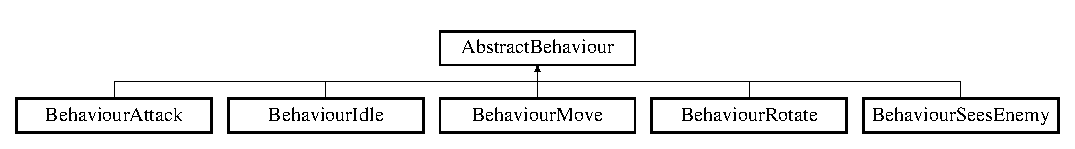
\includegraphics[height=1.555556cm]{class_abstract_behaviour}
\end{center}
\end{figure}
\subsection*{Public Member Functions}
\begin{DoxyCompactItemize}
\item 
\mbox{\Hypertarget{class_abstract_behaviour_a8a3a9217b3179f949a1d6a32f340c00c}\label{class_abstract_behaviour_a8a3a9217b3179f949a1d6a32f340c00c}} 
{\bfseries Abstract\+Behaviour} (shared\+\_\+ptr$<$ \mbox{\hyperlink{class_game_object}{Game\+Object}} $>$ self, shared\+\_\+ptr$<$ vector$<$ \mbox{\hyperlink{class_game_object}{Game\+Object}} $>$$>$ scene)
\item 
virtual void \mbox{\hyperlink{class_abstract_behaviour_ab99fb55a3b001e759e24d5b9721a742f}{execute}} ()=0
\begin{DoxyCompactList}\small\item\em Execute the behaviour. \end{DoxyCompactList}\end{DoxyCompactItemize}
\subsection*{Public Attributes}
\begin{DoxyCompactItemize}
\item 
\mbox{\Hypertarget{class_abstract_behaviour_a31b24fd948394c975ef56593e4ac0b28}\label{class_abstract_behaviour_a31b24fd948394c975ef56593e4ac0b28}} 
shared\+\_\+ptr$<$ \mbox{\hyperlink{class_abstract_behaviour}{Abstract\+Behaviour}} $>$ {\bfseries behaviour\+True} = nullptr
\item 
\mbox{\Hypertarget{class_abstract_behaviour_ad8e09f7cb5f6341b16f20845c8d3dd59}\label{class_abstract_behaviour_ad8e09f7cb5f6341b16f20845c8d3dd59}} 
shared\+\_\+ptr$<$ \mbox{\hyperlink{class_abstract_behaviour}{Abstract\+Behaviour}} $>$ {\bfseries behaviour\+False} = nullptr
\end{DoxyCompactItemize}
\subsection*{Protected Member Functions}
\begin{DoxyCompactItemize}
\item 
virtual void \mbox{\hyperlink{class_abstract_behaviour_a931021cf02c0a2dd40fac4a86d1d5d25}{execute\+Next\+Behaviour}} (bool is\+True)
\begin{DoxyCompactList}\small\item\em Execute the next behaviour. \end{DoxyCompactList}\end{DoxyCompactItemize}
\subsection*{Protected Attributes}
\begin{DoxyCompactItemize}
\item 
\mbox{\Hypertarget{class_abstract_behaviour_a4e825e734fdfe11ee2d030f909765845}\label{class_abstract_behaviour_a4e825e734fdfe11ee2d030f909765845}} 
shared\+\_\+ptr$<$ \mbox{\hyperlink{class_game_object}{Game\+Object}} $>$ {\bfseries \+\_\+self} = nullptr
\item 
\mbox{\Hypertarget{class_abstract_behaviour_a4c97685f487ce0f429276df8d003b70e}\label{class_abstract_behaviour_a4c97685f487ce0f429276df8d003b70e}} 
shared\+\_\+ptr$<$ vector$<$ \mbox{\hyperlink{class_game_object}{Game\+Object}} $>$ $>$ {\bfseries \+\_\+scene}
\end{DoxyCompactItemize}


\subsection{Detailed Description}
Abstract class for ai behavior 



\subsection{Member Function Documentation}
\mbox{\Hypertarget{class_abstract_behaviour_ab99fb55a3b001e759e24d5b9721a742f}\label{class_abstract_behaviour_ab99fb55a3b001e759e24d5b9721a742f}} 
\index{Abstract\+Behaviour@{Abstract\+Behaviour}!execute@{execute}}
\index{execute@{execute}!Abstract\+Behaviour@{Abstract\+Behaviour}}
\subsubsection{\texorpdfstring{execute()}{execute()}}
{\footnotesize\ttfamily virtual void Abstract\+Behaviour\+::execute (\begin{DoxyParamCaption}{ }\end{DoxyParamCaption})\hspace{0.3cm}{\ttfamily [pure virtual]}}



Execute the behaviour. 



Implemented in \mbox{\hyperlink{class_behaviour_attack_aca669f46a6d32e5e41e7b477be1ee4cf}{Behaviour\+Attack}}, \mbox{\hyperlink{class_behaviour_idle_ac810c315b1ea41772060b216ecdc2e11}{Behaviour\+Idle}}, \mbox{\hyperlink{class_behaviour_move_a4cccd6dbe5ccf37b1522fc71a807f080}{Behaviour\+Move}}, \mbox{\hyperlink{class_behaviour_rotate_aa01153f4a487813580ecb5d5145da47c}{Behaviour\+Rotate}}, and \mbox{\hyperlink{class_behaviour_sees_enemy_afddbf2ca7396c9fd7b24f4be60edb84c}{Behaviour\+Sees\+Enemy}}.

\mbox{\Hypertarget{class_abstract_behaviour_a931021cf02c0a2dd40fac4a86d1d5d25}\label{class_abstract_behaviour_a931021cf02c0a2dd40fac4a86d1d5d25}} 
\index{Abstract\+Behaviour@{Abstract\+Behaviour}!execute\+Next\+Behaviour@{execute\+Next\+Behaviour}}
\index{execute\+Next\+Behaviour@{execute\+Next\+Behaviour}!Abstract\+Behaviour@{Abstract\+Behaviour}}
\subsubsection{\texorpdfstring{execute\+Next\+Behaviour()}{executeNextBehaviour()}}
{\footnotesize\ttfamily void Abstract\+Behaviour\+::execute\+Next\+Behaviour (\begin{DoxyParamCaption}\item[{bool}]{is\+True }\end{DoxyParamCaption})\hspace{0.3cm}{\ttfamily [protected]}, {\ttfamily [virtual]}}



Execute the next behaviour. 


\begin{DoxyParams}{Parameters}
{\em is\+True} & The state of the next behaviour.\\
\hline
\end{DoxyParams}


The documentation for this class was generated from the following files\+:\begin{DoxyCompactItemize}
\item 
Abstract\+Behaviour.\+h\item 
Abstract\+Behaviour.\+cpp\end{DoxyCompactItemize}

\hypertarget{class_abstract_collision_resolution_extension}{}\section{Abstract\+Collision\+Resolution\+Extension Class Reference}
\label{class_abstract_collision_resolution_extension}\index{Abstract\+Collision\+Resolution\+Extension@{Abstract\+Collision\+Resolution\+Extension}}
Inheritance diagram for Abstract\+Collision\+Resolution\+Extension\+:\begin{figure}[H]
\begin{center}
\leavevmode
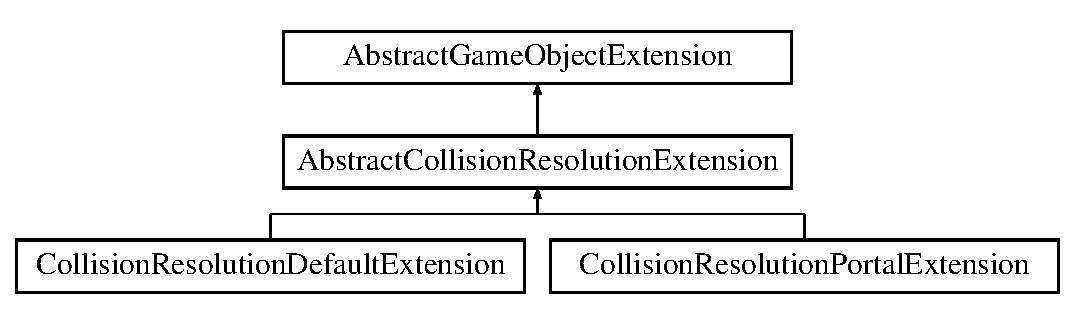
\includegraphics[height=3.000000cm]{class_abstract_collision_resolution_extension}
\end{center}
\end{figure}
\subsection*{Public Member Functions}
\begin{DoxyCompactItemize}
\item 
\mbox{\Hypertarget{class_abstract_collision_resolution_extension_a19e262b7077616a21245bd17e445bc86}\label{class_abstract_collision_resolution_extension_a19e262b7077616a21245bd17e445bc86}} 
virtual bool {\bfseries is\+Default} ()=0
\item 
\mbox{\Hypertarget{class_abstract_collision_resolution_extension_a4997ac66abd4356c47bdbca81c4324ce}\label{class_abstract_collision_resolution_extension_a4997ac66abd4356c47bdbca81c4324ce}} 
virtual void {\bfseries resolve\+Collision} (shared\+\_\+ptr$<$ \mbox{\hyperlink{class_game_object}{Game\+Object}} $>$ other\+Object)=0
\end{DoxyCompactItemize}
\subsection*{Additional Inherited Members}


The documentation for this class was generated from the following file\+:\begin{DoxyCompactItemize}
\item 
Abstract\+Collision\+Resolution\+Extension.\+h\end{DoxyCompactItemize}

\hypertarget{class_abstract_entity_a_i}{}\section{Abstract\+Entity\+AI Class Reference}
\label{class_abstract_entity_a_i}\index{Abstract\+Entity\+AI@{Abstract\+Entity\+AI}}


Abstract class for entity ai  




{\ttfamily \#include $<$Abstract\+Entity\+Ai.\+h$>$}

Inheritance diagram for Abstract\+Entity\+AI\+:\begin{figure}[H]
\begin{center}
\leavevmode
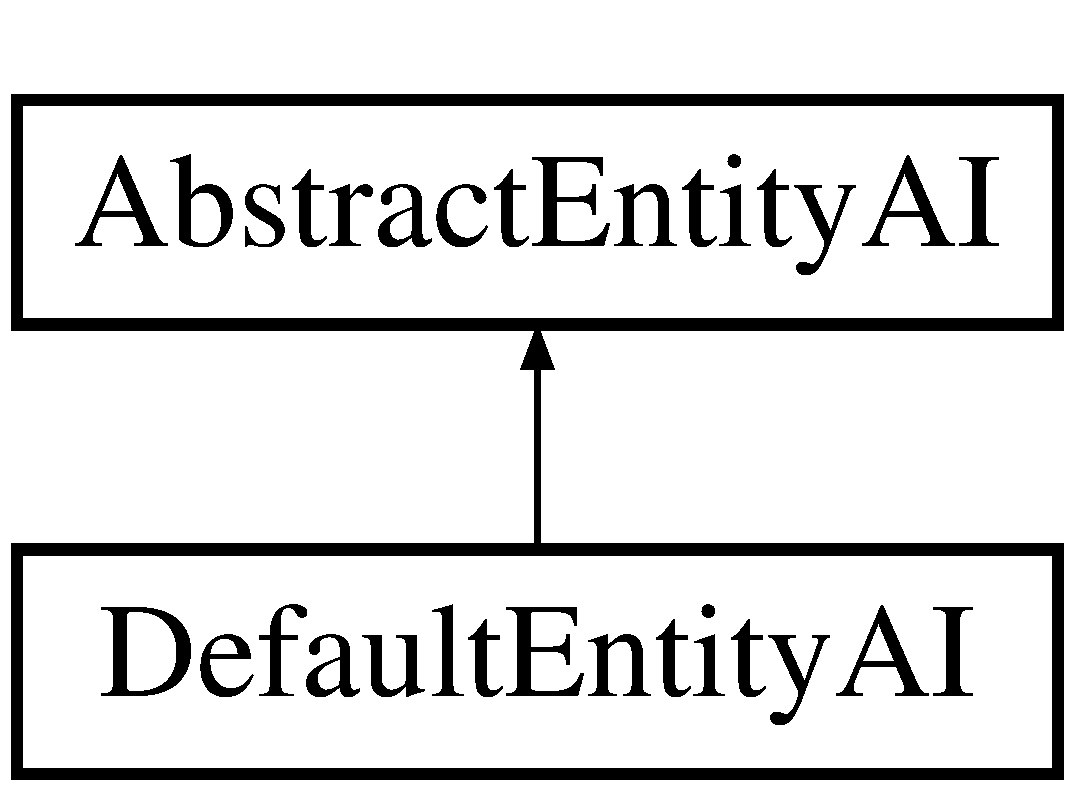
\includegraphics[height=2.000000cm]{class_abstract_entity_a_i}
\end{center}
\end{figure}
\subsection*{Public Member Functions}
\begin{DoxyCompactItemize}
\item 
\mbox{\Hypertarget{class_abstract_entity_a_i_a8dd5f0ed0b97b8089b1e0a7e67754bff}\label{class_abstract_entity_a_i_a8dd5f0ed0b97b8089b1e0a7e67754bff}} 
virtual void {\bfseries create\+Behaviour\+Tree} (shared\+\_\+ptr$<$ \mbox{\hyperlink{class_game_object}{Game\+Object}} $>$ self, shared\+\_\+ptr$<$ vector$<$ \mbox{\hyperlink{class_game_object}{Game\+Object}} $>$$>$ scene)=0
\end{DoxyCompactItemize}


\subsection{Detailed Description}
Abstract class for entity ai 



The documentation for this class was generated from the following files\+:\begin{DoxyCompactItemize}
\item 
Abstract\+Entity\+Ai.\+h\item 
Abstract\+Entity\+Ai.\+cpp\end{DoxyCompactItemize}

\hypertarget{class_abstract_game}{}\section{Abstract\+Game Class Reference}
\label{class_abstract_game}\index{Abstract\+Game@{Abstract\+Game}}


The game class needs to be based of this class.  




{\ttfamily \#include $<$Abstract\+Game.\+h$>$}

Inheritance diagram for Abstract\+Game\+:\begin{figure}[H]
\begin{center}
\leavevmode
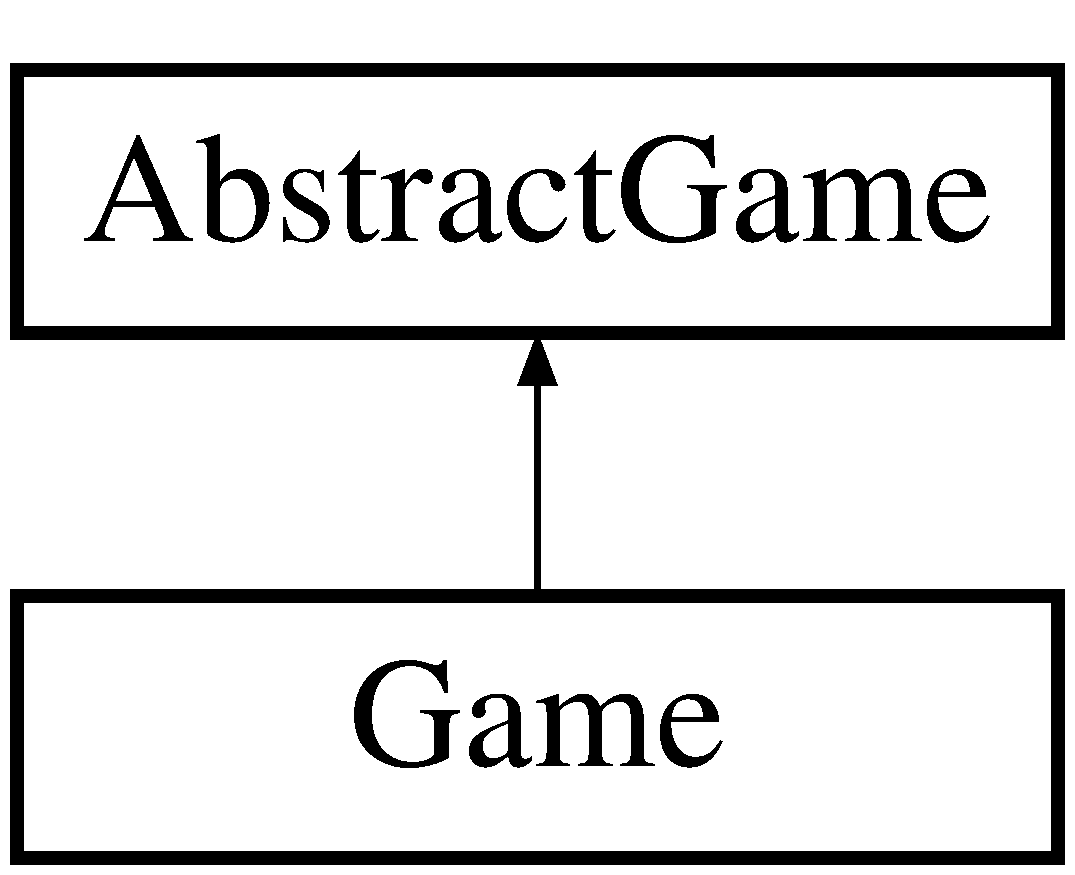
\includegraphics[height=2.000000cm]{class_abstract_game}
\end{center}
\end{figure}
\subsection*{Public Member Functions}
\begin{DoxyCompactItemize}
\item 
virtual void \mbox{\hyperlink{class_abstract_game_ae0bd76d926812f81e5e637ade3b1015f}{on\+Init}} ()=0
\begin{DoxyCompactList}\small\item\em Prepare the game. \end{DoxyCompactList}\item 
virtual void \mbox{\hyperlink{class_abstract_game_afd50e09c9b23aff40c752990947f07ce}{switch\+Screen}} (int screen\+Index)=0
\begin{DoxyCompactList}\small\item\em Switch the current screen to the screen with the given index \end{DoxyCompactList}\end{DoxyCompactItemize}
\subsection*{Public Attributes}
\begin{DoxyCompactItemize}
\item 
vector$<$ shared\+\_\+ptr$<$ \mbox{\hyperlink{class_abstract_screen}{Abstract\+Screen}} $>$ $>$ \mbox{\hyperlink{class_abstract_game_add5999d1c4190a9ad25dfdb51327720b}{screens}}
\begin{DoxyCompactList}\small\item\em All the possible screens the game has. \end{DoxyCompactList}\end{DoxyCompactItemize}
\subsection*{Protected Attributes}
\begin{DoxyCompactItemize}
\item 
int \mbox{\hyperlink{class_abstract_game_ab5e3089bdd788319c1a240992018c355}{\+\_\+active\+Screen}}
\begin{DoxyCompactList}\small\item\em The index of the visible screen. \end{DoxyCompactList}\item 
\mbox{\Hypertarget{class_abstract_game_ade8925d7eb607087ac30dbe0239b9a99}\label{class_abstract_game_ade8925d7eb607087ac30dbe0239b9a99}} 
\mbox{\hyperlink{struct_s_d_l_wrapper}{S\+D\+L\+Wrapper}} {\bfseries \+\_\+sdl}
\item 
\mbox{\Hypertarget{class_abstract_game_a9c7d0cf75caa0964f71df6fbb8f96fc6}\label{class_abstract_game_a9c7d0cf75caa0964f71df6fbb8f96fc6}} 
\mbox{\hyperlink{struct_s_d_l_image_wrapper}{S\+D\+L\+Image\+Wrapper}} {\bfseries \+\_\+sdl\+Image}
\item 
\mbox{\Hypertarget{class_abstract_game_adf290429d252d8209fcb4a6d8f879340}\label{class_abstract_game_adf290429d252d8209fcb4a6d8f879340}} 
\mbox{\hyperlink{struct_s_d_l_ttf_wrapper}{S\+D\+L\+Ttf\+Wrapper}} {\bfseries \+\_\+sdl\+Ttf}
\item 
\mbox{\Hypertarget{class_abstract_game_aae4bc7ee9bd867ea9f072113dabf3e6f}\label{class_abstract_game_aae4bc7ee9bd867ea9f072113dabf3e6f}} 
\mbox{\hyperlink{class_window}{Window}} $\ast$ {\bfseries \+\_\+window}
\end{DoxyCompactItemize}


\subsection{Detailed Description}
The game class needs to be based of this class. 



\subsection{Member Function Documentation}
\mbox{\Hypertarget{class_abstract_game_ae0bd76d926812f81e5e637ade3b1015f}\label{class_abstract_game_ae0bd76d926812f81e5e637ade3b1015f}} 
\index{Abstract\+Game@{Abstract\+Game}!on\+Init@{on\+Init}}
\index{on\+Init@{on\+Init}!Abstract\+Game@{Abstract\+Game}}
\subsubsection{\texorpdfstring{on\+Init()}{onInit()}}
{\footnotesize\ttfamily virtual void Abstract\+Game\+::on\+Init (\begin{DoxyParamCaption}{ }\end{DoxyParamCaption})\hspace{0.3cm}{\ttfamily [pure virtual]}}



Prepare the game. 



Implemented in \mbox{\hyperlink{class_game_a91946f348c9334abd083dfebfecdd31d}{Game}}.

\mbox{\Hypertarget{class_abstract_game_afd50e09c9b23aff40c752990947f07ce}\label{class_abstract_game_afd50e09c9b23aff40c752990947f07ce}} 
\index{Abstract\+Game@{Abstract\+Game}!switch\+Screen@{switch\+Screen}}
\index{switch\+Screen@{switch\+Screen}!Abstract\+Game@{Abstract\+Game}}
\subsubsection{\texorpdfstring{switch\+Screen()}{switchScreen()}}
{\footnotesize\ttfamily virtual void Abstract\+Game\+::switch\+Screen (\begin{DoxyParamCaption}\item[{int}]{screen\+Index }\end{DoxyParamCaption})\hspace{0.3cm}{\ttfamily [pure virtual]}}



Switch the current screen to the screen with the given index 


\begin{DoxyParams}{Parameters}
{\em screen\+Index} & The index of the screen we want to display\\
\hline
\end{DoxyParams}


Implemented in \mbox{\hyperlink{class_game_a0e1dd146112c54290e11d3e5f0a36fdd}{Game}}.



\subsection{Member Data Documentation}
\mbox{\Hypertarget{class_abstract_game_ab5e3089bdd788319c1a240992018c355}\label{class_abstract_game_ab5e3089bdd788319c1a240992018c355}} 
\index{Abstract\+Game@{Abstract\+Game}!\+\_\+active\+Screen@{\+\_\+active\+Screen}}
\index{\+\_\+active\+Screen@{\+\_\+active\+Screen}!Abstract\+Game@{Abstract\+Game}}
\subsubsection{\texorpdfstring{\+\_\+active\+Screen}{\_activeScreen}}
{\footnotesize\ttfamily int Abstract\+Game\+::\+\_\+active\+Screen\hspace{0.3cm}{\ttfamily [protected]}}



The index of the visible screen. 

\mbox{\Hypertarget{class_abstract_game_add5999d1c4190a9ad25dfdb51327720b}\label{class_abstract_game_add5999d1c4190a9ad25dfdb51327720b}} 
\index{Abstract\+Game@{Abstract\+Game}!screens@{screens}}
\index{screens@{screens}!Abstract\+Game@{Abstract\+Game}}
\subsubsection{\texorpdfstring{screens}{screens}}
{\footnotesize\ttfamily vector$<$shared\+\_\+ptr$<$\mbox{\hyperlink{class_abstract_screen}{Abstract\+Screen}}$>$ $>$ Abstract\+Game\+::screens}



All the possible screens the game has. 



The documentation for this class was generated from the following files\+:\begin{DoxyCompactItemize}
\item 
Abstract\+Game.\+h\item 
Abstract\+Game.\+cpp\end{DoxyCompactItemize}

\hypertarget{class_abstract_game_object_extension}{}\section{Abstract\+Game\+Object\+Extension Class Reference}
\label{class_abstract_game_object_extension}\index{Abstract\+Game\+Object\+Extension@{Abstract\+Game\+Object\+Extension}}
Inheritance diagram for Abstract\+Game\+Object\+Extension\+:\begin{figure}[H]
\begin{center}
\leavevmode
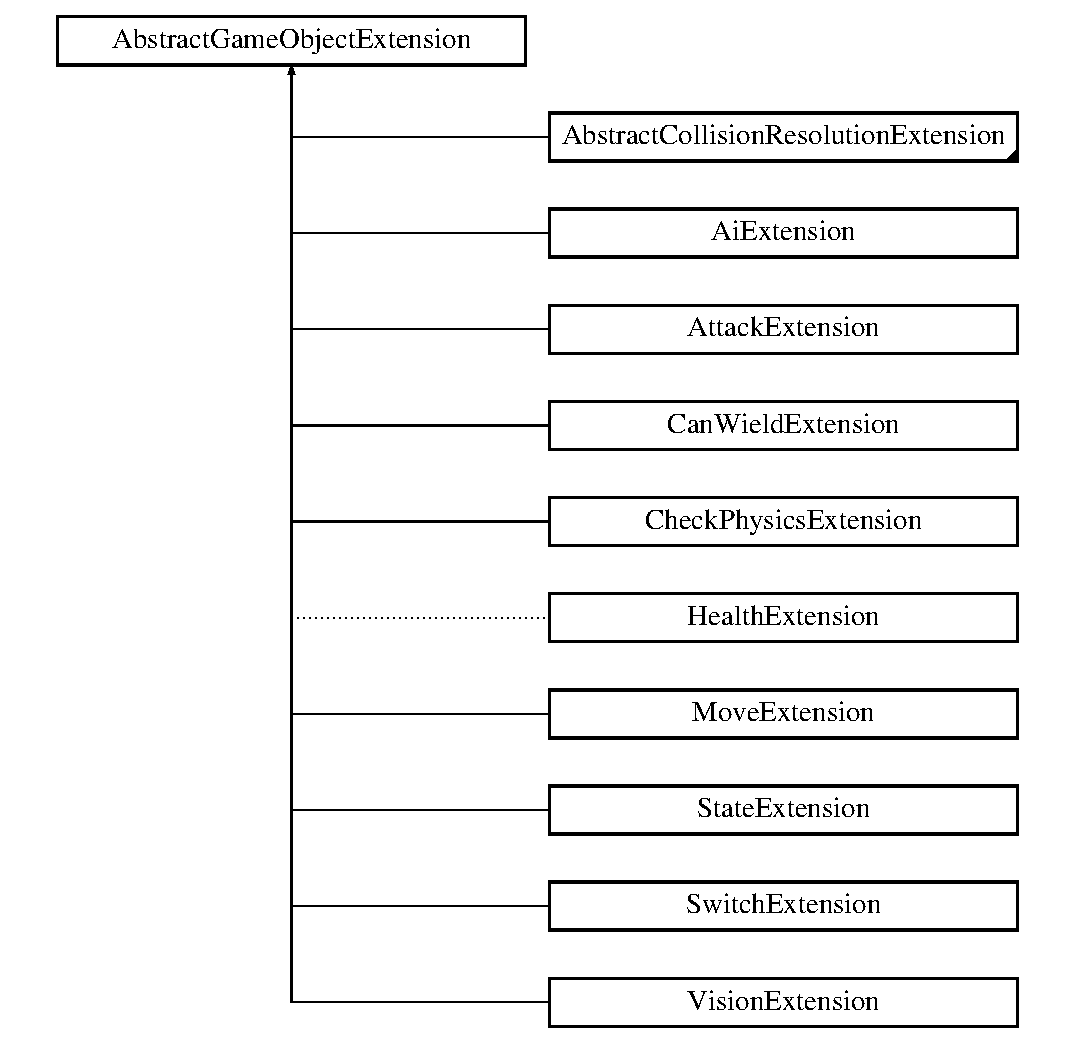
\includegraphics[height=11.000000cm]{class_abstract_game_object_extension}
\end{center}
\end{figure}
\subsection*{Public Member Functions}
\begin{DoxyCompactItemize}
\item 
\mbox{\Hypertarget{class_abstract_game_object_extension_abaa841674842d2e85cb65413bbbf4fb1}\label{class_abstract_game_object_extension_abaa841674842d2e85cb65413bbbf4fb1}} 
virtual void {\bfseries register\+Subject} (shared\+\_\+ptr$<$ \mbox{\hyperlink{class_game_object}{Game\+Object}} $>$ subject)
\end{DoxyCompactItemize}
\subsection*{Public Attributes}
\begin{DoxyCompactItemize}
\item 
\mbox{\Hypertarget{class_abstract_game_object_extension_a75e13466dc5bb8809dc1c843776364df}\label{class_abstract_game_object_extension_a75e13466dc5bb8809dc1c843776364df}} 
string {\bfseries type}
\end{DoxyCompactItemize}
\subsection*{Protected Attributes}
\begin{DoxyCompactItemize}
\item 
\mbox{\Hypertarget{class_abstract_game_object_extension_a4fb454cd6286777bdf6804239dc93e51}\label{class_abstract_game_object_extension_a4fb454cd6286777bdf6804239dc93e51}} 
shared\+\_\+ptr$<$ \mbox{\hyperlink{class_game_object}{Game\+Object}} $>$ {\bfseries \+\_\+subject}
\end{DoxyCompactItemize}


The documentation for this class was generated from the following files\+:\begin{DoxyCompactItemize}
\item 
Abstract\+Game\+Object\+Extension.\+h\item 
Abstract\+Game\+Object\+Extension.\+cpp\end{DoxyCompactItemize}

\hypertarget{class_abstract_manageable_item}{}\section{Abstract\+Manageable\+Item Class Reference}
\label{class_abstract_manageable_item}\index{Abstract\+Manageable\+Item@{Abstract\+Manageable\+Item}}


The documentation for this class was generated from the following file\+:\begin{DoxyCompactItemize}
\item 
Abstract\+Manageable\+Item.\+h\end{DoxyCompactItemize}

\hypertarget{class_abstract_screen}{}\section{Abstract\+Screen Class Reference}
\label{class_abstract_screen}\index{Abstract\+Screen@{Abstract\+Screen}}
Inheritance diagram for Abstract\+Screen\+:\begin{figure}[H]
\begin{center}
\leavevmode
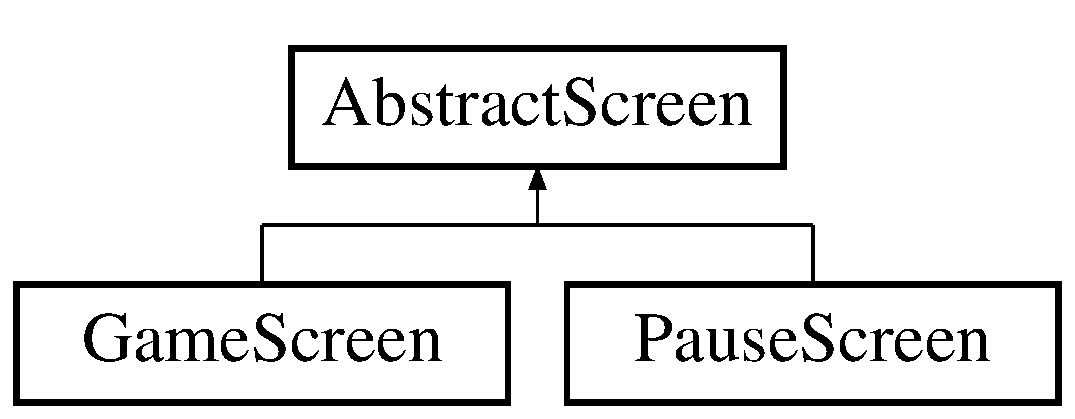
\includegraphics[height=1.851240cm]{class_abstract_screen}
\end{center}
\end{figure}
\subsection*{Public Types}
\begin{DoxyCompactItemize}
\item 
enum \mbox{\hyperlink{class_abstract_screen_a837c6697225dad22e41a384fde73c16b}{Screens}} \{ \newline
{\bfseries Main\+Game} = 0, 
{\bfseries Pause}, 
{\bfseries Credits}, 
{\bfseries Help}, 
\newline
{\bfseries Main\+Menu}
 \}
\begin{DoxyCompactList}\small\item\em Screen enums has to be in right order the order the screens get created \end{DoxyCompactList}\end{DoxyCompactItemize}
\subsection*{Public Member Functions}
\begin{DoxyCompactItemize}
\item 
virtual void \mbox{\hyperlink{class_abstract_screen_a7ab389bd33f4824d3d353b5a9e1616de}{on\+Init}} ()=0
\begin{DoxyCompactList}\small\item\em Called one time to create all objects. \end{DoxyCompactList}\item 
virtual void \mbox{\hyperlink{class_abstract_screen_a3861213630fd23d4a3ff392191614ec2}{on\+Tick}} ()=0
\begin{DoxyCompactList}\small\item\em Called every tick to update properties. \end{DoxyCompactList}\item 
virtual void \mbox{\hyperlink{class_abstract_screen_a219687a34e6aed15a9eaf0d4414d1783}{on\+Screen\+Showed}} ()=0
\begin{DoxyCompactList}\small\item\em Called when the user switches to this screen. \end{DoxyCompactList}\item 
virtual void \mbox{\hyperlink{class_abstract_screen_ad618b78e55faf59bab580e920461b790}{handle\+Keyboard\+Input}} (S\+D\+L\+\_\+\+Keyboard\+Event e)=0
\begin{DoxyCompactList}\small\item\em Called when the user uses their keyboard. \end{DoxyCompactList}\item 
virtual void \mbox{\hyperlink{class_abstract_screen_ab05039a94ee494811800187787636d2b}{handle\+Mouse\+Motion\+Input}} (S\+D\+L\+\_\+\+Mouse\+Motion\+Event e)=0
\begin{DoxyCompactList}\small\item\em Called when the user moves their mouse. \end{DoxyCompactList}\item 
virtual void \mbox{\hyperlink{class_abstract_screen_a9f9631ff1a9078b96bcf31e062f7379e}{handle\+Mouse\+Click\+Input}} (S\+D\+L\+\_\+\+Mouse\+Button\+Event e)=0
\begin{DoxyCompactList}\small\item\em Called when the user click their mouse. \end{DoxyCompactList}\item 
virtual void \mbox{\hyperlink{class_abstract_screen_a64d29254d2ad4f9c8050e8f56d3c27a8}{register\+Game}} (\mbox{\hyperlink{class_abstract_game}{Abstract\+Game}} $\ast$game)
\begin{DoxyCompactList}\small\item\em Adds a reference to the game. \end{DoxyCompactList}\end{DoxyCompactItemize}
\subsection*{Public Attributes}
\begin{DoxyCompactItemize}
\item 
\mbox{\Hypertarget{class_abstract_screen_a4898cec711e7cdc71bcc46399e4e1a4e}\label{class_abstract_screen_a4898cec711e7cdc71bcc46399e4e1a4e}} 
vector$<$ shared\+\_\+ptr$<$ \mbox{\hyperlink{class_game_object}{Game\+Object}} $>$ $>$ {\bfseries game\+Objects}
\item 
\mbox{\Hypertarget{class_abstract_screen_a09109f46ca7d8662cf0b2d6c49931196}\label{class_abstract_screen_a09109f46ca7d8662cf0b2d6c49931196}} 
vector$<$ shared\+\_\+ptr$<$ \mbox{\hyperlink{class_abstract_ui_element}{Abstract\+Ui\+Element}} $>$ $>$ {\bfseries ui\+Elements}
\end{DoxyCompactItemize}
\subsection*{Protected Attributes}
\begin{DoxyCompactItemize}
\item 
\mbox{\Hypertarget{class_abstract_screen_ade20515e2fc913122f74f1989b41c15c}\label{class_abstract_screen_ade20515e2fc913122f74f1989b41c15c}} 
\mbox{\hyperlink{class_abstract_game}{Abstract\+Game}} $\ast$ {\bfseries \+\_\+game}
\end{DoxyCompactItemize}


\subsection{Member Enumeration Documentation}
\mbox{\Hypertarget{class_abstract_screen_a837c6697225dad22e41a384fde73c16b}\label{class_abstract_screen_a837c6697225dad22e41a384fde73c16b}} 
\index{Abstract\+Screen@{Abstract\+Screen}!Screens@{Screens}}
\index{Screens@{Screens}!Abstract\+Screen@{Abstract\+Screen}}
\subsubsection{\texorpdfstring{Screens}{Screens}}
{\footnotesize\ttfamily enum \mbox{\hyperlink{class_abstract_screen_a837c6697225dad22e41a384fde73c16b}{Abstract\+Screen\+::\+Screens}}}



Screen enums has to be in right order the order the screens get created 



\subsection{Member Function Documentation}
\mbox{\Hypertarget{class_abstract_screen_ad618b78e55faf59bab580e920461b790}\label{class_abstract_screen_ad618b78e55faf59bab580e920461b790}} 
\index{Abstract\+Screen@{Abstract\+Screen}!handle\+Keyboard\+Input@{handle\+Keyboard\+Input}}
\index{handle\+Keyboard\+Input@{handle\+Keyboard\+Input}!Abstract\+Screen@{Abstract\+Screen}}
\subsubsection{\texorpdfstring{handle\+Keyboard\+Input()}{handleKeyboardInput()}}
{\footnotesize\ttfamily virtual void Abstract\+Screen\+::handle\+Keyboard\+Input (\begin{DoxyParamCaption}\item[{S\+D\+L\+\_\+\+Keyboard\+Event}]{e }\end{DoxyParamCaption})\hspace{0.3cm}{\ttfamily [pure virtual]}}



Called when the user uses their keyboard. 


\begin{DoxyParams}{Parameters}
{\em e} & The keyboard event.\\
\hline
\end{DoxyParams}


Implemented in \mbox{\hyperlink{class_game_screen_ae0cb9f2e2ca4016debdffa7f778f5627}{Game\+Screen}}, \mbox{\hyperlink{class_main_menu_screen_a05a9d0a6723772ceaa6ab78f80bbee79}{Main\+Menu\+Screen}}, \mbox{\hyperlink{class_pause_screen_a94112a789c88bdf68809b09ec86049c8}{Pause\+Screen}}, \mbox{\hyperlink{class_credits_screen_ad0bbbfee8f8c6147c300228332e4779a}{Credits\+Screen}}, and \mbox{\hyperlink{class_help_screen_ad64812fb3118933e661b5bcf792f52ce}{Help\+Screen}}.

\mbox{\Hypertarget{class_abstract_screen_a9f9631ff1a9078b96bcf31e062f7379e}\label{class_abstract_screen_a9f9631ff1a9078b96bcf31e062f7379e}} 
\index{Abstract\+Screen@{Abstract\+Screen}!handle\+Mouse\+Click\+Input@{handle\+Mouse\+Click\+Input}}
\index{handle\+Mouse\+Click\+Input@{handle\+Mouse\+Click\+Input}!Abstract\+Screen@{Abstract\+Screen}}
\subsubsection{\texorpdfstring{handle\+Mouse\+Click\+Input()}{handleMouseClickInput()}}
{\footnotesize\ttfamily virtual void Abstract\+Screen\+::handle\+Mouse\+Click\+Input (\begin{DoxyParamCaption}\item[{S\+D\+L\+\_\+\+Mouse\+Button\+Event}]{e }\end{DoxyParamCaption})\hspace{0.3cm}{\ttfamily [pure virtual]}}



Called when the user click their mouse. 


\begin{DoxyParams}{Parameters}
{\em e} & The mouse click event.\\
\hline
\end{DoxyParams}


Implemented in \mbox{\hyperlink{class_game_screen_abe56a9ed6eaac0df7459f681265e0dd2}{Game\+Screen}}, \mbox{\hyperlink{class_main_menu_screen_acd91967ce0abc90ef3d4c70099a8a4f8}{Main\+Menu\+Screen}}, \mbox{\hyperlink{class_pause_screen_a82ce01aa34df937a0f072d6210ac4386}{Pause\+Screen}}, \mbox{\hyperlink{class_credits_screen_a5f913193cac127f2f73156b6885931d2}{Credits\+Screen}}, and \mbox{\hyperlink{class_help_screen_ac4c015df8c6ea1e8963412ce1095c369}{Help\+Screen}}.

\mbox{\Hypertarget{class_abstract_screen_ab05039a94ee494811800187787636d2b}\label{class_abstract_screen_ab05039a94ee494811800187787636d2b}} 
\index{Abstract\+Screen@{Abstract\+Screen}!handle\+Mouse\+Motion\+Input@{handle\+Mouse\+Motion\+Input}}
\index{handle\+Mouse\+Motion\+Input@{handle\+Mouse\+Motion\+Input}!Abstract\+Screen@{Abstract\+Screen}}
\subsubsection{\texorpdfstring{handle\+Mouse\+Motion\+Input()}{handleMouseMotionInput()}}
{\footnotesize\ttfamily virtual void Abstract\+Screen\+::handle\+Mouse\+Motion\+Input (\begin{DoxyParamCaption}\item[{S\+D\+L\+\_\+\+Mouse\+Motion\+Event}]{e }\end{DoxyParamCaption})\hspace{0.3cm}{\ttfamily [pure virtual]}}



Called when the user moves their mouse. 


\begin{DoxyParams}{Parameters}
{\em e} & The mouse mouse event.\\
\hline
\end{DoxyParams}


Implemented in \mbox{\hyperlink{class_game_screen_af2fbc9a94d5b522870a9bfceea0f1da5}{Game\+Screen}}, \mbox{\hyperlink{class_main_menu_screen_a5f00aa37c3ebe01824e3d23af9b55bae}{Main\+Menu\+Screen}}, \mbox{\hyperlink{class_pause_screen_a19ce9a528ab648afb81a2251810afcfa}{Pause\+Screen}}, \mbox{\hyperlink{class_credits_screen_ad20f8d95b70339755f42736a0f1e6e38}{Credits\+Screen}}, and \mbox{\hyperlink{class_help_screen_a0e93b5a0c01835842e5e7082762a0dbf}{Help\+Screen}}.

\mbox{\Hypertarget{class_abstract_screen_a7ab389bd33f4824d3d353b5a9e1616de}\label{class_abstract_screen_a7ab389bd33f4824d3d353b5a9e1616de}} 
\index{Abstract\+Screen@{Abstract\+Screen}!on\+Init@{on\+Init}}
\index{on\+Init@{on\+Init}!Abstract\+Screen@{Abstract\+Screen}}
\subsubsection{\texorpdfstring{on\+Init()}{onInit()}}
{\footnotesize\ttfamily virtual void Abstract\+Screen\+::on\+Init (\begin{DoxyParamCaption}{ }\end{DoxyParamCaption})\hspace{0.3cm}{\ttfamily [pure virtual]}}



Called one time to create all objects. 



Implemented in \mbox{\hyperlink{class_game_screen_a2748a44cf5e9ebe46f4e2e603bbfbae3}{Game\+Screen}}, \mbox{\hyperlink{class_main_menu_screen_a700bf80fbcb9d6f4110347f73b8c6e09}{Main\+Menu\+Screen}}, \mbox{\hyperlink{class_pause_screen_ae8196adf49b2e7439677a5360a8d43d4}{Pause\+Screen}}, \mbox{\hyperlink{class_credits_screen_a614ba7f8090fb0a69a31062a31bcbb86}{Credits\+Screen}}, and \mbox{\hyperlink{class_help_screen_a2649a31d286a6721dde6f87c2536d5c5}{Help\+Screen}}.

\mbox{\Hypertarget{class_abstract_screen_a219687a34e6aed15a9eaf0d4414d1783}\label{class_abstract_screen_a219687a34e6aed15a9eaf0d4414d1783}} 
\index{Abstract\+Screen@{Abstract\+Screen}!on\+Screen\+Showed@{on\+Screen\+Showed}}
\index{on\+Screen\+Showed@{on\+Screen\+Showed}!Abstract\+Screen@{Abstract\+Screen}}
\subsubsection{\texorpdfstring{on\+Screen\+Showed()}{onScreenShowed()}}
{\footnotesize\ttfamily virtual void Abstract\+Screen\+::on\+Screen\+Showed (\begin{DoxyParamCaption}{ }\end{DoxyParamCaption})\hspace{0.3cm}{\ttfamily [pure virtual]}}



Called when the user switches to this screen. 



Implemented in \mbox{\hyperlink{class_game_screen_a1dfaea8cc8d0edb3bd2711d20e97ebeb}{Game\+Screen}}, \mbox{\hyperlink{class_main_menu_screen_a484fb745ff8ad64b2533ff31f38c7a0c}{Main\+Menu\+Screen}}, \mbox{\hyperlink{class_pause_screen_a2eb2b032a3c3e833beb505c2df12396b}{Pause\+Screen}}, \mbox{\hyperlink{class_credits_screen_a3fd4bc101df8b7560ab590c07997d472}{Credits\+Screen}}, and \mbox{\hyperlink{class_help_screen_a65d1845f657954d98e60cd042020c518}{Help\+Screen}}.

\mbox{\Hypertarget{class_abstract_screen_a3861213630fd23d4a3ff392191614ec2}\label{class_abstract_screen_a3861213630fd23d4a3ff392191614ec2}} 
\index{Abstract\+Screen@{Abstract\+Screen}!on\+Tick@{on\+Tick}}
\index{on\+Tick@{on\+Tick}!Abstract\+Screen@{Abstract\+Screen}}
\subsubsection{\texorpdfstring{on\+Tick()}{onTick()}}
{\footnotesize\ttfamily virtual void Abstract\+Screen\+::on\+Tick (\begin{DoxyParamCaption}{ }\end{DoxyParamCaption})\hspace{0.3cm}{\ttfamily [pure virtual]}}



Called every tick to update properties. 



Implemented in \mbox{\hyperlink{class_game_screen_a0e2549c9c0198f925df16203998bb53b}{Game\+Screen}}, \mbox{\hyperlink{class_main_menu_screen_aed1487c5d901c0a94ff960681f141024}{Main\+Menu\+Screen}}, \mbox{\hyperlink{class_pause_screen_a89ef5189bdc9acfae5eedbff2cf4b458}{Pause\+Screen}}, \mbox{\hyperlink{class_credits_screen_aa6eab21c9a72bda052da4a68e384df62}{Credits\+Screen}}, and \mbox{\hyperlink{class_help_screen_acb766ebc2fcf05e146bf808618fa57c6}{Help\+Screen}}.

\mbox{\Hypertarget{class_abstract_screen_a64d29254d2ad4f9c8050e8f56d3c27a8}\label{class_abstract_screen_a64d29254d2ad4f9c8050e8f56d3c27a8}} 
\index{Abstract\+Screen@{Abstract\+Screen}!register\+Game@{register\+Game}}
\index{register\+Game@{register\+Game}!Abstract\+Screen@{Abstract\+Screen}}
\subsubsection{\texorpdfstring{register\+Game()}{registerGame()}}
{\footnotesize\ttfamily void Abstract\+Screen\+::register\+Game (\begin{DoxyParamCaption}\item[{\mbox{\hyperlink{class_abstract_game}{Abstract\+Game}} $\ast$}]{game }\end{DoxyParamCaption})\hspace{0.3cm}{\ttfamily [virtual]}}



Adds a reference to the game. 


\begin{DoxyParams}{Parameters}
{\em game} & A refrence to the game.\\
\hline
\end{DoxyParams}


The documentation for this class was generated from the following files\+:\begin{DoxyCompactItemize}
\item 
Abstract\+Screen.\+h\item 
Abstract\+Screen.\+cpp\end{DoxyCompactItemize}

\hypertarget{class_abstract_ui_element}{}\section{Abstract\+Ui\+Element Class Reference}
\label{class_abstract_ui_element}\index{Abstract\+Ui\+Element@{Abstract\+Ui\+Element}}
Inheritance diagram for Abstract\+Ui\+Element\+:\begin{figure}[H]
\begin{center}
\leavevmode
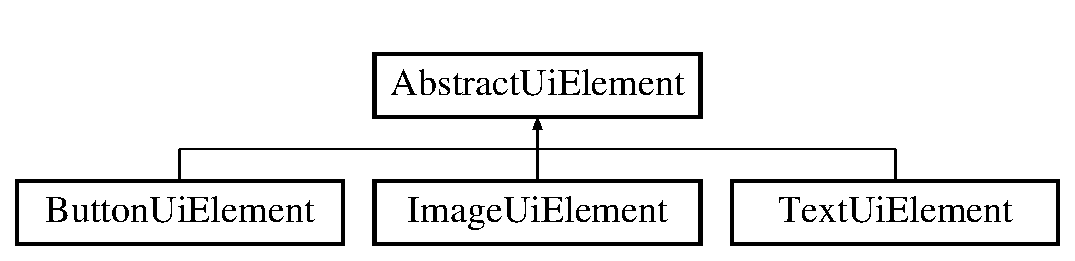
\includegraphics[height=2.000000cm]{class_abstract_ui_element}
\end{center}
\end{figure}
\subsection*{Public Member Functions}
\begin{DoxyCompactItemize}
\item 
virtual void \mbox{\hyperlink{class_abstract_ui_element_afacedc89a5805d95d3bdcf20619b1c06}{render}} (S\+D\+L\+\_\+\+Renderer $\ast$renderer)=0
\begin{DoxyCompactList}\small\item\em Render the element on the screen. \end{DoxyCompactList}\item 
virtual void \mbox{\hyperlink{class_abstract_ui_element_a42296c15c9e70b6ac7fda0b1862612af}{on\+Click}} ()=0
\begin{DoxyCompactList}\small\item\em The function executed when the element is clicked on. \end{DoxyCompactList}\item 
virtual bool \mbox{\hyperlink{class_abstract_ui_element_ad2c415461cd7e8c1ee50b1105eb84685}{is\+In\+Bound}} (int mouseX, int mouseY)=0
\begin{DoxyCompactList}\small\item\em Checks if the mouse is within the bounds of the element. \end{DoxyCompactList}\item 
virtual void \mbox{\hyperlink{class_abstract_ui_element_aea8a32a77e77f601ca114b8738072079}{register\+Game}} (\mbox{\hyperlink{class_abstract_game}{Abstract\+Game}} $\ast$game)
\begin{DoxyCompactList}\small\item\em Register the game to the element. \end{DoxyCompactList}\end{DoxyCompactItemize}
\subsection*{Protected Attributes}
\begin{DoxyCompactItemize}
\item 
\mbox{\Hypertarget{class_abstract_ui_element_ad80a25aa84eb844afd1c5e091063e8fb}\label{class_abstract_ui_element_ad80a25aa84eb844afd1c5e091063e8fb}} 
\mbox{\hyperlink{class_abstract_game}{Abstract\+Game}} $\ast$ {\bfseries \+\_\+game}
\item 
\mbox{\Hypertarget{class_abstract_ui_element_a91aa849cd7db2aac4b7dd36d6094961d}\label{class_abstract_ui_element_a91aa849cd7db2aac4b7dd36d6094961d}} 
S\+D\+L\+\_\+\+Rect {\bfseries \+\_\+rectangle}
\end{DoxyCompactItemize}


\subsection{Member Function Documentation}
\mbox{\Hypertarget{class_abstract_ui_element_ad2c415461cd7e8c1ee50b1105eb84685}\label{class_abstract_ui_element_ad2c415461cd7e8c1ee50b1105eb84685}} 
\index{Abstract\+Ui\+Element@{Abstract\+Ui\+Element}!is\+In\+Bound@{is\+In\+Bound}}
\index{is\+In\+Bound@{is\+In\+Bound}!Abstract\+Ui\+Element@{Abstract\+Ui\+Element}}
\subsubsection{\texorpdfstring{is\+In\+Bound()}{isInBound()}}
{\footnotesize\ttfamily virtual bool Abstract\+Ui\+Element\+::is\+In\+Bound (\begin{DoxyParamCaption}\item[{int}]{mouseX,  }\item[{int}]{mouseY }\end{DoxyParamCaption})\hspace{0.3cm}{\ttfamily [pure virtual]}}



Checks if the mouse is within the bounds of the element. 


\begin{DoxyParams}{Parameters}
{\em mouseX} & X coordinate of the mouse\\
\hline
{\em mouseY} & Y coordinate of the mouse\\
\hline
\end{DoxyParams}
\begin{DoxyReturn}{Returns}

\end{DoxyReturn}


Implemented in \mbox{\hyperlink{class_button_ui_element_ab321d646770df66f7ea58a7246d7bf28}{Button\+Ui\+Element}}, \mbox{\hyperlink{class_image_ui_element_a6d0f66cf68c5f035f5a9bfeaba3028f4}{Image\+Ui\+Element}}, and \mbox{\hyperlink{class_text_ui_element_aaf04a9d0a67e77e2ba2a306e1ec7aeed}{Text\+Ui\+Element}}.

\mbox{\Hypertarget{class_abstract_ui_element_a42296c15c9e70b6ac7fda0b1862612af}\label{class_abstract_ui_element_a42296c15c9e70b6ac7fda0b1862612af}} 
\index{Abstract\+Ui\+Element@{Abstract\+Ui\+Element}!on\+Click@{on\+Click}}
\index{on\+Click@{on\+Click}!Abstract\+Ui\+Element@{Abstract\+Ui\+Element}}
\subsubsection{\texorpdfstring{on\+Click()}{onClick()}}
{\footnotesize\ttfamily virtual void Abstract\+Ui\+Element\+::on\+Click (\begin{DoxyParamCaption}{ }\end{DoxyParamCaption})\hspace{0.3cm}{\ttfamily [pure virtual]}}



The function executed when the element is clicked on. 



Implemented in \mbox{\hyperlink{class_button_ui_element_a06c748ef9e81216f76d7db936d320365}{Button\+Ui\+Element}}, \mbox{\hyperlink{class_image_ui_element_ab3c388de0807d86016a2ff43fd6d337e}{Image\+Ui\+Element}}, and \mbox{\hyperlink{class_text_ui_element_a984d8bcd627f43c1bd858a707df2c042}{Text\+Ui\+Element}}.

\mbox{\Hypertarget{class_abstract_ui_element_aea8a32a77e77f601ca114b8738072079}\label{class_abstract_ui_element_aea8a32a77e77f601ca114b8738072079}} 
\index{Abstract\+Ui\+Element@{Abstract\+Ui\+Element}!register\+Game@{register\+Game}}
\index{register\+Game@{register\+Game}!Abstract\+Ui\+Element@{Abstract\+Ui\+Element}}
\subsubsection{\texorpdfstring{register\+Game()}{registerGame()}}
{\footnotesize\ttfamily void Abstract\+Ui\+Element\+::register\+Game (\begin{DoxyParamCaption}\item[{\mbox{\hyperlink{class_abstract_game}{Abstract\+Game}} $\ast$}]{game }\end{DoxyParamCaption})\hspace{0.3cm}{\ttfamily [virtual]}}



Register the game to the element. 


\begin{DoxyParams}{Parameters}
{\em game} & The \mbox{\hyperlink{class_game}{Game}}\\
\hline
\end{DoxyParams}
\mbox{\Hypertarget{class_abstract_ui_element_afacedc89a5805d95d3bdcf20619b1c06}\label{class_abstract_ui_element_afacedc89a5805d95d3bdcf20619b1c06}} 
\index{Abstract\+Ui\+Element@{Abstract\+Ui\+Element}!render@{render}}
\index{render@{render}!Abstract\+Ui\+Element@{Abstract\+Ui\+Element}}
\subsubsection{\texorpdfstring{render()}{render()}}
{\footnotesize\ttfamily virtual void Abstract\+Ui\+Element\+::render (\begin{DoxyParamCaption}\item[{S\+D\+L\+\_\+\+Renderer $\ast$}]{renderer }\end{DoxyParamCaption})\hspace{0.3cm}{\ttfamily [pure virtual]}}



Render the element on the screen. 


\begin{DoxyParams}{Parameters}
{\em renderer} & The renderer\\
\hline
\end{DoxyParams}


Implemented in \mbox{\hyperlink{class_button_ui_element_ad319e20e8abedefe07aef58a38ae9a81}{Button\+Ui\+Element}}, \mbox{\hyperlink{class_image_ui_element_a422fc1d3b4c1451f656e7470e575577b}{Image\+Ui\+Element}}, and \mbox{\hyperlink{class_text_ui_element_a7931ba283acdf102442a9181b3ddf276}{Text\+Ui\+Element}}.



The documentation for this class was generated from the following files\+:\begin{DoxyCompactItemize}
\item 
Abstract\+Ui\+Element.\+h\item 
Abstract\+Ui\+Element.\+cpp\end{DoxyCompactItemize}

\hypertarget{class_ai_extension}{}\section{Ai\+Extension Class Reference}
\label{class_ai_extension}\index{Ai\+Extension@{Ai\+Extension}}


AI Capabilities  




{\ttfamily \#include $<$Ai\+Extension.\+h$>$}

Inheritance diagram for Ai\+Extension\+:\begin{figure}[H]
\begin{center}
\leavevmode
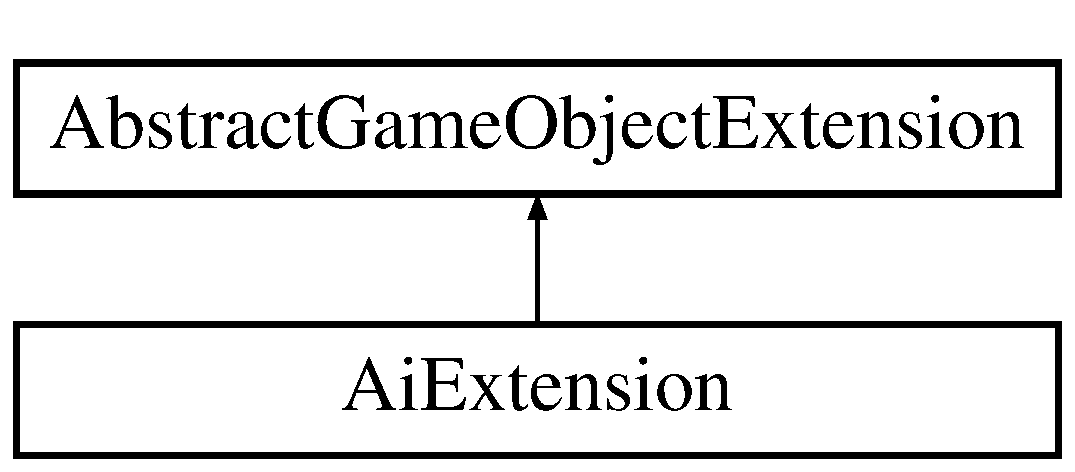
\includegraphics[height=2.000000cm]{class_ai_extension}
\end{center}
\end{figure}
\subsection*{Public Member Functions}
\begin{DoxyCompactItemize}
\item 
\mbox{\Hypertarget{class_ai_extension_ae409686820de2db2fc0125987500bc71}\label{class_ai_extension_ae409686820de2db2fc0125987500bc71}} 
void {\bfseries do\+Ai} ()
\end{DoxyCompactItemize}
\subsection*{Static Public Member Functions}
\begin{DoxyCompactItemize}
\item 
\mbox{\Hypertarget{class_ai_extension_ac6134bbf56c9f7bfd1e5707ca05475bf}\label{class_ai_extension_ac6134bbf56c9f7bfd1e5707ca05475bf}} 
static \mbox{\hyperlink{class_abstract_game_object_extension}{Abstract\+Game\+Object\+Extension}} $\ast$\+\_\+\+\_\+stdcall {\bfseries create} ()
\end{DoxyCompactItemize}
\subsection*{Additional Inherited Members}


\subsection{Detailed Description}
AI Capabilities 



The documentation for this class was generated from the following files\+:\begin{DoxyCompactItemize}
\item 
Ai\+Extension.\+h\item 
Ai\+Extension.\+cpp\end{DoxyCompactItemize}

\hypertarget{class_attack_extension}{}\section{Attack\+Extension Class Reference}
\label{class_attack_extension}\index{Attack\+Extension@{Attack\+Extension}}
Inheritance diagram for Attack\+Extension\+:\begin{figure}[H]
\begin{center}
\leavevmode
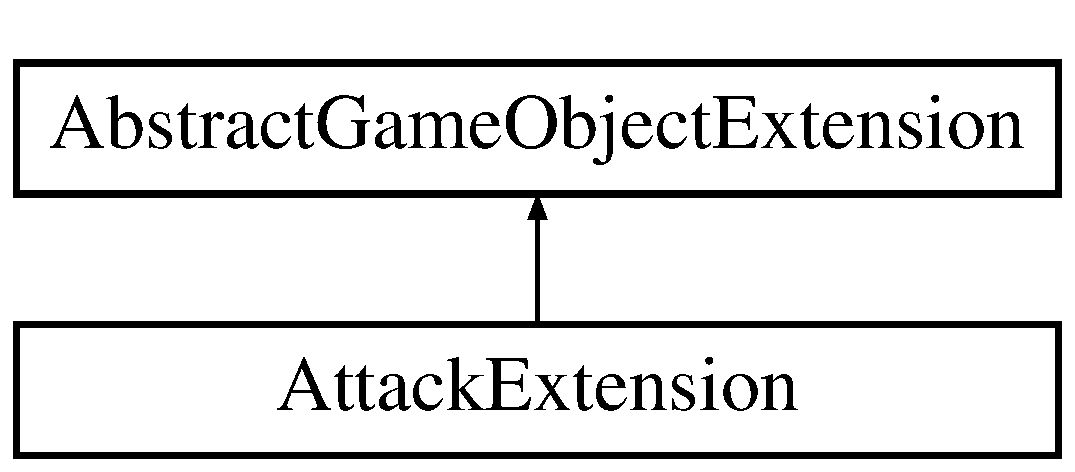
\includegraphics[height=2.000000cm]{class_attack_extension}
\end{center}
\end{figure}
\subsection*{Static Public Member Functions}
\begin{DoxyCompactItemize}
\item 
\mbox{\Hypertarget{class_attack_extension_ae1d31cc1bfefd2efe92475978b1a071c}\label{class_attack_extension_ae1d31cc1bfefd2efe92475978b1a071c}} 
static \mbox{\hyperlink{class_abstract_game_object_extension}{Abstract\+Game\+Object\+Extension}} $\ast$\+\_\+\+\_\+stdcall {\bfseries create} ()
\end{DoxyCompactItemize}
\subsection*{Additional Inherited Members}


The documentation for this class was generated from the following files\+:\begin{DoxyCompactItemize}
\item 
Attack\+Extension.\+h\item 
Attack\+Extension.\+cpp\end{DoxyCompactItemize}

\hypertarget{class_behaviour_attack}{}\section{Behaviour\+Attack Class Reference}
\label{class_behaviour_attack}\index{Behaviour\+Attack@{Behaviour\+Attack}}


Attack behavior  




{\ttfamily \#include $<$Behaviour\+Attack.\+h$>$}

Inheritance diagram for Behaviour\+Attack\+:\begin{figure}[H]
\begin{center}
\leavevmode
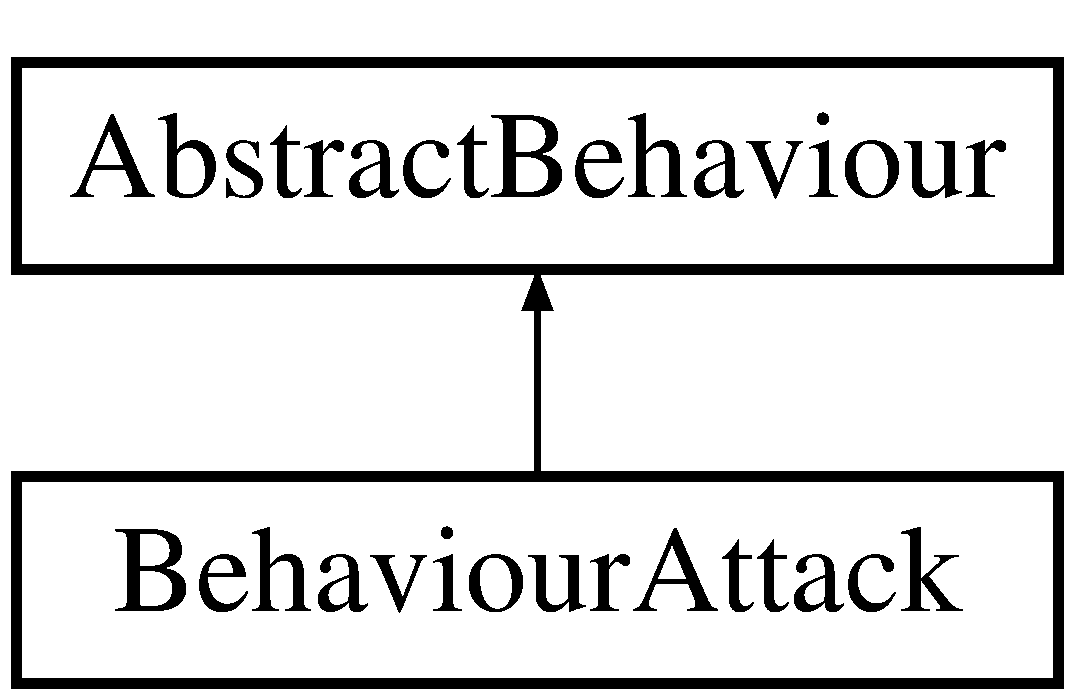
\includegraphics[height=2.000000cm]{class_behaviour_attack}
\end{center}
\end{figure}
\subsection*{Public Member Functions}
\begin{DoxyCompactItemize}
\item 
void \mbox{\hyperlink{class_behaviour_attack_aca669f46a6d32e5e41e7b477be1ee4cf}{execute}} ()
\begin{DoxyCompactList}\small\item\em Execute the behaviour. \end{DoxyCompactList}\item 
bool \mbox{\hyperlink{class_behaviour_attack_a539f70f642f0b21a808631fc64fbf2d8}{can\+Attack}} ()
\begin{DoxyCompactList}\small\item\em See if the object can be attacked. \end{DoxyCompactList}\item 
\mbox{\Hypertarget{class_behaviour_attack_a8a3a9217b3179f949a1d6a32f340c00c}\label{class_behaviour_attack_a8a3a9217b3179f949a1d6a32f340c00c}} 
{\bfseries Abstract\+Behaviour} (shared\+\_\+ptr$<$ \mbox{\hyperlink{class_game_object}{Game\+Object}} $>$ self, shared\+\_\+ptr$<$ vector$<$ \mbox{\hyperlink{class_game_object}{Game\+Object}} $>$$>$ scene)
\end{DoxyCompactItemize}
\subsection*{Additional Inherited Members}


\subsection{Detailed Description}
Attack behavior 



\subsection{Member Function Documentation}
\mbox{\Hypertarget{class_behaviour_attack_a539f70f642f0b21a808631fc64fbf2d8}\label{class_behaviour_attack_a539f70f642f0b21a808631fc64fbf2d8}} 
\index{Behaviour\+Attack@{Behaviour\+Attack}!can\+Attack@{can\+Attack}}
\index{can\+Attack@{can\+Attack}!Behaviour\+Attack@{Behaviour\+Attack}}
\subsubsection{\texorpdfstring{can\+Attack()}{canAttack()}}
{\footnotesize\ttfamily bool Behaviour\+Attack\+::can\+Attack (\begin{DoxyParamCaption}{ }\end{DoxyParamCaption})}



See if the object can be attacked. 

\begin{DoxyReturn}{Returns}
Can the object be attacked.
\end{DoxyReturn}
\mbox{\Hypertarget{class_behaviour_attack_aca669f46a6d32e5e41e7b477be1ee4cf}\label{class_behaviour_attack_aca669f46a6d32e5e41e7b477be1ee4cf}} 
\index{Behaviour\+Attack@{Behaviour\+Attack}!execute@{execute}}
\index{execute@{execute}!Behaviour\+Attack@{Behaviour\+Attack}}
\subsubsection{\texorpdfstring{execute()}{execute()}}
{\footnotesize\ttfamily void Behaviour\+Attack\+::execute (\begin{DoxyParamCaption}{ }\end{DoxyParamCaption})\hspace{0.3cm}{\ttfamily [virtual]}}



Execute the behaviour. 



Implements \mbox{\hyperlink{class_abstract_behaviour_ab99fb55a3b001e759e24d5b9721a742f}{Abstract\+Behaviour}}.



The documentation for this class was generated from the following files\+:\begin{DoxyCompactItemize}
\item 
Behaviour\+Attack.\+h\item 
Behaviour\+Attack.\+cpp\end{DoxyCompactItemize}

\hypertarget{class_behaviour_idle}{}\section{Behaviour\+Idle Class Reference}
\label{class_behaviour_idle}\index{Behaviour\+Idle@{Behaviour\+Idle}}


Idle ai behavior  




{\ttfamily \#include $<$Behaviour\+Idle.\+h$>$}

Inheritance diagram for Behaviour\+Idle\+:\begin{figure}[H]
\begin{center}
\leavevmode
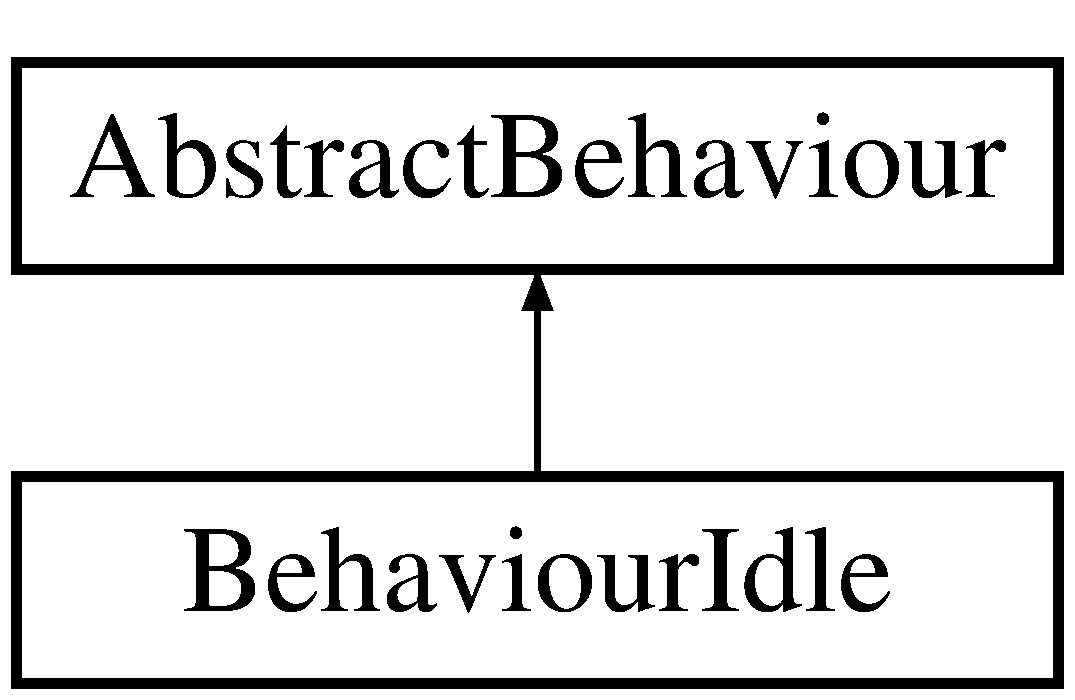
\includegraphics[height=2.000000cm]{class_behaviour_idle}
\end{center}
\end{figure}
\subsection*{Public Member Functions}
\begin{DoxyCompactItemize}
\item 
\mbox{\Hypertarget{class_behaviour_idle_ac810c315b1ea41772060b216ecdc2e11}\label{class_behaviour_idle_ac810c315b1ea41772060b216ecdc2e11}} 
void {\bfseries execute} ()
\item 
\mbox{\Hypertarget{class_behaviour_idle_a8a3a9217b3179f949a1d6a32f340c00c}\label{class_behaviour_idle_a8a3a9217b3179f949a1d6a32f340c00c}} 
{\bfseries Abstract\+Behaviour} (shared\+\_\+ptr$<$ \mbox{\hyperlink{class_game_object}{Game\+Object}} $>$ self, shared\+\_\+ptr$<$ vector$<$ \mbox{\hyperlink{class_game_object}{Game\+Object}} $>$$>$ scene)
\end{DoxyCompactItemize}
\subsection*{Additional Inherited Members}


\subsection{Detailed Description}
Idle ai behavior 



The documentation for this class was generated from the following files\+:\begin{DoxyCompactItemize}
\item 
Behaviour\+Idle.\+h\item 
Behaviour\+Idle.\+cpp\end{DoxyCompactItemize}

\hypertarget{class_behaviour_move}{}\section{Behaviour\+Move Class Reference}
\label{class_behaviour_move}\index{Behaviour\+Move@{Behaviour\+Move}}


Move ai behavior  




{\ttfamily \#include $<$Behaviour\+Move.\+h$>$}

Inheritance diagram for Behaviour\+Move\+:\begin{figure}[H]
\begin{center}
\leavevmode
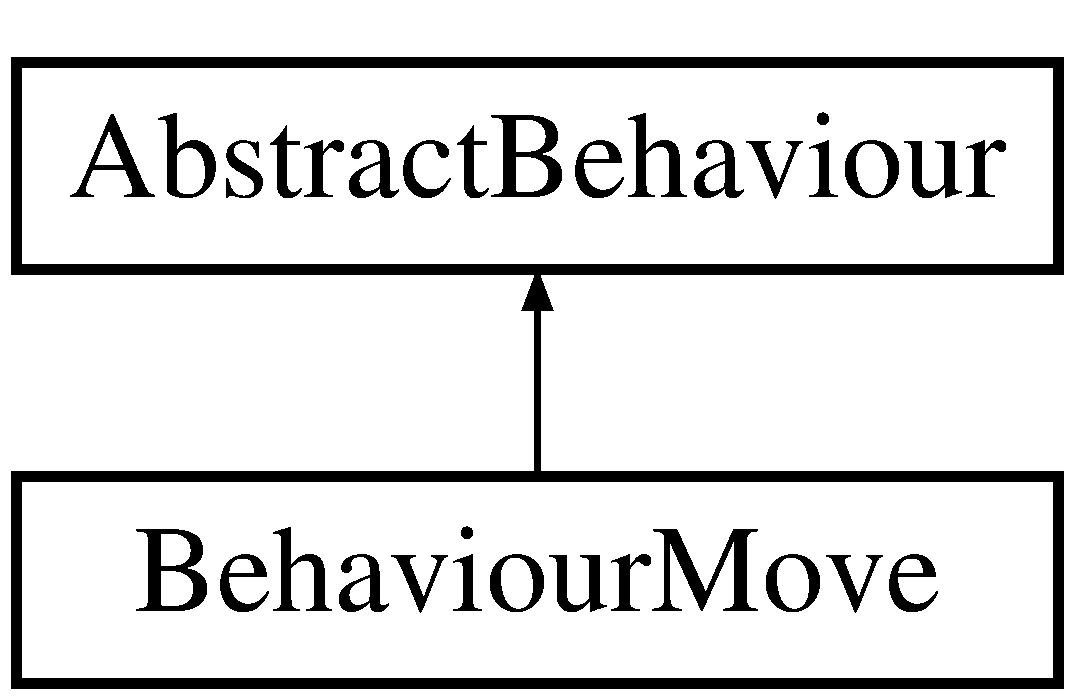
\includegraphics[height=2.000000cm]{class_behaviour_move}
\end{center}
\end{figure}
\subsection*{Public Member Functions}
\begin{DoxyCompactItemize}
\item 
\mbox{\Hypertarget{class_behaviour_move_a4cccd6dbe5ccf37b1522fc71a807f080}\label{class_behaviour_move_a4cccd6dbe5ccf37b1522fc71a807f080}} 
void {\bfseries execute} ()
\item 
\mbox{\Hypertarget{class_behaviour_move_a3d4182913183e85af80a1eba69a457a1}\label{class_behaviour_move_a3d4182913183e85af80a1eba69a457a1}} 
bool {\bfseries is\+Movable} ()
\item 
\mbox{\Hypertarget{class_behaviour_move_aebfd734f768321735b20f4e66ea1faab}\label{class_behaviour_move_aebfd734f768321735b20f4e66ea1faab}} 
bool {\bfseries is\+Wall\+Hit} ()
\item 
\mbox{\Hypertarget{class_behaviour_move_a8a3a9217b3179f949a1d6a32f340c00c}\label{class_behaviour_move_a8a3a9217b3179f949a1d6a32f340c00c}} 
{\bfseries Abstract\+Behaviour} (shared\+\_\+ptr$<$ \mbox{\hyperlink{class_game_object}{Game\+Object}} $>$ self, shared\+\_\+ptr$<$ vector$<$ \mbox{\hyperlink{class_game_object}{Game\+Object}} $>$$>$ scene)
\end{DoxyCompactItemize}
\subsection*{Additional Inherited Members}


\subsection{Detailed Description}
Move ai behavior 



The documentation for this class was generated from the following files\+:\begin{DoxyCompactItemize}
\item 
Behaviour\+Move.\+h\item 
Behaviour\+Move.\+cpp\end{DoxyCompactItemize}

\hypertarget{class_behaviour_rotate}{}\section{Behaviour\+Rotate Class Reference}
\label{class_behaviour_rotate}\index{Behaviour\+Rotate@{Behaviour\+Rotate}}


Rotate ai behavior  




{\ttfamily \#include $<$Behaviour\+Rotate.\+h$>$}

Inheritance diagram for Behaviour\+Rotate\+:\begin{figure}[H]
\begin{center}
\leavevmode
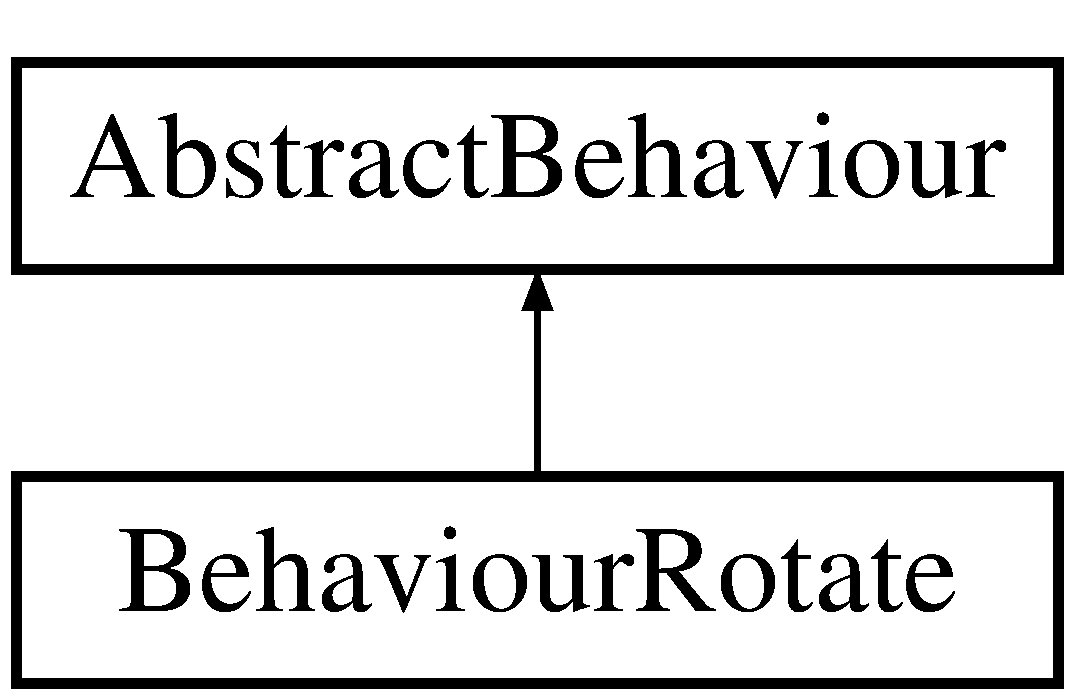
\includegraphics[height=2.000000cm]{class_behaviour_rotate}
\end{center}
\end{figure}
\subsection*{Public Member Functions}
\begin{DoxyCompactItemize}
\item 
void \mbox{\hyperlink{class_behaviour_rotate_aa01153f4a487813580ecb5d5145da47c}{execute}} ()
\begin{DoxyCompactList}\small\item\em Execute the behaviour. \end{DoxyCompactList}\item 
bool \mbox{\hyperlink{class_behaviour_rotate_a35e30578ca4a2a7fd96e01573e5791fd}{has\+Enough\+Time\+Elapsed}} ()
\begin{DoxyCompactList}\small\item\em If enough time has elapsed for the next rotation. \end{DoxyCompactList}\item 
bool \mbox{\hyperlink{class_behaviour_rotate_a93f1ef9eb3fe2ea8dfb49a4e435b48a5}{can\+Rotate}} ()
\begin{DoxyCompactList}\small\item\em Looks if the object can be rotated. \end{DoxyCompactList}\item 
\mbox{\Hypertarget{class_behaviour_rotate_a8a3a9217b3179f949a1d6a32f340c00c}\label{class_behaviour_rotate_a8a3a9217b3179f949a1d6a32f340c00c}} 
{\bfseries Abstract\+Behaviour} (shared\+\_\+ptr$<$ \mbox{\hyperlink{class_game_object}{Game\+Object}} $>$ self, shared\+\_\+ptr$<$ vector$<$ \mbox{\hyperlink{class_game_object}{Game\+Object}} $>$$>$ scene)
\end{DoxyCompactItemize}
\subsection*{Additional Inherited Members}


\subsection{Detailed Description}
Rotate ai behavior 



\subsection{Member Function Documentation}
\mbox{\Hypertarget{class_behaviour_rotate_a93f1ef9eb3fe2ea8dfb49a4e435b48a5}\label{class_behaviour_rotate_a93f1ef9eb3fe2ea8dfb49a4e435b48a5}} 
\index{Behaviour\+Rotate@{Behaviour\+Rotate}!can\+Rotate@{can\+Rotate}}
\index{can\+Rotate@{can\+Rotate}!Behaviour\+Rotate@{Behaviour\+Rotate}}
\subsubsection{\texorpdfstring{can\+Rotate()}{canRotate()}}
{\footnotesize\ttfamily bool Behaviour\+Rotate\+::can\+Rotate (\begin{DoxyParamCaption}{ }\end{DoxyParamCaption})}



Looks if the object can be rotated. 

\begin{DoxyReturn}{Returns}
If the object can be rotated
\end{DoxyReturn}
\mbox{\Hypertarget{class_behaviour_rotate_aa01153f4a487813580ecb5d5145da47c}\label{class_behaviour_rotate_aa01153f4a487813580ecb5d5145da47c}} 
\index{Behaviour\+Rotate@{Behaviour\+Rotate}!execute@{execute}}
\index{execute@{execute}!Behaviour\+Rotate@{Behaviour\+Rotate}}
\subsubsection{\texorpdfstring{execute()}{execute()}}
{\footnotesize\ttfamily void Behaviour\+Rotate\+::execute (\begin{DoxyParamCaption}{ }\end{DoxyParamCaption})\hspace{0.3cm}{\ttfamily [virtual]}}



Execute the behaviour. 



Implements \mbox{\hyperlink{class_abstract_behaviour_ab99fb55a3b001e759e24d5b9721a742f}{Abstract\+Behaviour}}.

\mbox{\Hypertarget{class_behaviour_rotate_a35e30578ca4a2a7fd96e01573e5791fd}\label{class_behaviour_rotate_a35e30578ca4a2a7fd96e01573e5791fd}} 
\index{Behaviour\+Rotate@{Behaviour\+Rotate}!has\+Enough\+Time\+Elapsed@{has\+Enough\+Time\+Elapsed}}
\index{has\+Enough\+Time\+Elapsed@{has\+Enough\+Time\+Elapsed}!Behaviour\+Rotate@{Behaviour\+Rotate}}
\subsubsection{\texorpdfstring{has\+Enough\+Time\+Elapsed()}{hasEnoughTimeElapsed()}}
{\footnotesize\ttfamily bool Behaviour\+Rotate\+::has\+Enough\+Time\+Elapsed (\begin{DoxyParamCaption}{ }\end{DoxyParamCaption})}



If enough time has elapsed for the next rotation. 

\begin{DoxyReturn}{Returns}
If enough time has elapsed
\end{DoxyReturn}


The documentation for this class was generated from the following files\+:\begin{DoxyCompactItemize}
\item 
Behaviour\+Rotate.\+h\item 
Behaviour\+Rotate.\+cpp\end{DoxyCompactItemize}

\hypertarget{class_behaviour_sees_enemy}{}\section{Behaviour\+Sees\+Enemy Class Reference}
\label{class_behaviour_sees_enemy}\index{Behaviour\+Sees\+Enemy@{Behaviour\+Sees\+Enemy}}


Sees enemy ai behavior  




{\ttfamily \#include $<$Behaviour\+Sees\+Enemy.\+h$>$}

Inheritance diagram for Behaviour\+Sees\+Enemy\+:\begin{figure}[H]
\begin{center}
\leavevmode
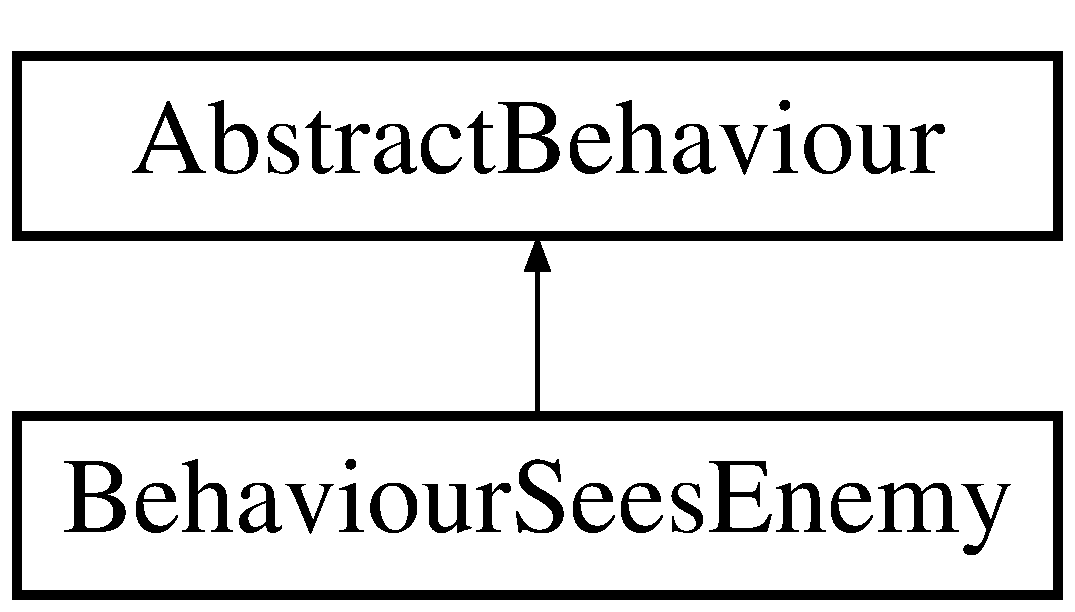
\includegraphics[height=2.000000cm]{class_behaviour_sees_enemy}
\end{center}
\end{figure}
\subsection*{Public Member Functions}
\begin{DoxyCompactItemize}
\item 
void \mbox{\hyperlink{class_behaviour_sees_enemy_afddbf2ca7396c9fd7b24f4be60edb84c}{execute}} ()
\begin{DoxyCompactList}\small\item\em Execute the behaviour. \end{DoxyCompactList}\item 
\mbox{\Hypertarget{class_behaviour_sees_enemy_a8a3a9217b3179f949a1d6a32f340c00c}\label{class_behaviour_sees_enemy_a8a3a9217b3179f949a1d6a32f340c00c}} 
{\bfseries Abstract\+Behaviour} (shared\+\_\+ptr$<$ \mbox{\hyperlink{class_game_object}{Game\+Object}} $>$ self, shared\+\_\+ptr$<$ vector$<$ \mbox{\hyperlink{class_game_object}{Game\+Object}} $>$$>$ scene)
\end{DoxyCompactItemize}
\subsection*{Additional Inherited Members}


\subsection{Detailed Description}
Sees enemy ai behavior 



\subsection{Member Function Documentation}
\mbox{\Hypertarget{class_behaviour_sees_enemy_afddbf2ca7396c9fd7b24f4be60edb84c}\label{class_behaviour_sees_enemy_afddbf2ca7396c9fd7b24f4be60edb84c}} 
\index{Behaviour\+Sees\+Enemy@{Behaviour\+Sees\+Enemy}!execute@{execute}}
\index{execute@{execute}!Behaviour\+Sees\+Enemy@{Behaviour\+Sees\+Enemy}}
\subsubsection{\texorpdfstring{execute()}{execute()}}
{\footnotesize\ttfamily void Behaviour\+Sees\+Enemy\+::execute (\begin{DoxyParamCaption}{ }\end{DoxyParamCaption})\hspace{0.3cm}{\ttfamily [virtual]}}



Execute the behaviour. 



Implements \mbox{\hyperlink{class_abstract_behaviour_ab99fb55a3b001e759e24d5b9721a742f}{Abstract\+Behaviour}}.



The documentation for this class was generated from the following files\+:\begin{DoxyCompactItemize}
\item 
Behaviour\+Sees\+Enemy.\+h\item 
Behaviour\+Sees\+Enemy.\+cpp\end{DoxyCompactItemize}

\hypertarget{struct_body}{}\section{Body Struct Reference}
\label{struct_body}\index{Body@{Body}}
\subsection*{Public Attributes}
\begin{DoxyCompactItemize}
\item 
\mbox{\Hypertarget{struct_body_a659001c4570d0ad46bf609ab06447860}\label{struct_body_a659001c4570d0ad46bf609ab06447860}} 
\mbox{\hyperlink{struct_vec2}{Vec2}} {\bfseries position}
\item 
\mbox{\Hypertarget{struct_body_a3723eaa2db4c9a3ac68b9745e11a0a40}\label{struct_body_a3723eaa2db4c9a3ac68b9745e11a0a40}} 
\mbox{\hyperlink{struct_vec2}{Vec2}} {\bfseries velocity}
\item 
\mbox{\Hypertarget{struct_body_a78f0f4d1c6a6b9efaefd5a03bd8de598}\label{struct_body_a78f0f4d1c6a6b9efaefd5a03bd8de598}} 
real {\bfseries angular\+Velocity}
\item 
\mbox{\Hypertarget{struct_body_a269761d1be497882d3f3a2aef4847152}\label{struct_body_a269761d1be497882d3f3a2aef4847152}} 
real {\bfseries torque}
\item 
\mbox{\Hypertarget{struct_body_a93534f084248dd60be496754361c1a22}\label{struct_body_a93534f084248dd60be496754361c1a22}} 
real {\bfseries orient}
\item 
\mbox{\Hypertarget{struct_body_a0399faa61bf3850a1dacb2ed3f377ba5}\label{struct_body_a0399faa61bf3850a1dacb2ed3f377ba5}} 
\mbox{\hyperlink{struct_vec2}{Vec2}} {\bfseries force}
\item 
\mbox{\Hypertarget{struct_body_a48ced797496c1cd5bf4175cfc16c2364}\label{struct_body_a48ced797496c1cd5bf4175cfc16c2364}} 
real {\bfseries I}
\item 
\mbox{\Hypertarget{struct_body_abab39f15217fc548e93a27eeda630c20}\label{struct_body_abab39f15217fc548e93a27eeda630c20}} 
real {\bfseries iI}
\item 
\mbox{\Hypertarget{struct_body_abbf210246f192562bf8809f2b2c3e238}\label{struct_body_abbf210246f192562bf8809f2b2c3e238}} 
real {\bfseries m}
\item 
\mbox{\Hypertarget{struct_body_a500c28fac5382a812430a095f35d355f}\label{struct_body_a500c28fac5382a812430a095f35d355f}} 
real {\bfseries im}
\item 
\mbox{\Hypertarget{struct_body_aa57d627e73de706e87540b07b61d867a}\label{struct_body_aa57d627e73de706e87540b07b61d867a}} 
real {\bfseries restitution}
\end{DoxyCompactItemize}


The documentation for this struct was generated from the following file\+:\begin{DoxyCompactItemize}
\item 
Body.\+h\end{DoxyCompactItemize}

\hypertarget{class_button_ui_element}{}\section{Button\+Ui\+Element Class Reference}
\label{class_button_ui_element}\index{Button\+Ui\+Element@{Button\+Ui\+Element}}


Button element  




{\ttfamily \#include $<$Button\+Ui\+Element.\+h$>$}

Inheritance diagram for Button\+Ui\+Element\+:\begin{figure}[H]
\begin{center}
\leavevmode
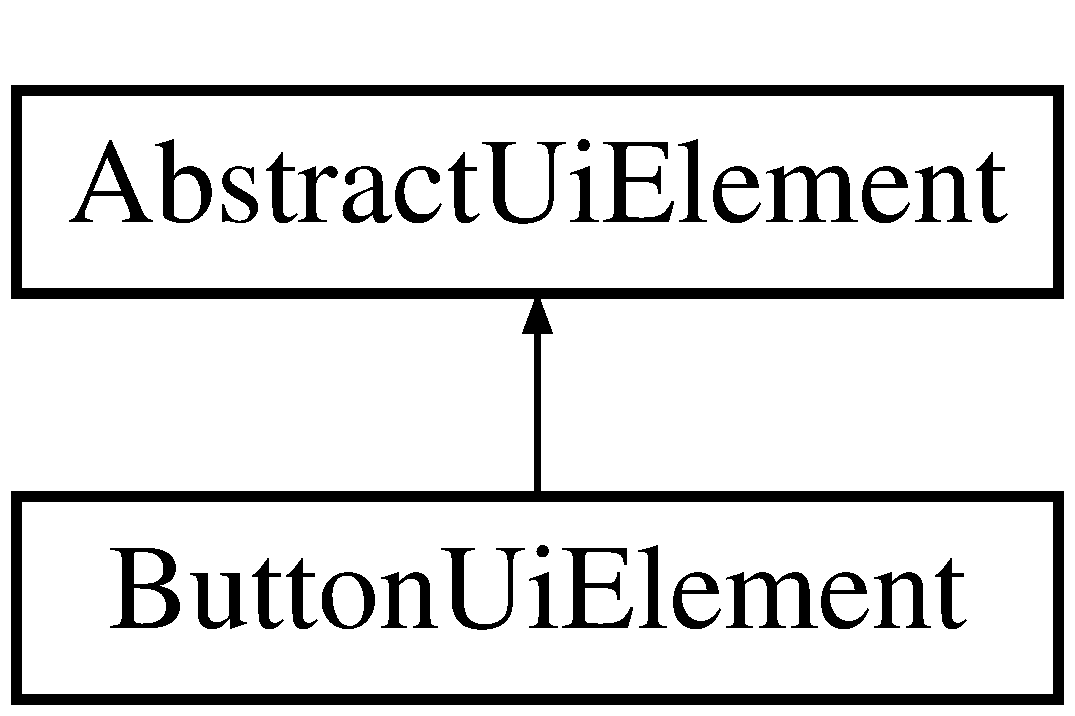
\includegraphics[height=2.000000cm]{class_button_ui_element}
\end{center}
\end{figure}
\subsection*{Public Member Functions}
\begin{DoxyCompactItemize}
\item 
\mbox{\Hypertarget{class_button_ui_element_abbc16623af7c8c568f99689dafd4dc0f}\label{class_button_ui_element_abbc16623af7c8c568f99689dafd4dc0f}} 
{\bfseries Button\+Ui\+Element} (std\+::string text, \mbox{\hyperlink{struct_rect}{Rect}} rect, \mbox{\hyperlink{struct_color}{Color}} bg\+Color, \mbox{\hyperlink{struct_color}{Color}} fg\+Color, std\+::string font\+Key, int font\+Size)
\item 
void \mbox{\hyperlink{class_button_ui_element_a035c8beddc1ff6d47b94953025f68422}{pre\+Render}} (\mbox{\hyperlink{class_window}{Window}} $\ast$window)
\item 
void \mbox{\hyperlink{class_button_ui_element_ad97fc68e9279a36182c66b07dfa28817}{render}} (\mbox{\hyperlink{class_window}{Window}} $\ast$window)
\begin{DoxyCompactList}\small\item\em Render the element on the screen. \end{DoxyCompactList}\item 
void \mbox{\hyperlink{class_button_ui_element_a06c748ef9e81216f76d7db936d320365}{on\+Click}} ()
\begin{DoxyCompactList}\small\item\em The function executed when the element is clicked on. \end{DoxyCompactList}\item 
bool \mbox{\hyperlink{class_button_ui_element_ab321d646770df66f7ea58a7246d7bf28}{is\+In\+Bound}} (int mouseX, int mouseY)
\begin{DoxyCompactList}\small\item\em Checks if the mouse is within the bounds of the element. \end{DoxyCompactList}\item 
\mbox{\Hypertarget{class_button_ui_element_a24799afea36fcb1135b9477f1da3498d}\label{class_button_ui_element_a24799afea36fcb1135b9477f1da3498d}} 
{\bfseries Abstract\+Ui\+Element} ()
\end{DoxyCompactItemize}
\subsection*{Additional Inherited Members}


\subsection{Detailed Description}
Button element 



\subsection{Member Function Documentation}
\mbox{\Hypertarget{class_button_ui_element_ab321d646770df66f7ea58a7246d7bf28}\label{class_button_ui_element_ab321d646770df66f7ea58a7246d7bf28}} 
\index{Button\+Ui\+Element@{Button\+Ui\+Element}!is\+In\+Bound@{is\+In\+Bound}}
\index{is\+In\+Bound@{is\+In\+Bound}!Button\+Ui\+Element@{Button\+Ui\+Element}}
\subsubsection{\texorpdfstring{is\+In\+Bound()}{isInBound()}}
{\footnotesize\ttfamily bool Button\+Ui\+Element\+::is\+In\+Bound (\begin{DoxyParamCaption}\item[{int}]{mouseX,  }\item[{int}]{mouseY }\end{DoxyParamCaption})\hspace{0.3cm}{\ttfamily [virtual]}}



Checks if the mouse is within the bounds of the element. 


\begin{DoxyParams}{Parameters}
{\em mouseX} & X coordinate of the mouse\\
\hline
{\em mouseY} & Y coordinate of the mouse\\
\hline
\end{DoxyParams}
\begin{DoxyReturn}{Returns}

\end{DoxyReturn}


Implements \mbox{\hyperlink{class_abstract_ui_element_ad2c415461cd7e8c1ee50b1105eb84685}{Abstract\+Ui\+Element}}.

\mbox{\Hypertarget{class_button_ui_element_a06c748ef9e81216f76d7db936d320365}\label{class_button_ui_element_a06c748ef9e81216f76d7db936d320365}} 
\index{Button\+Ui\+Element@{Button\+Ui\+Element}!on\+Click@{on\+Click}}
\index{on\+Click@{on\+Click}!Button\+Ui\+Element@{Button\+Ui\+Element}}
\subsubsection{\texorpdfstring{on\+Click()}{onClick()}}
{\footnotesize\ttfamily void Button\+Ui\+Element\+::on\+Click (\begin{DoxyParamCaption}{ }\end{DoxyParamCaption})\hspace{0.3cm}{\ttfamily [virtual]}}



The function executed when the element is clicked on. 



Implements \mbox{\hyperlink{class_abstract_ui_element_a42296c15c9e70b6ac7fda0b1862612af}{Abstract\+Ui\+Element}}.

\mbox{\Hypertarget{class_button_ui_element_a035c8beddc1ff6d47b94953025f68422}\label{class_button_ui_element_a035c8beddc1ff6d47b94953025f68422}} 
\index{Button\+Ui\+Element@{Button\+Ui\+Element}!pre\+Render@{pre\+Render}}
\index{pre\+Render@{pre\+Render}!Button\+Ui\+Element@{Button\+Ui\+Element}}
\subsubsection{\texorpdfstring{pre\+Render()}{preRender()}}
{\footnotesize\ttfamily void Button\+Ui\+Element\+::pre\+Render (\begin{DoxyParamCaption}\item[{\mbox{\hyperlink{class_window}{Window}} $\ast$}]{window }\end{DoxyParamCaption})\hspace{0.3cm}{\ttfamily [virtual]}}

This is called one time before going into the render loop. 


\begin{DoxyParams}{Parameters}
{\em renderer} & The renderer\\
\hline
\end{DoxyParams}


Implements \mbox{\hyperlink{class_abstract_ui_element_a859f627ab385e9d3bf6ce8db40607cdb}{Abstract\+Ui\+Element}}.

\mbox{\Hypertarget{class_button_ui_element_ad97fc68e9279a36182c66b07dfa28817}\label{class_button_ui_element_ad97fc68e9279a36182c66b07dfa28817}} 
\index{Button\+Ui\+Element@{Button\+Ui\+Element}!render@{render}}
\index{render@{render}!Button\+Ui\+Element@{Button\+Ui\+Element}}
\subsubsection{\texorpdfstring{render()}{render()}}
{\footnotesize\ttfamily void Button\+Ui\+Element\+::render (\begin{DoxyParamCaption}\item[{\mbox{\hyperlink{class_window}{Window}} $\ast$}]{window }\end{DoxyParamCaption})\hspace{0.3cm}{\ttfamily [virtual]}}



Render the element on the screen. 


\begin{DoxyParams}{Parameters}
{\em renderer} & The renderer\\
\hline
\end{DoxyParams}


Implements \mbox{\hyperlink{class_abstract_ui_element_aea66ce333323cf2d5e12d4de9515de7b}{Abstract\+Ui\+Element}}.



The documentation for this class was generated from the following files\+:\begin{DoxyCompactItemize}
\item 
Button\+Ui\+Element.\+h\item 
Button\+Ui\+Element.\+cpp\end{DoxyCompactItemize}

\hypertarget{class_can_wield_extension}{}\section{Can\+Wield\+Extension Class Reference}
\label{class_can_wield_extension}\index{Can\+Wield\+Extension@{Can\+Wield\+Extension}}
Inheritance diagram for Can\+Wield\+Extension\+:\begin{figure}[H]
\begin{center}
\leavevmode
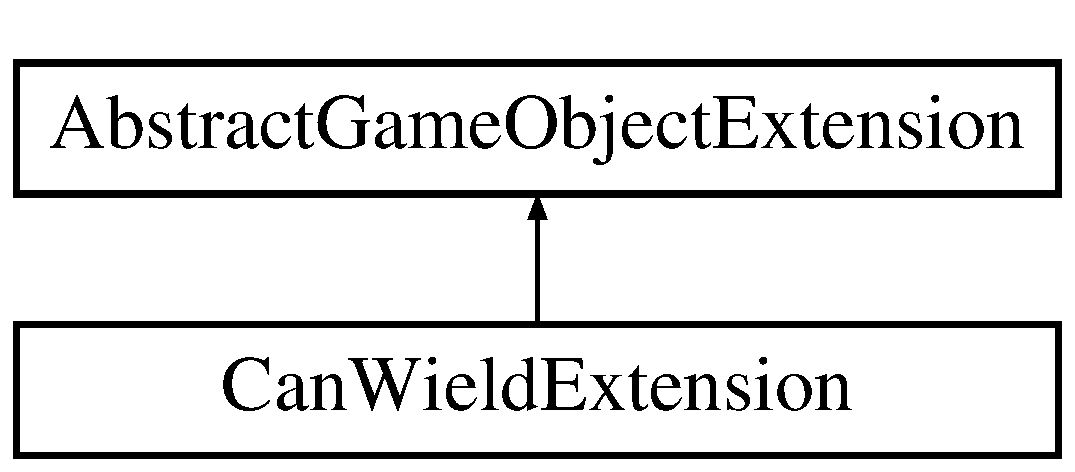
\includegraphics[height=2.000000cm]{class_can_wield_extension}
\end{center}
\end{figure}
\subsection*{Public Member Functions}
\begin{DoxyCompactItemize}
\item 
\mbox{\Hypertarget{class_can_wield_extension_a1ffe84dc23c27890b0efcf0fc5aa43a0}\label{class_can_wield_extension_a1ffe84dc23c27890b0efcf0fc5aa43a0}} 
void {\bfseries add\+Item} (\mbox{\hyperlink{class_abstract_manageable_item}{Abstract\+Manageable\+Item}})
\item 
\mbox{\Hypertarget{class_can_wield_extension_a49c43410be01b7504ff4f9af9ee43459}\label{class_can_wield_extension_a49c43410be01b7504ff4f9af9ee43459}} 
void {\bfseries remove\+Item} (\mbox{\hyperlink{class_abstract_manageable_item}{Abstract\+Manageable\+Item}})
\end{DoxyCompactItemize}
\subsection*{Static Public Member Functions}
\begin{DoxyCompactItemize}
\item 
\mbox{\Hypertarget{class_can_wield_extension_abd3f9d8c241cf152f8118872301f318f}\label{class_can_wield_extension_abd3f9d8c241cf152f8118872301f318f}} 
static \mbox{\hyperlink{class_abstract_game_object_extension}{Abstract\+Game\+Object\+Extension}} $\ast$\+\_\+\+\_\+stdcall {\bfseries create} ()
\end{DoxyCompactItemize}
\subsection*{Additional Inherited Members}


The documentation for this class was generated from the following files\+:\begin{DoxyCompactItemize}
\item 
Can\+Wield\+Extension.\+h\item 
Can\+Wield\+Extension.\+cpp\end{DoxyCompactItemize}

\hypertarget{class_check_physics_extension}{}\section{Check\+Physics\+Extension Class Reference}
\label{class_check_physics_extension}\index{Check\+Physics\+Extension@{Check\+Physics\+Extension}}


\mbox{\hyperlink{class_physics}{Physics}}  




{\ttfamily \#include $<$Check\+Physics\+Extension.\+h$>$}

Inheritance diagram for Check\+Physics\+Extension\+:\begin{figure}[H]
\begin{center}
\leavevmode
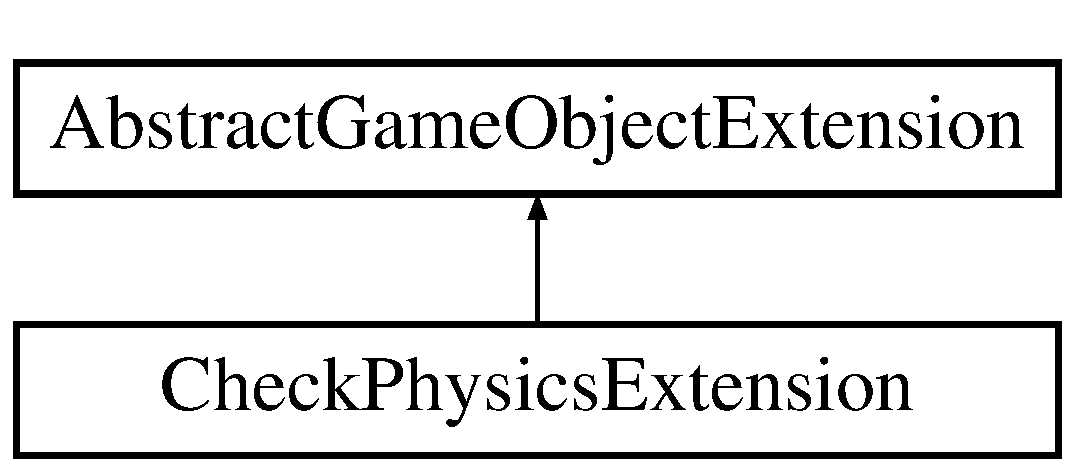
\includegraphics[height=2.000000cm]{class_check_physics_extension}
\end{center}
\end{figure}
\subsection*{Public Member Functions}
\begin{DoxyCompactItemize}
\item 
\mbox{\Hypertarget{class_check_physics_extension_a8a830590dbc7f53e3a785a630b6e285c}\label{class_check_physics_extension_a8a830590dbc7f53e3a785a630b6e285c}} 
void {\bfseries do\+Physics} (vector$<$ shared\+\_\+ptr$<$ \mbox{\hyperlink{class_game_object}{Game\+Object}} $>$$>$ game\+Object\+List)
\end{DoxyCompactItemize}
\subsection*{Static Public Member Functions}
\begin{DoxyCompactItemize}
\item 
\mbox{\Hypertarget{class_check_physics_extension_a09d2a0a0e848825c71f044350058530e}\label{class_check_physics_extension_a09d2a0a0e848825c71f044350058530e}} 
static \mbox{\hyperlink{class_abstract_game_object_extension}{Abstract\+Game\+Object\+Extension}} $\ast$\+\_\+\+\_\+stdcall {\bfseries create} ()
\end{DoxyCompactItemize}
\subsection*{Additional Inherited Members}


\subsection{Detailed Description}
\mbox{\hyperlink{class_physics}{Physics}} 



The documentation for this class was generated from the following files\+:\begin{DoxyCompactItemize}
\item 
Check\+Physics\+Extension.\+h\item 
Check\+Physics\+Extension.\+cpp\end{DoxyCompactItemize}

\hypertarget{class_collision}{}\section{Collision Class Reference}
\label{class_collision}\index{Collision@{Collision}}


\mbox{\hyperlink{class_collision}{Collision}} detection and resolution  




{\ttfamily \#include $<$Collision.\+h$>$}

\subsection*{Public Member Functions}
\begin{DoxyCompactItemize}
\item 
\mbox{\Hypertarget{class_collision_a326e71d8960461f00b118f1688f61e81}\label{class_collision_a326e71d8960461f00b118f1688f61e81}} 
std\+::vector$<$ shared\+\_\+ptr$<$ \mbox{\hyperlink{class_game_object}{Game\+Object}} $>$ $>$ {\bfseries get\+Collisions} (shared\+\_\+ptr$<$ \mbox{\hyperlink{class_game_object}{Game\+Object}} $>$ objectA, std\+::vector$<$ shared\+\_\+ptr$<$ \mbox{\hyperlink{class_game_object}{Game\+Object}} $>$$>$ object\+List)
\item 
void \mbox{\hyperlink{class_collision_a9af0ec7e3829efcec43bf94e5911f1ae}{resolve\+Collision}} (shared\+\_\+ptr$<$ \mbox{\hyperlink{class_game_object}{Game\+Object}} $>$ objectA, shared\+\_\+ptr$<$ \mbox{\hyperlink{class_game_object}{Game\+Object}} $>$ objectB)
\begin{DoxyCompactList}\small\item\em Resolve collision between 2 game objects. \end{DoxyCompactList}\end{DoxyCompactItemize}


\subsection{Detailed Description}
\mbox{\hyperlink{class_collision}{Collision}} detection and resolution 



\subsection{Member Function Documentation}
\mbox{\Hypertarget{class_collision_a9af0ec7e3829efcec43bf94e5911f1ae}\label{class_collision_a9af0ec7e3829efcec43bf94e5911f1ae}} 
\index{Collision@{Collision}!resolve\+Collision@{resolve\+Collision}}
\index{resolve\+Collision@{resolve\+Collision}!Collision@{Collision}}
\subsubsection{\texorpdfstring{resolve\+Collision()}{resolveCollision()}}
{\footnotesize\ttfamily void Collision\+::resolve\+Collision (\begin{DoxyParamCaption}\item[{shared\+\_\+ptr$<$ \mbox{\hyperlink{class_game_object}{Game\+Object}} $>$}]{objectA,  }\item[{shared\+\_\+ptr$<$ \mbox{\hyperlink{class_game_object}{Game\+Object}} $>$}]{objectB }\end{DoxyParamCaption})}



Resolve collision between 2 game objects. 


\begin{DoxyParams}{Parameters}
{\em objectA} & Game\+ObjectA\\
\hline
{\em objectB} & Game\+ObjectB\\
\hline
\end{DoxyParams}


The documentation for this class was generated from the following files\+:\begin{DoxyCompactItemize}
\item 
Collision.\+h\item 
Collision.\+cpp\end{DoxyCompactItemize}

\hypertarget{class_collision_resolution_default_extension}{}\section{Collision\+Resolution\+Default\+Extension Class Reference}
\label{class_collision_resolution_default_extension}\index{Collision\+Resolution\+Default\+Extension@{Collision\+Resolution\+Default\+Extension}}
Inheritance diagram for Collision\+Resolution\+Default\+Extension\+:\begin{figure}[H]
\begin{center}
\leavevmode
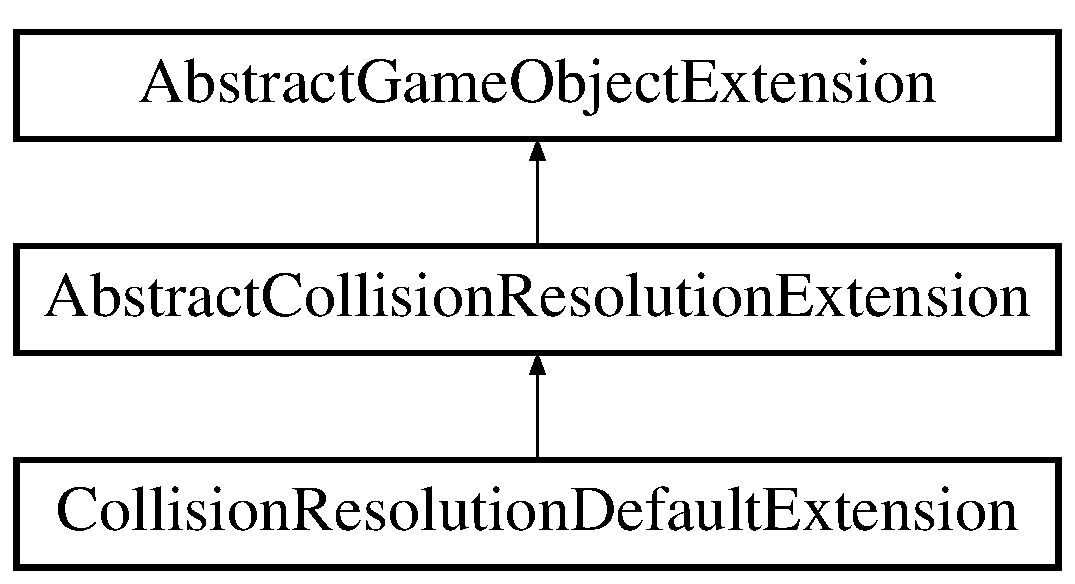
\includegraphics[height=3.000000cm]{class_collision_resolution_default_extension}
\end{center}
\end{figure}
\subsection*{Public Member Functions}
\begin{DoxyCompactItemize}
\item 
\mbox{\Hypertarget{class_collision_resolution_default_extension_a68069b51c3b8c07186313d33eb9c9f4e}\label{class_collision_resolution_default_extension_a68069b51c3b8c07186313d33eb9c9f4e}} 
bool {\bfseries is\+Default} ()
\item 
\mbox{\Hypertarget{class_collision_resolution_default_extension_ae5b4ea88f403a4deb68ac2de309df4aa}\label{class_collision_resolution_default_extension_ae5b4ea88f403a4deb68ac2de309df4aa}} 
void {\bfseries resolve\+Collision} (shared\+\_\+ptr$<$ \mbox{\hyperlink{class_game_object}{Game\+Object}} $>$ other\+Object)
\end{DoxyCompactItemize}
\subsection*{Static Public Member Functions}
\begin{DoxyCompactItemize}
\item 
\mbox{\Hypertarget{class_collision_resolution_default_extension_a6819e10299dd24e147b43971128a50f5}\label{class_collision_resolution_default_extension_a6819e10299dd24e147b43971128a50f5}} 
static \mbox{\hyperlink{class_abstract_game_object_extension}{Abstract\+Game\+Object\+Extension}} $\ast$\+\_\+\+\_\+stdcall {\bfseries create} ()
\end{DoxyCompactItemize}
\subsection*{Additional Inherited Members}


The documentation for this class was generated from the following files\+:\begin{DoxyCompactItemize}
\item 
Collision\+Resolution\+Default\+Extension.\+h\item 
Collision\+Resolution\+Default\+Extension.\+cpp\end{DoxyCompactItemize}

\hypertarget{class_collision_resolution_portal_extension}{}\section{Collision\+Resolution\+Portal\+Extension Class Reference}
\label{class_collision_resolution_portal_extension}\index{Collision\+Resolution\+Portal\+Extension@{Collision\+Resolution\+Portal\+Extension}}
Inheritance diagram for Collision\+Resolution\+Portal\+Extension\+:\begin{figure}[H]
\begin{center}
\leavevmode
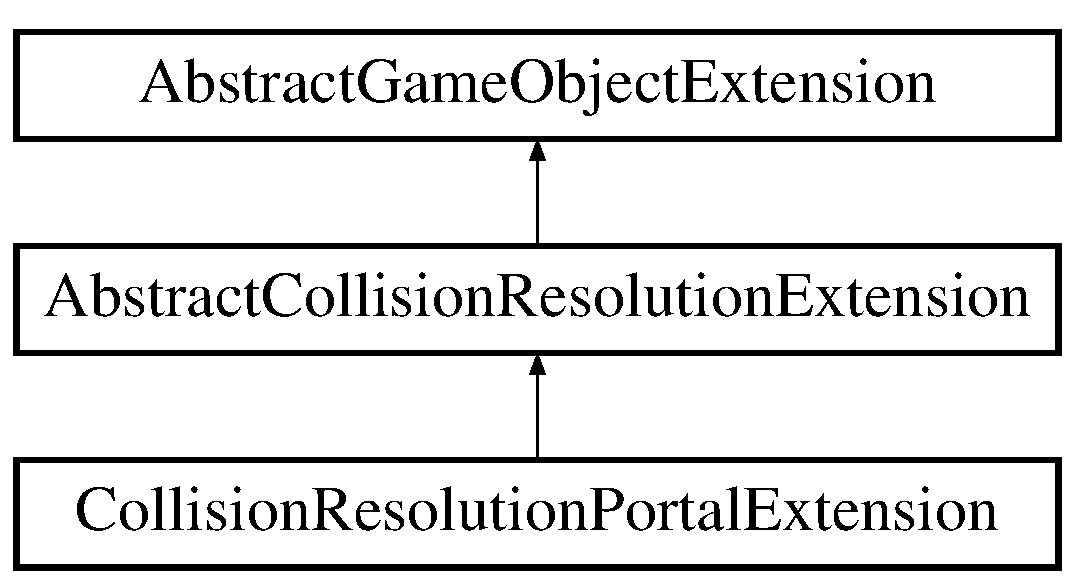
\includegraphics[height=3.000000cm]{class_collision_resolution_portal_extension}
\end{center}
\end{figure}
\subsection*{Public Member Functions}
\begin{DoxyCompactItemize}
\item 
\mbox{\Hypertarget{class_collision_resolution_portal_extension_a4bd3ee292b5a8bfd5b6fbb21175c2016}\label{class_collision_resolution_portal_extension_a4bd3ee292b5a8bfd5b6fbb21175c2016}} 
bool {\bfseries is\+Default} ()
\item 
\mbox{\Hypertarget{class_collision_resolution_portal_extension_a4e006318b6367308bd6be155211c8d9e}\label{class_collision_resolution_portal_extension_a4e006318b6367308bd6be155211c8d9e}} 
void {\bfseries resolve\+Collision} (shared\+\_\+ptr$<$ \mbox{\hyperlink{class_game_object}{Game\+Object}} $>$ other\+Object)
\end{DoxyCompactItemize}
\subsection*{Static Public Member Functions}
\begin{DoxyCompactItemize}
\item 
\mbox{\Hypertarget{class_collision_resolution_portal_extension_a8cf6352f6c005ddd81a170c5723b5adf}\label{class_collision_resolution_portal_extension_a8cf6352f6c005ddd81a170c5723b5adf}} 
static \mbox{\hyperlink{class_abstract_game_object_extension}{Abstract\+Game\+Object\+Extension}} $\ast$\+\_\+\+\_\+stdcall {\bfseries create} ()
\end{DoxyCompactItemize}
\subsection*{Additional Inherited Members}


The documentation for this class was generated from the following files\+:\begin{DoxyCompactItemize}
\item 
Collision\+Resolution\+Portal\+Extension.\+h\item 
Collision\+Resolution\+Portal\+Extension.\+cpp\end{DoxyCompactItemize}

\hypertarget{class_default_entity_a_i}{}\section{Default\+Entity\+AI Class Reference}
\label{class_default_entity_a_i}\index{Default\+Entity\+AI@{Default\+Entity\+AI}}
Inheritance diagram for Default\+Entity\+AI\+:\begin{figure}[H]
\begin{center}
\leavevmode
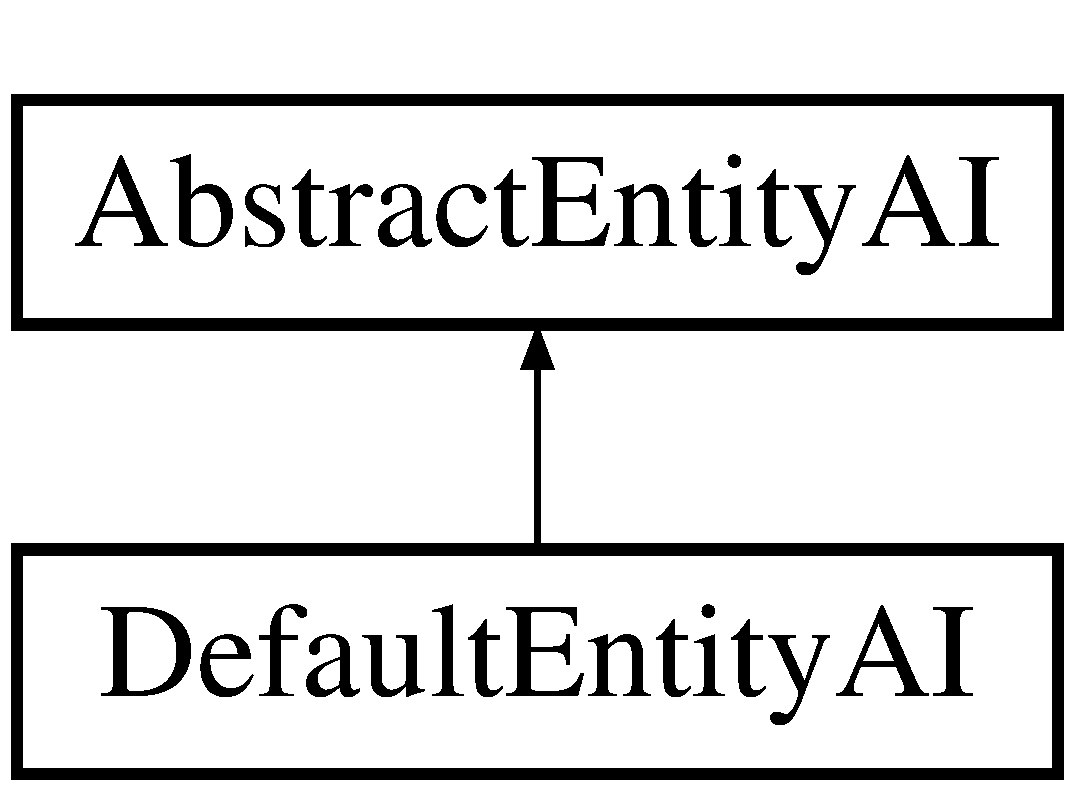
\includegraphics[height=2.000000cm]{class_default_entity_a_i}
\end{center}
\end{figure}
\subsection*{Public Member Functions}
\begin{DoxyCompactItemize}
\item 
void \mbox{\hyperlink{class_default_entity_a_i_a86fb7d0e18f1e3de4dd1fb3aea5acf84}{create\+Behaviour\+Tree}} (shared\+\_\+ptr$<$ \mbox{\hyperlink{class_game_object}{Game\+Object}} $>$ self, shared\+\_\+ptr$<$ vector$<$ \mbox{\hyperlink{class_game_object}{Game\+Object}} $>$$>$ scene)
\begin{DoxyCompactList}\small\item\em Create the behaviour tree. \end{DoxyCompactList}\item 
\mbox{\Hypertarget{class_default_entity_a_i_a4234e9abd92d2e26a69d318fc3491dc1}\label{class_default_entity_a_i_a4234e9abd92d2e26a69d318fc3491dc1}} 
{\bfseries Abstract\+Entity\+AI} ()
\end{DoxyCompactItemize}


\subsection{Member Function Documentation}
\mbox{\Hypertarget{class_default_entity_a_i_a86fb7d0e18f1e3de4dd1fb3aea5acf84}\label{class_default_entity_a_i_a86fb7d0e18f1e3de4dd1fb3aea5acf84}} 
\index{Default\+Entity\+AI@{Default\+Entity\+AI}!create\+Behaviour\+Tree@{create\+Behaviour\+Tree}}
\index{create\+Behaviour\+Tree@{create\+Behaviour\+Tree}!Default\+Entity\+AI@{Default\+Entity\+AI}}
\subsubsection{\texorpdfstring{create\+Behaviour\+Tree()}{createBehaviourTree()}}
{\footnotesize\ttfamily void Default\+Entity\+A\+I\+::create\+Behaviour\+Tree (\begin{DoxyParamCaption}\item[{shared\+\_\+ptr$<$ \mbox{\hyperlink{class_game_object}{Game\+Object}} $>$}]{self,  }\item[{shared\+\_\+ptr$<$ vector$<$ \mbox{\hyperlink{class_game_object}{Game\+Object}} $>$$>$}]{scene }\end{DoxyParamCaption})\hspace{0.3cm}{\ttfamily [virtual]}}



Create the behaviour tree. 


\begin{DoxyParams}{Parameters}
{\em self} & The player\\
\hline
{\em scene} & All the game objects\\
\hline
\end{DoxyParams}


Implements \mbox{\hyperlink{class_abstract_entity_a_i_a8dd5f0ed0b97b8089b1e0a7e67754bff}{Abstract\+Entity\+AI}}.



The documentation for this class was generated from the following files\+:\begin{DoxyCompactItemize}
\item 
Default\+Entity\+A\+I.\+h\item 
Default\+Entity\+A\+I.\+cpp\end{DoxyCompactItemize}

\hypertarget{class_entity_a_i_default}{}\section{Entity\+A\+I\+Default Class Reference}
\label{class_entity_a_i_default}\index{Entity\+A\+I\+Default@{Entity\+A\+I\+Default}}


The documentation for this class was generated from the following file\+:\begin{DoxyCompactItemize}
\item 
Entity\+A\+I\+Default.\+h\end{DoxyCompactItemize}

\hypertarget{class_fluix_engine}{}\section{Fluix\+Engine Class Reference}
\label{class_fluix_engine}\index{Fluix\+Engine@{Fluix\+Engine}}


The documentation for this class was generated from the following file\+:\begin{DoxyCompactItemize}
\item 
Fluix\+Engine.\+h\end{DoxyCompactItemize}

\hypertarget{class_game}{}\section{Game Class Reference}
\label{class_game}\index{Game@{Game}}
Inheritance diagram for Game\+:\begin{figure}[H]
\begin{center}
\leavevmode
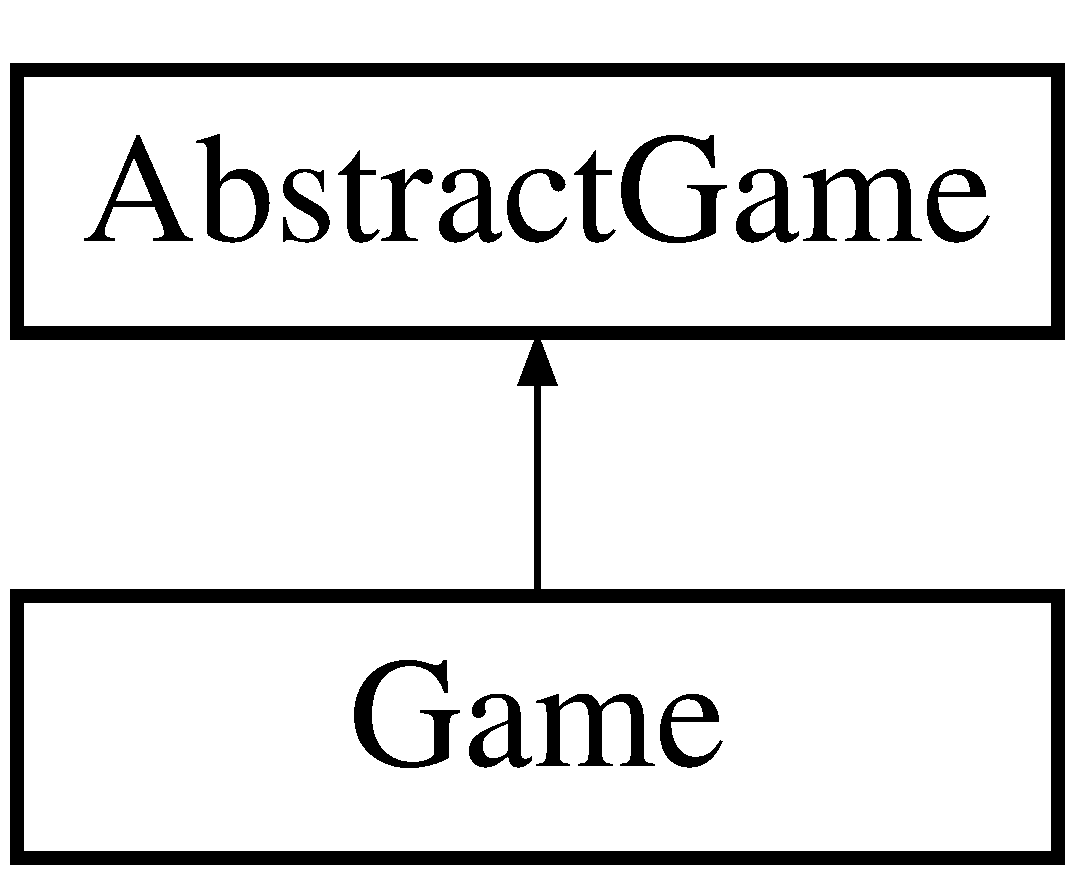
\includegraphics[height=2.000000cm]{class_game}
\end{center}
\end{figure}
\subsection*{Public Member Functions}
\begin{DoxyCompactItemize}
\item 
void \mbox{\hyperlink{class_game_a91946f348c9334abd083dfebfecdd31d}{on\+Init}} ()
\begin{DoxyCompactList}\small\item\em Prepare the game. \end{DoxyCompactList}\item 
void \mbox{\hyperlink{class_game_a0e1dd146112c54290e11d3e5f0a36fdd}{switch\+Screen}} (int screen\+Index)
\begin{DoxyCompactList}\small\item\em Switch the current screen to the screen with the given index \end{DoxyCompactList}\item 
\mbox{\Hypertarget{class_game_a0fa2c7df592f68efaecf267f48b9041c}\label{class_game_a0fa2c7df592f68efaecf267f48b9041c}} 
{\bfseries Abstract\+Game} ()
\end{DoxyCompactItemize}
\subsection*{Additional Inherited Members}


\subsection{Member Function Documentation}
\mbox{\Hypertarget{class_game_a91946f348c9334abd083dfebfecdd31d}\label{class_game_a91946f348c9334abd083dfebfecdd31d}} 
\index{Game@{Game}!on\+Init@{on\+Init}}
\index{on\+Init@{on\+Init}!Game@{Game}}
\subsubsection{\texorpdfstring{on\+Init()}{onInit()}}
{\footnotesize\ttfamily void Game\+::on\+Init (\begin{DoxyParamCaption}{ }\end{DoxyParamCaption})\hspace{0.3cm}{\ttfamily [virtual]}}



Prepare the game. 



Implements \mbox{\hyperlink{class_abstract_game_ae0bd76d926812f81e5e637ade3b1015f}{Abstract\+Game}}.

\mbox{\Hypertarget{class_game_a0e1dd146112c54290e11d3e5f0a36fdd}\label{class_game_a0e1dd146112c54290e11d3e5f0a36fdd}} 
\index{Game@{Game}!switch\+Screen@{switch\+Screen}}
\index{switch\+Screen@{switch\+Screen}!Game@{Game}}
\subsubsection{\texorpdfstring{switch\+Screen()}{switchScreen()}}
{\footnotesize\ttfamily void Game\+::switch\+Screen (\begin{DoxyParamCaption}\item[{int}]{screen\+Index }\end{DoxyParamCaption})\hspace{0.3cm}{\ttfamily [virtual]}}



Switch the current screen to the screen with the given index 


\begin{DoxyParams}{Parameters}
{\em screen\+Index} & The index of the screen we want to display\\
\hline
\end{DoxyParams}


Implements \mbox{\hyperlink{class_abstract_game_afd50e09c9b23aff40c752990947f07ce}{Abstract\+Game}}.



The documentation for this class was generated from the following files\+:\begin{DoxyCompactItemize}
\item 
Game.\+h\item 
Game.\+cpp\end{DoxyCompactItemize}

\hypertarget{class_game_object}{}\section{Game\+Object Class Reference}
\label{class_game_object}\index{Game\+Object@{Game\+Object}}
\subsection*{Public Member Functions}
\begin{DoxyCompactItemize}
\item 
\mbox{\Hypertarget{class_game_object_a8facf0ff97735803de908096859da1f9}\label{class_game_object_a8facf0ff97735803de908096859da1f9}} 
void {\bfseries add\+Extension} (shared\+\_\+ptr$<$ \mbox{\hyperlink{class_abstract_game_object_extension}{Abstract\+Game\+Object\+Extension}} $>$ extension)
\item 
\mbox{\Hypertarget{class_game_object_a611a94761cac7503507c88415d7085f3}\label{class_game_object_a611a94761cac7503507c88415d7085f3}} 
bool {\bfseries has\+Extension} (const std\+::type\+\_\+info \&type)
\item 
\mbox{\Hypertarget{class_game_object_a30f1fa65c3c058952b30ed8a08176d3c}\label{class_game_object_a30f1fa65c3c058952b30ed8a08176d3c}} 
shared\+\_\+ptr$<$ \mbox{\hyperlink{class_abstract_game_object_extension}{Abstract\+Game\+Object\+Extension}} $>$ {\bfseries get\+Extension} (const std\+::type\+\_\+info \&type)
\end{DoxyCompactItemize}
\subsection*{Public Attributes}
\begin{DoxyCompactItemize}
\item 
\mbox{\Hypertarget{class_game_object_a1171f2f6a12999c18dae12e027fbb7f3}\label{class_game_object_a1171f2f6a12999c18dae12e027fbb7f3}} 
\mbox{\hyperlink{class_physical_body}{Physical\+Body}} {\bfseries physical\+Body}
\item 
\mbox{\Hypertarget{class_game_object_abdf165736d0533f32dadca6e0e46b809}\label{class_game_object_abdf165736d0533f32dadca6e0e46b809}} 
std\+::string {\bfseries texture\+Path}
\end{DoxyCompactItemize}


The documentation for this class was generated from the following files\+:\begin{DoxyCompactItemize}
\item 
Game\+Object.\+h\item 
Game\+Object.\+cpp\end{DoxyCompactItemize}

\hypertarget{class_game_object_builder}{}\section{Game\+Object\+Builder Class Reference}
\label{class_game_object_builder}\index{Game\+Object\+Builder@{Game\+Object\+Builder}}
\subsection*{Public Member Functions}
\begin{DoxyCompactItemize}
\item 
\mbox{\Hypertarget{class_game_object_builder_aa6b134262f25c9210696ecc0be4d64b6}\label{class_game_object_builder_aa6b134262f25c9210696ecc0be4d64b6}} 
void {\bfseries build\+Game\+Object} ()
\item 
\mbox{\Hypertarget{class_game_object_builder_a86adfd2a3ac5d8fb98e9ab78caabbb87}\label{class_game_object_builder_a86adfd2a3ac5d8fb98e9ab78caabbb87}} 
void {\bfseries add\+Extension} (std\+::vector$<$ string $>$ extensions)
\item 
\mbox{\Hypertarget{class_game_object_builder_a7b8c868cad563c4afdf4ede8461438b6}\label{class_game_object_builder_a7b8c868cad563c4afdf4ede8461438b6}} 
shared\+\_\+ptr$<$ \mbox{\hyperlink{class_game_object}{Game\+Object}} $>$ {\bfseries get\+Result} ()
\end{DoxyCompactItemize}
\subsection*{Protected Attributes}
\begin{DoxyCompactItemize}
\item 
\mbox{\Hypertarget{class_game_object_builder_ac77339c64c7851f4134184298bcaf13d}\label{class_game_object_builder_ac77339c64c7851f4134184298bcaf13d}} 
std\+::shared\+\_\+ptr$<$ \mbox{\hyperlink{class_game_object}{Game\+Object}} $>$ {\bfseries \+\_\+game\+Object}
\end{DoxyCompactItemize}


The documentation for this class was generated from the following files\+:\begin{DoxyCompactItemize}
\item 
Game\+Object\+Builder.\+h\item 
Game\+Object\+Builder.\+cpp\end{DoxyCompactItemize}

\hypertarget{class_game_object_extension_factory}{}\section{Game\+Object\+Extension\+Factory Class Reference}
\label{class_game_object_extension_factory}\index{Game\+Object\+Extension\+Factory@{Game\+Object\+Extension\+Factory}}
\subsection*{Public Member Functions}
\begin{DoxyCompactItemize}
\item 
\mbox{\Hypertarget{class_game_object_extension_factory_ab9c2ed400c2ff14bb6fcb1e7bf7331e5}\label{class_game_object_extension_factory_ab9c2ed400c2ff14bb6fcb1e7bf7331e5}} 
void {\bfseries register\+Extension} (const string \&extension\+Name, Create\+Extension\+Fn pfn\+Create)
\item 
\mbox{\Hypertarget{class_game_object_extension_factory_af55575f9463d72d29493247e194d85b8}\label{class_game_object_extension_factory_af55575f9463d72d29493247e194d85b8}} 
\mbox{\hyperlink{class_abstract_game_object_extension}{Abstract\+Game\+Object\+Extension}} $\ast$ {\bfseries create\+Extension} (const string \&extension\+Name)
\end{DoxyCompactItemize}
\subsection*{Static Public Member Functions}
\begin{DoxyCompactItemize}
\item 
\mbox{\Hypertarget{class_game_object_extension_factory_a986654c9c23115ed7f8a5c0e43571b54}\label{class_game_object_extension_factory_a986654c9c23115ed7f8a5c0e43571b54}} 
static \mbox{\hyperlink{class_game_object_extension_factory}{Game\+Object\+Extension\+Factory}} $\ast$ {\bfseries get} ()
\end{DoxyCompactItemize}


The documentation for this class was generated from the following files\+:\begin{DoxyCompactItemize}
\item 
Game\+Object\+Extension\+Factory.\+h\item 
Game\+Object\+Extension\+Factory.\+cpp\end{DoxyCompactItemize}

\hypertarget{class_game_object_facade}{}\section{Game\+Object\+Facade Class Reference}
\label{class_game_object_facade}\index{Game\+Object\+Facade@{Game\+Object\+Facade}}


The documentation for this class was generated from the following file\+:\begin{DoxyCompactItemize}
\item 
Game\+Object\+Facade.\+h\end{DoxyCompactItemize}

\hypertarget{class_game_screen}{}\section{Game\+Screen Class Reference}
\label{class_game_screen}\index{Game\+Screen@{Game\+Screen}}
Inheritance diagram for Game\+Screen\+:\begin{figure}[H]
\begin{center}
\leavevmode
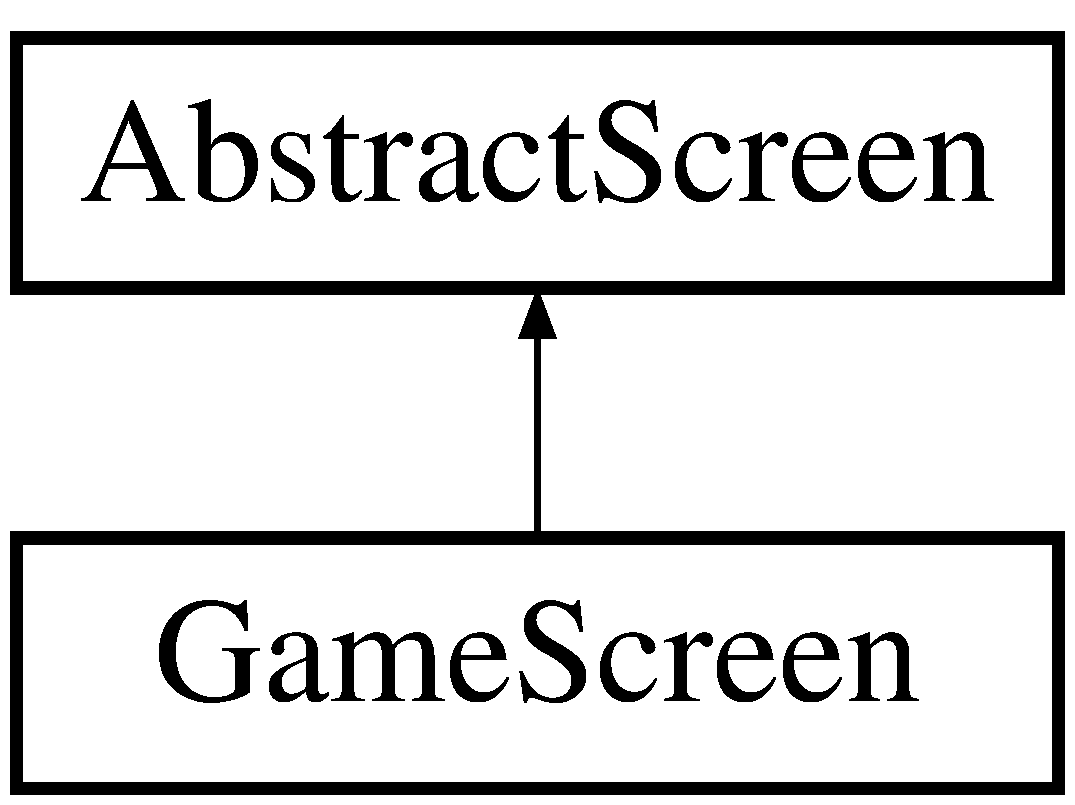
\includegraphics[height=2.000000cm]{class_game_screen}
\end{center}
\end{figure}
\subsection*{Public Member Functions}
\begin{DoxyCompactItemize}
\item 
void \mbox{\hyperlink{class_game_screen_a2748a44cf5e9ebe46f4e2e603bbfbae3}{on\+Init}} ()
\begin{DoxyCompactList}\small\item\em Called one time to create all objects. \end{DoxyCompactList}\item 
void \mbox{\hyperlink{class_game_screen_a0e2549c9c0198f925df16203998bb53b}{on\+Tick}} ()
\begin{DoxyCompactList}\small\item\em Called every tick to update properties. \end{DoxyCompactList}\item 
void \mbox{\hyperlink{class_game_screen_a1dfaea8cc8d0edb3bd2711d20e97ebeb}{on\+Screen\+Showed}} ()
\begin{DoxyCompactList}\small\item\em Called when the user switches to this screen. \end{DoxyCompactList}\item 
void \mbox{\hyperlink{class_game_screen_ae0cb9f2e2ca4016debdffa7f778f5627}{handle\+Keyboard\+Input}} (S\+D\+L\+\_\+\+Keyboard\+Event e)
\begin{DoxyCompactList}\small\item\em Called when the user uses their keyboard. \end{DoxyCompactList}\item 
void \mbox{\hyperlink{class_game_screen_af2fbc9a94d5b522870a9bfceea0f1da5}{handle\+Mouse\+Motion\+Input}} (S\+D\+L\+\_\+\+Mouse\+Motion\+Event e)
\begin{DoxyCompactList}\small\item\em Called when the user moves their mouse. \end{DoxyCompactList}\item 
void \mbox{\hyperlink{class_game_screen_abe56a9ed6eaac0df7459f681265e0dd2}{handle\+Mouse\+Click\+Input}} (S\+D\+L\+\_\+\+Mouse\+Button\+Event e)
\begin{DoxyCompactList}\small\item\em Called when the user click their mouse. \end{DoxyCompactList}\item 
\mbox{\Hypertarget{class_game_screen_a9c46f578b910897d268ce46b5057bf50}\label{class_game_screen_a9c46f578b910897d268ce46b5057bf50}} 
{\bfseries Abstract\+Screen} ()
\end{DoxyCompactItemize}
\subsection*{Additional Inherited Members}


\subsection{Member Function Documentation}
\mbox{\Hypertarget{class_game_screen_ae0cb9f2e2ca4016debdffa7f778f5627}\label{class_game_screen_ae0cb9f2e2ca4016debdffa7f778f5627}} 
\index{Game\+Screen@{Game\+Screen}!handle\+Keyboard\+Input@{handle\+Keyboard\+Input}}
\index{handle\+Keyboard\+Input@{handle\+Keyboard\+Input}!Game\+Screen@{Game\+Screen}}
\subsubsection{\texorpdfstring{handle\+Keyboard\+Input()}{handleKeyboardInput()}}
{\footnotesize\ttfamily void Game\+Screen\+::handle\+Keyboard\+Input (\begin{DoxyParamCaption}\item[{S\+D\+L\+\_\+\+Keyboard\+Event}]{e }\end{DoxyParamCaption})\hspace{0.3cm}{\ttfamily [virtual]}}



Called when the user uses their keyboard. 


\begin{DoxyParams}{Parameters}
{\em e} & The keyboard event.\\
\hline
\end{DoxyParams}


Implements \mbox{\hyperlink{class_abstract_screen_ad618b78e55faf59bab580e920461b790}{Abstract\+Screen}}.

\mbox{\Hypertarget{class_game_screen_abe56a9ed6eaac0df7459f681265e0dd2}\label{class_game_screen_abe56a9ed6eaac0df7459f681265e0dd2}} 
\index{Game\+Screen@{Game\+Screen}!handle\+Mouse\+Click\+Input@{handle\+Mouse\+Click\+Input}}
\index{handle\+Mouse\+Click\+Input@{handle\+Mouse\+Click\+Input}!Game\+Screen@{Game\+Screen}}
\subsubsection{\texorpdfstring{handle\+Mouse\+Click\+Input()}{handleMouseClickInput()}}
{\footnotesize\ttfamily void Game\+Screen\+::handle\+Mouse\+Click\+Input (\begin{DoxyParamCaption}\item[{S\+D\+L\+\_\+\+Mouse\+Button\+Event}]{e }\end{DoxyParamCaption})\hspace{0.3cm}{\ttfamily [virtual]}}



Called when the user click their mouse. 


\begin{DoxyParams}{Parameters}
{\em e} & The mouse click event.\\
\hline
\end{DoxyParams}


Implements \mbox{\hyperlink{class_abstract_screen_a9f9631ff1a9078b96bcf31e062f7379e}{Abstract\+Screen}}.

\mbox{\Hypertarget{class_game_screen_af2fbc9a94d5b522870a9bfceea0f1da5}\label{class_game_screen_af2fbc9a94d5b522870a9bfceea0f1da5}} 
\index{Game\+Screen@{Game\+Screen}!handle\+Mouse\+Motion\+Input@{handle\+Mouse\+Motion\+Input}}
\index{handle\+Mouse\+Motion\+Input@{handle\+Mouse\+Motion\+Input}!Game\+Screen@{Game\+Screen}}
\subsubsection{\texorpdfstring{handle\+Mouse\+Motion\+Input()}{handleMouseMotionInput()}}
{\footnotesize\ttfamily void Game\+Screen\+::handle\+Mouse\+Motion\+Input (\begin{DoxyParamCaption}\item[{S\+D\+L\+\_\+\+Mouse\+Motion\+Event}]{e }\end{DoxyParamCaption})\hspace{0.3cm}{\ttfamily [virtual]}}



Called when the user moves their mouse. 


\begin{DoxyParams}{Parameters}
{\em e} & The mouse mouse event.\\
\hline
\end{DoxyParams}


Implements \mbox{\hyperlink{class_abstract_screen_ab05039a94ee494811800187787636d2b}{Abstract\+Screen}}.

\mbox{\Hypertarget{class_game_screen_a2748a44cf5e9ebe46f4e2e603bbfbae3}\label{class_game_screen_a2748a44cf5e9ebe46f4e2e603bbfbae3}} 
\index{Game\+Screen@{Game\+Screen}!on\+Init@{on\+Init}}
\index{on\+Init@{on\+Init}!Game\+Screen@{Game\+Screen}}
\subsubsection{\texorpdfstring{on\+Init()}{onInit()}}
{\footnotesize\ttfamily void Game\+Screen\+::on\+Init (\begin{DoxyParamCaption}{ }\end{DoxyParamCaption})\hspace{0.3cm}{\ttfamily [virtual]}}



Called one time to create all objects. 



Implements \mbox{\hyperlink{class_abstract_screen_a7ab389bd33f4824d3d353b5a9e1616de}{Abstract\+Screen}}.

\mbox{\Hypertarget{class_game_screen_a1dfaea8cc8d0edb3bd2711d20e97ebeb}\label{class_game_screen_a1dfaea8cc8d0edb3bd2711d20e97ebeb}} 
\index{Game\+Screen@{Game\+Screen}!on\+Screen\+Showed@{on\+Screen\+Showed}}
\index{on\+Screen\+Showed@{on\+Screen\+Showed}!Game\+Screen@{Game\+Screen}}
\subsubsection{\texorpdfstring{on\+Screen\+Showed()}{onScreenShowed()}}
{\footnotesize\ttfamily void Game\+Screen\+::on\+Screen\+Showed (\begin{DoxyParamCaption}{ }\end{DoxyParamCaption})\hspace{0.3cm}{\ttfamily [virtual]}}



Called when the user switches to this screen. 



Implements \mbox{\hyperlink{class_abstract_screen_a219687a34e6aed15a9eaf0d4414d1783}{Abstract\+Screen}}.

\mbox{\Hypertarget{class_game_screen_a0e2549c9c0198f925df16203998bb53b}\label{class_game_screen_a0e2549c9c0198f925df16203998bb53b}} 
\index{Game\+Screen@{Game\+Screen}!on\+Tick@{on\+Tick}}
\index{on\+Tick@{on\+Tick}!Game\+Screen@{Game\+Screen}}
\subsubsection{\texorpdfstring{on\+Tick()}{onTick()}}
{\footnotesize\ttfamily void Game\+Screen\+::on\+Tick (\begin{DoxyParamCaption}{ }\end{DoxyParamCaption})\hspace{0.3cm}{\ttfamily [virtual]}}



Called every tick to update properties. 



Implements \mbox{\hyperlink{class_abstract_screen_a3861213630fd23d4a3ff392191614ec2}{Abstract\+Screen}}.



The documentation for this class was generated from the following files\+:\begin{DoxyCompactItemize}
\item 
Game\+Screen.\+h\item 
Game\+Screen.\+cpp\end{DoxyCompactItemize}

\hypertarget{class_health_extension}{}\section{Health\+Extension Class Reference}
\label{class_health_extension}\index{Health\+Extension@{Health\+Extension}}
Inheritance diagram for Health\+Extension\+:\begin{figure}[H]
\begin{center}
\leavevmode
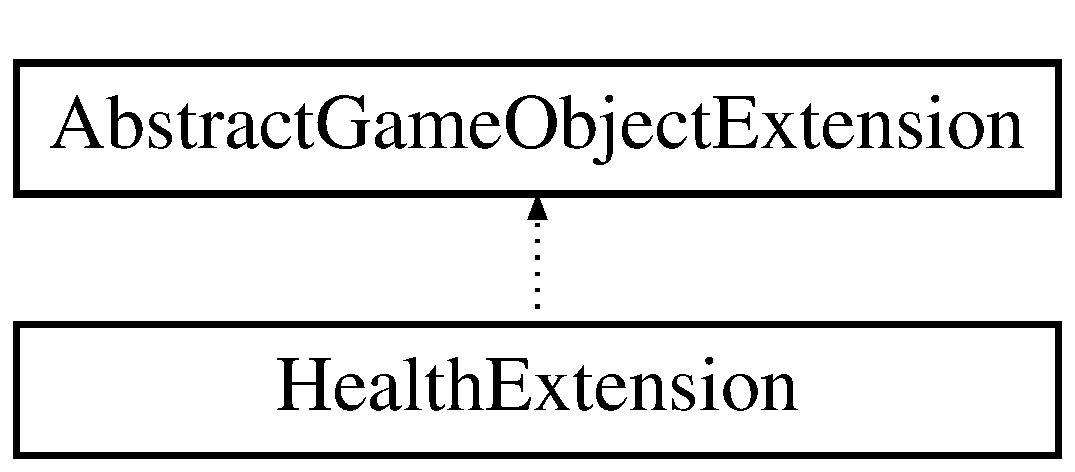
\includegraphics[height=2.000000cm]{class_health_extension}
\end{center}
\end{figure}
\subsection*{Static Public Member Functions}
\begin{DoxyCompactItemize}
\item 
\mbox{\Hypertarget{class_health_extension_a367da40b097a96a692e38ab3a22827b2}\label{class_health_extension_a367da40b097a96a692e38ab3a22827b2}} 
static \mbox{\hyperlink{class_abstract_game_object_extension}{Abstract\+Game\+Object\+Extension}} $\ast$\+\_\+\+\_\+stdcall {\bfseries create} ()
\end{DoxyCompactItemize}


The documentation for this class was generated from the following file\+:\begin{DoxyCompactItemize}
\item 
Health\+Extension.\+h\end{DoxyCompactItemize}

\hypertarget{class_image_ui_element}{}\section{Image\+Ui\+Element Class Reference}
\label{class_image_ui_element}\index{Image\+Ui\+Element@{Image\+Ui\+Element}}
Inheritance diagram for Image\+Ui\+Element\+:\begin{figure}[H]
\begin{center}
\leavevmode
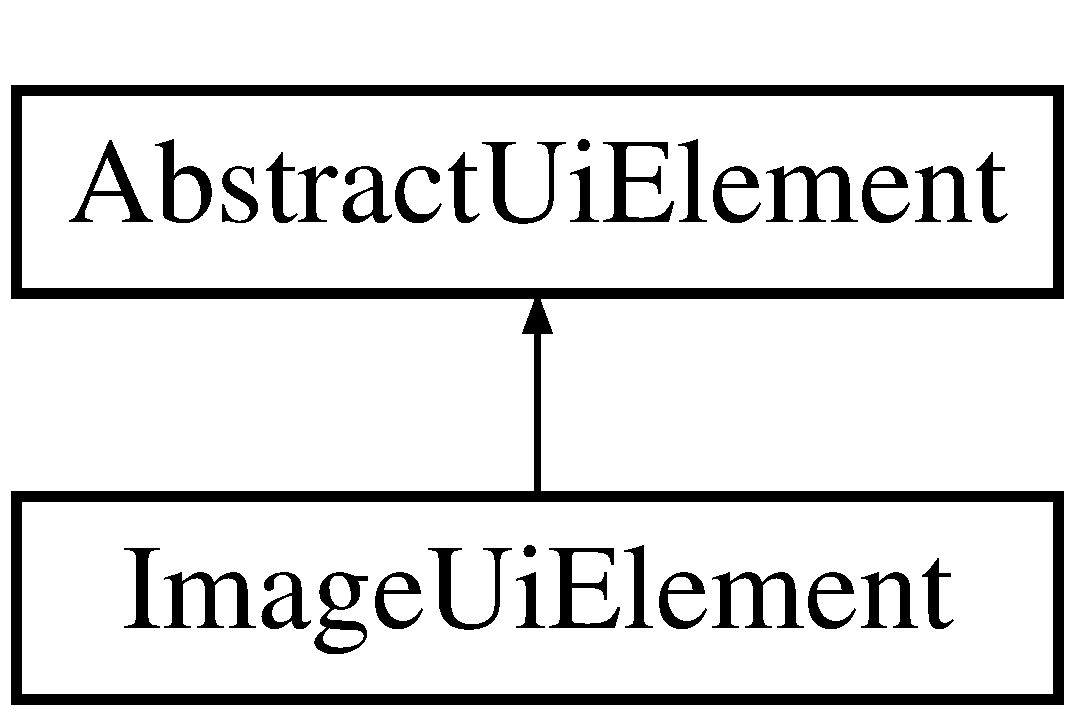
\includegraphics[height=2.000000cm]{class_image_ui_element}
\end{center}
\end{figure}
\subsection*{Public Member Functions}
\begin{DoxyCompactItemize}
\item 
\mbox{\Hypertarget{class_image_ui_element_aaa4540956ec81cef649694d1d45b28dd}\label{class_image_ui_element_aaa4540956ec81cef649694d1d45b28dd}} 
{\bfseries Image\+Ui\+Element} (std\+::string file\+Path, S\+D\+L\+\_\+\+Rect rect)
\item 
void \mbox{\hyperlink{class_image_ui_element_a422fc1d3b4c1451f656e7470e575577b}{render}} (S\+D\+L\+\_\+\+Renderer $\ast$renderer)
\begin{DoxyCompactList}\small\item\em Render the element on the screen. \end{DoxyCompactList}\item 
void \mbox{\hyperlink{class_image_ui_element_ab3c388de0807d86016a2ff43fd6d337e}{on\+Click}} ()
\begin{DoxyCompactList}\small\item\em The function executed when the element is clicked on. \end{DoxyCompactList}\item 
bool \mbox{\hyperlink{class_image_ui_element_a6d0f66cf68c5f035f5a9bfeaba3028f4}{is\+In\+Bound}} (int mouseX, int mouseY)
\begin{DoxyCompactList}\small\item\em Checks if the mouse is within the bounds of the element. \end{DoxyCompactList}\end{DoxyCompactItemize}
\subsection*{Additional Inherited Members}


\subsection{Member Function Documentation}
\mbox{\Hypertarget{class_image_ui_element_a6d0f66cf68c5f035f5a9bfeaba3028f4}\label{class_image_ui_element_a6d0f66cf68c5f035f5a9bfeaba3028f4}} 
\index{Image\+Ui\+Element@{Image\+Ui\+Element}!is\+In\+Bound@{is\+In\+Bound}}
\index{is\+In\+Bound@{is\+In\+Bound}!Image\+Ui\+Element@{Image\+Ui\+Element}}
\subsubsection{\texorpdfstring{is\+In\+Bound()}{isInBound()}}
{\footnotesize\ttfamily bool Image\+Ui\+Element\+::is\+In\+Bound (\begin{DoxyParamCaption}\item[{int}]{mouseX,  }\item[{int}]{mouseY }\end{DoxyParamCaption})\hspace{0.3cm}{\ttfamily [virtual]}}



Checks if the mouse is within the bounds of the element. 


\begin{DoxyParams}{Parameters}
{\em mouseX} & X coordinate of the mouse\\
\hline
{\em mouseY} & Y coordinate of the mouse\\
\hline
\end{DoxyParams}
\begin{DoxyReturn}{Returns}

\end{DoxyReturn}


Implements \mbox{\hyperlink{class_abstract_ui_element_ad2c415461cd7e8c1ee50b1105eb84685}{Abstract\+Ui\+Element}}.

\mbox{\Hypertarget{class_image_ui_element_ab3c388de0807d86016a2ff43fd6d337e}\label{class_image_ui_element_ab3c388de0807d86016a2ff43fd6d337e}} 
\index{Image\+Ui\+Element@{Image\+Ui\+Element}!on\+Click@{on\+Click}}
\index{on\+Click@{on\+Click}!Image\+Ui\+Element@{Image\+Ui\+Element}}
\subsubsection{\texorpdfstring{on\+Click()}{onClick()}}
{\footnotesize\ttfamily void Image\+Ui\+Element\+::on\+Click (\begin{DoxyParamCaption}{ }\end{DoxyParamCaption})\hspace{0.3cm}{\ttfamily [virtual]}}



The function executed when the element is clicked on. 



Implements \mbox{\hyperlink{class_abstract_ui_element_a42296c15c9e70b6ac7fda0b1862612af}{Abstract\+Ui\+Element}}.

\mbox{\Hypertarget{class_image_ui_element_a422fc1d3b4c1451f656e7470e575577b}\label{class_image_ui_element_a422fc1d3b4c1451f656e7470e575577b}} 
\index{Image\+Ui\+Element@{Image\+Ui\+Element}!render@{render}}
\index{render@{render}!Image\+Ui\+Element@{Image\+Ui\+Element}}
\subsubsection{\texorpdfstring{render()}{render()}}
{\footnotesize\ttfamily void Image\+Ui\+Element\+::render (\begin{DoxyParamCaption}\item[{S\+D\+L\+\_\+\+Renderer $\ast$}]{renderer }\end{DoxyParamCaption})\hspace{0.3cm}{\ttfamily [virtual]}}



Render the element on the screen. 


\begin{DoxyParams}{Parameters}
{\em renderer} & The renderer\\
\hline
\end{DoxyParams}


Implements \mbox{\hyperlink{class_abstract_ui_element_afacedc89a5805d95d3bdcf20619b1c06}{Abstract\+Ui\+Element}}.



The documentation for this class was generated from the following files\+:\begin{DoxyCompactItemize}
\item 
Image\+Ui\+Element.\+h\item 
Image\+Ui\+Element.\+cpp\end{DoxyCompactItemize}

\hypertarget{classmain}{}\section{main Class Reference}
\label{classmain}\index{main@{main}}


The documentation for this class was generated from the following file\+:\begin{DoxyCompactItemize}
\item 
main.\+h\end{DoxyCompactItemize}

\hypertarget{class_manifold}{}\section{Manifold Class Reference}
\label{class_manifold}\index{Manifold@{Manifold}}
\subsection*{Public Member Functions}
\begin{DoxyCompactItemize}
\item 
\mbox{\Hypertarget{class_manifold_a7a30f055ee040a7ac00284fb08b3c347}\label{class_manifold_a7a30f055ee040a7ac00284fb08b3c347}} 
{\bfseries Manifold} (\mbox{\hyperlink{class_physical_body}{Physical\+Body}} bodyA, \mbox{\hyperlink{class_physical_body}{Physical\+Body}} bodyB)
\item 
\mbox{\Hypertarget{class_manifold_a27080a445e565949f9e15b8fea69f6c0}\label{class_manifold_a27080a445e565949f9e15b8fea69f6c0}} 
void {\bfseries Apply\+Impulse} ()
\item 
\mbox{\Hypertarget{class_manifold_a9d3187192136eac849265f7d386f617e}\label{class_manifold_a9d3187192136eac849265f7d386f617e}} 
void {\bfseries Positional\+Correction} ()
\item 
\mbox{\Hypertarget{class_manifold_a09f7dd163c965856905247bb15a1ee99}\label{class_manifold_a09f7dd163c965856905247bb15a1ee99}} 
bool {\bfseries A\+A\+B\+Bvs\+A\+A\+BB} ()
\end{DoxyCompactItemize}
\subsection*{Public Attributes}
\begin{DoxyCompactItemize}
\item 
\mbox{\Hypertarget{class_manifold_a058391b5a2e745467c3da071408e631f}\label{class_manifold_a058391b5a2e745467c3da071408e631f}} 
real {\bfseries penetration}
\item 
\mbox{\Hypertarget{class_manifold_a08837c3bbf15c2dd1cb51d984698ab46}\label{class_manifold_a08837c3bbf15c2dd1cb51d984698ab46}} 
\mbox{\hyperlink{struct_vec2}{Vec2}} {\bfseries normal}
\item 
\mbox{\Hypertarget{class_manifold_a0f3863f327800fdf7b5bfab8db88a6dc}\label{class_manifold_a0f3863f327800fdf7b5bfab8db88a6dc}} 
\mbox{\hyperlink{struct_vec2}{Vec2}} {\bfseries contacts} \mbox{[}2\mbox{]}
\item 
\mbox{\Hypertarget{class_manifold_af98bbea7321829c3547ec8365f40f068}\label{class_manifold_af98bbea7321829c3547ec8365f40f068}} 
uint32 {\bfseries contact\+\_\+count}
\item 
\mbox{\Hypertarget{class_manifold_a7eb7fecdb3dbac0ad387ac9893f91180}\label{class_manifold_a7eb7fecdb3dbac0ad387ac9893f91180}} 
real {\bfseries e}
\item 
\mbox{\Hypertarget{class_manifold_ac8b98d3211f99d8997b96a5c95ba80f1}\label{class_manifold_ac8b98d3211f99d8997b96a5c95ba80f1}} 
real {\bfseries df}
\item 
\mbox{\Hypertarget{class_manifold_ad7ccd59e59bb27f236ea6a2d05a765e4}\label{class_manifold_ad7ccd59e59bb27f236ea6a2d05a765e4}} 
real {\bfseries sf}
\end{DoxyCompactItemize}


The documentation for this class was generated from the following files\+:\begin{DoxyCompactItemize}
\item 
Manifold.\+h\item 
Manifold.\+cpp\end{DoxyCompactItemize}

\hypertarget{class_mass_data}{}\section{Mass\+Data Class Reference}
\label{class_mass_data}\index{Mass\+Data@{Mass\+Data}}


The documentation for this class was generated from the following file\+:\begin{DoxyCompactItemize}
\item 
Mass\+Data.\+h\end{DoxyCompactItemize}

\hypertarget{class_material}{}\section{Material Class Reference}
\label{class_material}\index{Material@{Material}}


The documentation for this class was generated from the following file\+:\begin{DoxyCompactItemize}
\item 
Material.\+h\end{DoxyCompactItemize}

\hypertarget{class_move_extension}{}\section{Move\+Extension Class Reference}
\label{class_move_extension}\index{Move\+Extension@{Move\+Extension}}
Inheritance diagram for Move\+Extension\+:\begin{figure}[H]
\begin{center}
\leavevmode
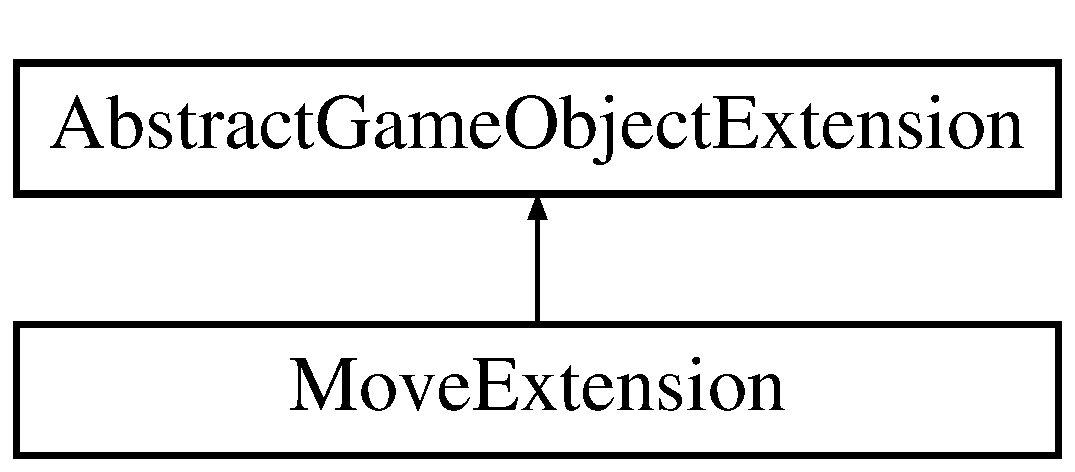
\includegraphics[height=2.000000cm]{class_move_extension}
\end{center}
\end{figure}
\subsection*{Public Member Functions}
\begin{DoxyCompactItemize}
\item 
\mbox{\Hypertarget{class_move_extension_a8970d97c5d87073eb2255bb1b29fd8fc}\label{class_move_extension_a8970d97c5d87073eb2255bb1b29fd8fc}} 
void {\bfseries move} ()
\end{DoxyCompactItemize}
\subsection*{Static Public Member Functions}
\begin{DoxyCompactItemize}
\item 
\mbox{\Hypertarget{class_move_extension_a45554f4b247dd795a9e8e71614ab677a}\label{class_move_extension_a45554f4b247dd795a9e8e71614ab677a}} 
static \mbox{\hyperlink{class_abstract_game_object_extension}{Abstract\+Game\+Object\+Extension}} $\ast$\+\_\+\+\_\+stdcall {\bfseries create} ()
\end{DoxyCompactItemize}
\subsection*{Additional Inherited Members}


The documentation for this class was generated from the following files\+:\begin{DoxyCompactItemize}
\item 
Move\+Extension.\+h\item 
Move\+Extension.\+cpp\end{DoxyCompactItemize}

\hypertarget{class_pause_screen}{}\section{Pause\+Screen Class Reference}
\label{class_pause_screen}\index{Pause\+Screen@{Pause\+Screen}}
Inheritance diagram for Pause\+Screen\+:\begin{figure}[H]
\begin{center}
\leavevmode
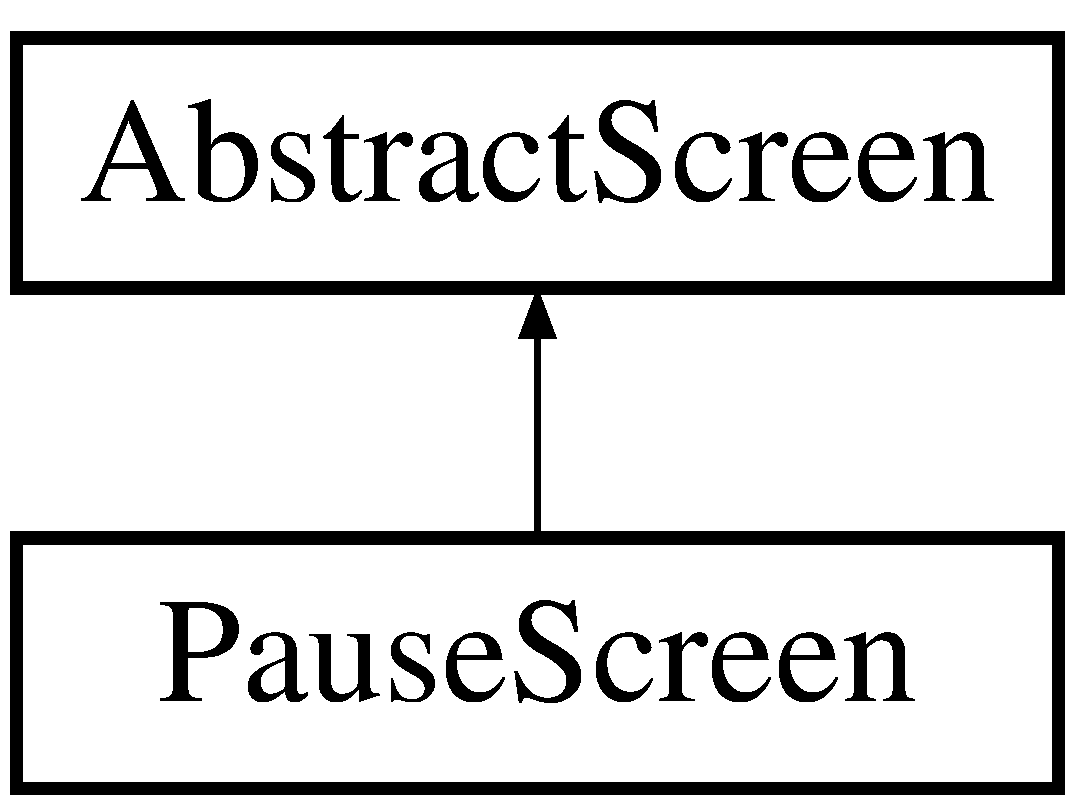
\includegraphics[height=2.000000cm]{class_pause_screen}
\end{center}
\end{figure}
\subsection*{Public Member Functions}
\begin{DoxyCompactItemize}
\item 
void \mbox{\hyperlink{class_pause_screen_ae8196adf49b2e7439677a5360a8d43d4}{on\+Init}} ()
\begin{DoxyCompactList}\small\item\em Called one time to create all objects. \end{DoxyCompactList}\item 
void \mbox{\hyperlink{class_pause_screen_a89ef5189bdc9acfae5eedbff2cf4b458}{on\+Tick}} ()
\begin{DoxyCompactList}\small\item\em Called every tick to update properties. \end{DoxyCompactList}\item 
void \mbox{\hyperlink{class_pause_screen_a2eb2b032a3c3e833beb505c2df12396b}{on\+Screen\+Showed}} ()
\begin{DoxyCompactList}\small\item\em Called when the user switches to this screen. \end{DoxyCompactList}\item 
void \mbox{\hyperlink{class_pause_screen_a94112a789c88bdf68809b09ec86049c8}{handle\+Keyboard\+Input}} (S\+D\+L\+\_\+\+Keyboard\+Event e)
\begin{DoxyCompactList}\small\item\em Called when the user uses their keyboard. \end{DoxyCompactList}\item 
void \mbox{\hyperlink{class_pause_screen_a19ce9a528ab648afb81a2251810afcfa}{handle\+Mouse\+Motion\+Input}} (S\+D\+L\+\_\+\+Mouse\+Motion\+Event e)
\begin{DoxyCompactList}\small\item\em Called when the user moves their mouse. \end{DoxyCompactList}\item 
void \mbox{\hyperlink{class_pause_screen_a82ce01aa34df937a0f072d6210ac4386}{handle\+Mouse\+Click\+Input}} (S\+D\+L\+\_\+\+Mouse\+Button\+Event e)
\begin{DoxyCompactList}\small\item\em Called when the user click their mouse. \end{DoxyCompactList}\item 
\mbox{\Hypertarget{class_pause_screen_a9c46f578b910897d268ce46b5057bf50}\label{class_pause_screen_a9c46f578b910897d268ce46b5057bf50}} 
{\bfseries Abstract\+Screen} ()
\end{DoxyCompactItemize}
\subsection*{Additional Inherited Members}


\subsection{Member Function Documentation}
\mbox{\Hypertarget{class_pause_screen_a94112a789c88bdf68809b09ec86049c8}\label{class_pause_screen_a94112a789c88bdf68809b09ec86049c8}} 
\index{Pause\+Screen@{Pause\+Screen}!handle\+Keyboard\+Input@{handle\+Keyboard\+Input}}
\index{handle\+Keyboard\+Input@{handle\+Keyboard\+Input}!Pause\+Screen@{Pause\+Screen}}
\subsubsection{\texorpdfstring{handle\+Keyboard\+Input()}{handleKeyboardInput()}}
{\footnotesize\ttfamily void Pause\+Screen\+::handle\+Keyboard\+Input (\begin{DoxyParamCaption}\item[{S\+D\+L\+\_\+\+Keyboard\+Event}]{e }\end{DoxyParamCaption})\hspace{0.3cm}{\ttfamily [virtual]}}



Called when the user uses their keyboard. 


\begin{DoxyParams}{Parameters}
{\em e} & The keyboard event.\\
\hline
\end{DoxyParams}


Implements \mbox{\hyperlink{class_abstract_screen_ad618b78e55faf59bab580e920461b790}{Abstract\+Screen}}.

\mbox{\Hypertarget{class_pause_screen_a82ce01aa34df937a0f072d6210ac4386}\label{class_pause_screen_a82ce01aa34df937a0f072d6210ac4386}} 
\index{Pause\+Screen@{Pause\+Screen}!handle\+Mouse\+Click\+Input@{handle\+Mouse\+Click\+Input}}
\index{handle\+Mouse\+Click\+Input@{handle\+Mouse\+Click\+Input}!Pause\+Screen@{Pause\+Screen}}
\subsubsection{\texorpdfstring{handle\+Mouse\+Click\+Input()}{handleMouseClickInput()}}
{\footnotesize\ttfamily void Pause\+Screen\+::handle\+Mouse\+Click\+Input (\begin{DoxyParamCaption}\item[{S\+D\+L\+\_\+\+Mouse\+Button\+Event}]{e }\end{DoxyParamCaption})\hspace{0.3cm}{\ttfamily [virtual]}}



Called when the user click their mouse. 


\begin{DoxyParams}{Parameters}
{\em e} & The mouse click event.\\
\hline
\end{DoxyParams}


Implements \mbox{\hyperlink{class_abstract_screen_a9f9631ff1a9078b96bcf31e062f7379e}{Abstract\+Screen}}.

\mbox{\Hypertarget{class_pause_screen_a19ce9a528ab648afb81a2251810afcfa}\label{class_pause_screen_a19ce9a528ab648afb81a2251810afcfa}} 
\index{Pause\+Screen@{Pause\+Screen}!handle\+Mouse\+Motion\+Input@{handle\+Mouse\+Motion\+Input}}
\index{handle\+Mouse\+Motion\+Input@{handle\+Mouse\+Motion\+Input}!Pause\+Screen@{Pause\+Screen}}
\subsubsection{\texorpdfstring{handle\+Mouse\+Motion\+Input()}{handleMouseMotionInput()}}
{\footnotesize\ttfamily void Pause\+Screen\+::handle\+Mouse\+Motion\+Input (\begin{DoxyParamCaption}\item[{S\+D\+L\+\_\+\+Mouse\+Motion\+Event}]{e }\end{DoxyParamCaption})\hspace{0.3cm}{\ttfamily [virtual]}}



Called when the user moves their mouse. 


\begin{DoxyParams}{Parameters}
{\em e} & The mouse mouse event.\\
\hline
\end{DoxyParams}


Implements \mbox{\hyperlink{class_abstract_screen_ab05039a94ee494811800187787636d2b}{Abstract\+Screen}}.

\mbox{\Hypertarget{class_pause_screen_ae8196adf49b2e7439677a5360a8d43d4}\label{class_pause_screen_ae8196adf49b2e7439677a5360a8d43d4}} 
\index{Pause\+Screen@{Pause\+Screen}!on\+Init@{on\+Init}}
\index{on\+Init@{on\+Init}!Pause\+Screen@{Pause\+Screen}}
\subsubsection{\texorpdfstring{on\+Init()}{onInit()}}
{\footnotesize\ttfamily void Pause\+Screen\+::on\+Init (\begin{DoxyParamCaption}{ }\end{DoxyParamCaption})\hspace{0.3cm}{\ttfamily [virtual]}}



Called one time to create all objects. 



Implements \mbox{\hyperlink{class_abstract_screen_a7ab389bd33f4824d3d353b5a9e1616de}{Abstract\+Screen}}.

\mbox{\Hypertarget{class_pause_screen_a2eb2b032a3c3e833beb505c2df12396b}\label{class_pause_screen_a2eb2b032a3c3e833beb505c2df12396b}} 
\index{Pause\+Screen@{Pause\+Screen}!on\+Screen\+Showed@{on\+Screen\+Showed}}
\index{on\+Screen\+Showed@{on\+Screen\+Showed}!Pause\+Screen@{Pause\+Screen}}
\subsubsection{\texorpdfstring{on\+Screen\+Showed()}{onScreenShowed()}}
{\footnotesize\ttfamily void Pause\+Screen\+::on\+Screen\+Showed (\begin{DoxyParamCaption}{ }\end{DoxyParamCaption})\hspace{0.3cm}{\ttfamily [virtual]}}



Called when the user switches to this screen. 



Implements \mbox{\hyperlink{class_abstract_screen_a219687a34e6aed15a9eaf0d4414d1783}{Abstract\+Screen}}.

\mbox{\Hypertarget{class_pause_screen_a89ef5189bdc9acfae5eedbff2cf4b458}\label{class_pause_screen_a89ef5189bdc9acfae5eedbff2cf4b458}} 
\index{Pause\+Screen@{Pause\+Screen}!on\+Tick@{on\+Tick}}
\index{on\+Tick@{on\+Tick}!Pause\+Screen@{Pause\+Screen}}
\subsubsection{\texorpdfstring{on\+Tick()}{onTick()}}
{\footnotesize\ttfamily void Pause\+Screen\+::on\+Tick (\begin{DoxyParamCaption}{ }\end{DoxyParamCaption})\hspace{0.3cm}{\ttfamily [virtual]}}



Called every tick to update properties. 



Implements \mbox{\hyperlink{class_abstract_screen_a3861213630fd23d4a3ff392191614ec2}{Abstract\+Screen}}.



The documentation for this class was generated from the following files\+:\begin{DoxyCompactItemize}
\item 
Pause\+Screen.\+h\item 
Pause\+Screen.\+cpp\end{DoxyCompactItemize}

\hypertarget{class_physical_body}{}\section{Physical\+Body Class Reference}
\label{class_physical_body}\index{Physical\+Body@{Physical\+Body}}
\subsection*{Public Attributes}
\begin{DoxyCompactItemize}
\item 
\mbox{\Hypertarget{class_physical_body_a5c08e14cfcaa3474aa98d35c612a61b9}\label{class_physical_body_a5c08e14cfcaa3474aa98d35c612a61b9}} 
\mbox{\hyperlink{class_shape}{Shape}} {\bfseries shape}
\item 
\mbox{\Hypertarget{class_physical_body_aa4550abc8868d01384a54188a0ad8bd9}\label{class_physical_body_aa4550abc8868d01384a54188a0ad8bd9}} 
\mbox{\hyperlink{struct_body}{Body}} {\bfseries body}
\end{DoxyCompactItemize}


The documentation for this class was generated from the following file\+:\begin{DoxyCompactItemize}
\item 
Physical\+Body.\+h\end{DoxyCompactItemize}

\hypertarget{class_physics}{}\section{Physics Class Reference}
\label{class_physics}\index{Physics@{Physics}}


\mbox{\hyperlink{class_physics}{Physics}} Helper for \mbox{\hyperlink{class_game}{Game}} \mbox{\hyperlink{class_physics}{Physics}}  




{\ttfamily \#include $<$Physics.\+h$>$}

\subsection*{Public Member Functions}
\begin{DoxyCompactItemize}
\item 
void \mbox{\hyperlink{class_physics_a3baa430406c9017c1de92ed9c35dc9a2}{change\+Velocity}} (shared\+\_\+ptr$<$ \mbox{\hyperlink{class_game_object}{Game\+Object}} $>$ object, \mbox{\hyperlink{struct_vec2}{Vec2}} velocity)
\begin{DoxyCompactList}\small\item\em Change the velocity of a game object \end{DoxyCompactList}\item 
void \mbox{\hyperlink{class_physics_aef3b1d8a37d4eea381dfe48779188b38}{set\+Position}} (shared\+\_\+ptr$<$ \mbox{\hyperlink{class_game_object}{Game\+Object}} $>$ object, \mbox{\hyperlink{struct_vec2}{Vec2}} position)
\begin{DoxyCompactList}\small\item\em Set the position of a game object \end{DoxyCompactList}\item 
void \mbox{\hyperlink{class_physics_acd65e09cdd0dbb9648956c8d174bb621}{update\+Position}} (shared\+\_\+ptr$<$ \mbox{\hyperlink{class_game_object}{Game\+Object}} $>$ object)
\begin{DoxyCompactList}\small\item\em Update the position of a game object, applying all physics forces like gravity. \end{DoxyCompactList}\item 
void \mbox{\hyperlink{class_physics_a00639bda7da3c9e8c8b726de6104c64d}{add\+Gravity\+Force}} (shared\+\_\+ptr$<$ \mbox{\hyperlink{class_game_object}{Game\+Object}} $>$ object)
\begin{DoxyCompactList}\small\item\em Add gravity to a game object \end{DoxyCompactList}\end{DoxyCompactItemize}


\subsection{Detailed Description}
\mbox{\hyperlink{class_physics}{Physics}} Helper for \mbox{\hyperlink{class_game}{Game}} \mbox{\hyperlink{class_physics}{Physics}} 



\subsection{Member Function Documentation}
\mbox{\Hypertarget{class_physics_a00639bda7da3c9e8c8b726de6104c64d}\label{class_physics_a00639bda7da3c9e8c8b726de6104c64d}} 
\index{Physics@{Physics}!add\+Gravity\+Force@{add\+Gravity\+Force}}
\index{add\+Gravity\+Force@{add\+Gravity\+Force}!Physics@{Physics}}
\subsubsection{\texorpdfstring{add\+Gravity\+Force()}{addGravityForce()}}
{\footnotesize\ttfamily void Physics\+::add\+Gravity\+Force (\begin{DoxyParamCaption}\item[{shared\+\_\+ptr$<$ \mbox{\hyperlink{class_game_object}{Game\+Object}} $>$}]{object }\end{DoxyParamCaption})}



Add gravity to a game object 


\begin{DoxyParams}{Parameters}
{\em object} & The game object to get Gravity\\
\hline
\end{DoxyParams}
\mbox{\Hypertarget{class_physics_a3baa430406c9017c1de92ed9c35dc9a2}\label{class_physics_a3baa430406c9017c1de92ed9c35dc9a2}} 
\index{Physics@{Physics}!change\+Velocity@{change\+Velocity}}
\index{change\+Velocity@{change\+Velocity}!Physics@{Physics}}
\subsubsection{\texorpdfstring{change\+Velocity()}{changeVelocity()}}
{\footnotesize\ttfamily void Physics\+::change\+Velocity (\begin{DoxyParamCaption}\item[{shared\+\_\+ptr$<$ \mbox{\hyperlink{class_game_object}{Game\+Object}} $>$}]{object,  }\item[{\mbox{\hyperlink{struct_vec2}{Vec2}}}]{velocity }\end{DoxyParamCaption})}



Change the velocity of a game object 


\begin{DoxyParams}{Parameters}
{\em object} & The object to be changed\\
\hline
{\em velocity} & The new velocity\\
\hline
\end{DoxyParams}
\mbox{\Hypertarget{class_physics_aef3b1d8a37d4eea381dfe48779188b38}\label{class_physics_aef3b1d8a37d4eea381dfe48779188b38}} 
\index{Physics@{Physics}!set\+Position@{set\+Position}}
\index{set\+Position@{set\+Position}!Physics@{Physics}}
\subsubsection{\texorpdfstring{set\+Position()}{setPosition()}}
{\footnotesize\ttfamily void Physics\+::set\+Position (\begin{DoxyParamCaption}\item[{shared\+\_\+ptr$<$ \mbox{\hyperlink{class_game_object}{Game\+Object}} $>$}]{object,  }\item[{\mbox{\hyperlink{struct_vec2}{Vec2}}}]{position }\end{DoxyParamCaption})}



Set the position of a game object 


\begin{DoxyParams}{Parameters}
{\em object} & The object to be changed\\
\hline
{\em position} & The new position\\
\hline
\end{DoxyParams}
\mbox{\Hypertarget{class_physics_acd65e09cdd0dbb9648956c8d174bb621}\label{class_physics_acd65e09cdd0dbb9648956c8d174bb621}} 
\index{Physics@{Physics}!update\+Position@{update\+Position}}
\index{update\+Position@{update\+Position}!Physics@{Physics}}
\subsubsection{\texorpdfstring{update\+Position()}{updatePosition()}}
{\footnotesize\ttfamily void Physics\+::update\+Position (\begin{DoxyParamCaption}\item[{shared\+\_\+ptr$<$ \mbox{\hyperlink{class_game_object}{Game\+Object}} $>$}]{object }\end{DoxyParamCaption})}



Update the position of a game object, applying all physics forces like gravity. 


\begin{DoxyParams}{Parameters}
{\em object} & The object to be updated\\
\hline
\end{DoxyParams}


The documentation for this class was generated from the following files\+:\begin{DoxyCompactItemize}
\item 
Physics.\+h\item 
Physics.\+cpp\end{DoxyCompactItemize}

\hypertarget{class_physics_facade}{}\section{Physics\+Facade Class Reference}
\label{class_physics_facade}\index{Physics\+Facade@{Physics\+Facade}}


Facade for physics subsystem.  




{\ttfamily \#include $<$Physics\+Facade.\+h$>$}

\subsection*{Public Member Functions}
\begin{DoxyCompactItemize}
\item 
void \mbox{\hyperlink{class_physics_facade_a1a74ada6cb5fd3cac339165dbc506b8d}{set\+Position}} (shared\+\_\+ptr$<$ \mbox{\hyperlink{class_game_object}{Game\+Object}} $>$ game\+Object, \mbox{\hyperlink{struct_vec2}{Vec2}} position)
\begin{DoxyCompactList}\small\item\em Set the position of an object. \end{DoxyCompactList}\item 
void \mbox{\hyperlink{class_physics_facade_aabef1158811a4aae1bc786c7269ce794}{update\+Position}} (shared\+\_\+ptr$<$ \mbox{\hyperlink{class_game_object}{Game\+Object}} $>$ game\+Object)
\begin{DoxyCompactList}\small\item\em Update the position of an object, applying it\textquotesingle{}s velocity to it\textquotesingle{}s position. \end{DoxyCompactList}\item 
void \mbox{\hyperlink{class_physics_facade_a9d42e28b45cd542571e6f68cbefc41ff}{resolve\+Collision}} (shared\+\_\+ptr$<$ \mbox{\hyperlink{class_game_object}{Game\+Object}} $>$ objectA, shared\+\_\+ptr$<$ \mbox{\hyperlink{class_game_object}{Game\+Object}} $>$ objectB)
\begin{DoxyCompactList}\small\item\em Resolve collision between 2 objects, updating their velocities. \end{DoxyCompactList}\item 
void \mbox{\hyperlink{class_physics_facade_a0db40f3388826df2d9093f6a9ca90bd2}{add\+Gravity\+Force}} (shared\+\_\+ptr$<$ \mbox{\hyperlink{class_game_object}{Game\+Object}} $>$ game\+Object)
\begin{DoxyCompactList}\small\item\em Add the force of gravity to an objects velocity \end{DoxyCompactList}\item 
\mbox{\Hypertarget{class_physics_facade_aaa92507f3546d858efdd7809f93750e1}\label{class_physics_facade_aaa92507f3546d858efdd7809f93750e1}} 
vector$<$ shared\+\_\+ptr$<$ \mbox{\hyperlink{class_game_object}{Game\+Object}} $>$ $>$ {\bfseries get\+Collisions} (shared\+\_\+ptr$<$ \mbox{\hyperlink{class_game_object}{Game\+Object}} $>$ objectA, std\+::vector$<$ shared\+\_\+ptr$<$ \mbox{\hyperlink{class_game_object}{Game\+Object}} $>$$>$ object\+List)
\end{DoxyCompactItemize}


\subsection{Detailed Description}
Facade for physics subsystem. 



\subsection{Member Function Documentation}
\mbox{\Hypertarget{class_physics_facade_a0db40f3388826df2d9093f6a9ca90bd2}\label{class_physics_facade_a0db40f3388826df2d9093f6a9ca90bd2}} 
\index{Physics\+Facade@{Physics\+Facade}!add\+Gravity\+Force@{add\+Gravity\+Force}}
\index{add\+Gravity\+Force@{add\+Gravity\+Force}!Physics\+Facade@{Physics\+Facade}}
\subsubsection{\texorpdfstring{add\+Gravity\+Force()}{addGravityForce()}}
{\footnotesize\ttfamily void Physics\+Facade\+::add\+Gravity\+Force (\begin{DoxyParamCaption}\item[{shared\+\_\+ptr$<$ \mbox{\hyperlink{class_game_object}{Game\+Object}} $>$}]{game\+Object }\end{DoxyParamCaption})}



Add the force of gravity to an objects velocity 


\begin{DoxyParams}{Parameters}
{\em game\+Object} & The object to which gravity should be added.\\
\hline
\end{DoxyParams}
\mbox{\Hypertarget{class_physics_facade_a9d42e28b45cd542571e6f68cbefc41ff}\label{class_physics_facade_a9d42e28b45cd542571e6f68cbefc41ff}} 
\index{Physics\+Facade@{Physics\+Facade}!resolve\+Collision@{resolve\+Collision}}
\index{resolve\+Collision@{resolve\+Collision}!Physics\+Facade@{Physics\+Facade}}
\subsubsection{\texorpdfstring{resolve\+Collision()}{resolveCollision()}}
{\footnotesize\ttfamily void Physics\+Facade\+::resolve\+Collision (\begin{DoxyParamCaption}\item[{shared\+\_\+ptr$<$ \mbox{\hyperlink{class_game_object}{Game\+Object}} $>$}]{objectA,  }\item[{shared\+\_\+ptr$<$ \mbox{\hyperlink{class_game_object}{Game\+Object}} $>$}]{objectB }\end{DoxyParamCaption})}



Resolve collision between 2 objects, updating their velocities. 


\begin{DoxyParams}{Parameters}
{\em objectA} & Object A\\
\hline
{\em objectB} & Object B\\
\hline
\end{DoxyParams}
\mbox{\Hypertarget{class_physics_facade_a1a74ada6cb5fd3cac339165dbc506b8d}\label{class_physics_facade_a1a74ada6cb5fd3cac339165dbc506b8d}} 
\index{Physics\+Facade@{Physics\+Facade}!set\+Position@{set\+Position}}
\index{set\+Position@{set\+Position}!Physics\+Facade@{Physics\+Facade}}
\subsubsection{\texorpdfstring{set\+Position()}{setPosition()}}
{\footnotesize\ttfamily void Physics\+Facade\+::set\+Position (\begin{DoxyParamCaption}\item[{shared\+\_\+ptr$<$ \mbox{\hyperlink{class_game_object}{Game\+Object}} $>$}]{game\+Object,  }\item[{\mbox{\hyperlink{struct_vec2}{Vec2}}}]{position }\end{DoxyParamCaption})}



Set the position of an object. 


\begin{DoxyParams}{Parameters}
{\em game\+Object} & The object to set a position of.\\
\hline
{\em position} & The destination position.\\
\hline
\end{DoxyParams}
\mbox{\Hypertarget{class_physics_facade_aabef1158811a4aae1bc786c7269ce794}\label{class_physics_facade_aabef1158811a4aae1bc786c7269ce794}} 
\index{Physics\+Facade@{Physics\+Facade}!update\+Position@{update\+Position}}
\index{update\+Position@{update\+Position}!Physics\+Facade@{Physics\+Facade}}
\subsubsection{\texorpdfstring{update\+Position()}{updatePosition()}}
{\footnotesize\ttfamily void Physics\+Facade\+::update\+Position (\begin{DoxyParamCaption}\item[{shared\+\_\+ptr$<$ \mbox{\hyperlink{class_game_object}{Game\+Object}} $>$}]{game\+Object }\end{DoxyParamCaption})}



Update the position of an object, applying it\textquotesingle{}s velocity to it\textquotesingle{}s position. 


\begin{DoxyParams}{Parameters}
{\em game\+Object} & The object of which the position should be updated.\\
\hline
\end{DoxyParams}


The documentation for this class was generated from the following files\+:\begin{DoxyCompactItemize}
\item 
Physics\+Facade.\+h\item 
Physics\+Facade.\+cpp\end{DoxyCompactItemize}

\hypertarget{class_sdl_helper}{}\section{Sdl\+Helper Class Reference}
\label{class_sdl_helper}\index{Sdl\+Helper@{Sdl\+Helper}}
\subsection*{Public Member Functions}
\begin{DoxyCompactItemize}
\item 
\mbox{\Hypertarget{class_sdl_helper_a8757d5eb4993ff07bb27f4524c0a359b}\label{class_sdl_helper_a8757d5eb4993ff07bb27f4524c0a359b}} 
S\+D\+L\+\_\+\+Texture $\ast$ {\bfseries get\+Texture} (std\+::string file\+Path, S\+D\+L\+\_\+\+Renderer $\ast$renderer)
\end{DoxyCompactItemize}


The documentation for this class was generated from the following files\+:\begin{DoxyCompactItemize}
\item 
Sdl\+Helper.\+h\item 
Sdl\+Helper.\+cpp\end{DoxyCompactItemize}

\hypertarget{class_shape}{}\section{Shape Class Reference}
\label{class_shape}\index{Shape@{Shape}}
\subsection*{Public Member Functions}
\begin{DoxyCompactItemize}
\item 
\mbox{\Hypertarget{class_shape_ad1485b0471eb12dc0539aa4ba1de66f3}\label{class_shape_ad1485b0471eb12dc0539aa4ba1de66f3}} 
int {\bfseries get\+Width} ()
\item 
\mbox{\Hypertarget{class_shape_a0fbd27077f022719f7e16c598cb3d7e5}\label{class_shape_a0fbd27077f022719f7e16c598cb3d7e5}} 
int {\bfseries get\+Height} ()
\end{DoxyCompactItemize}
\subsection*{Public Attributes}
\begin{DoxyCompactItemize}
\item 
\mbox{\Hypertarget{class_shape_aebaec5b8224d5cfb27301cdfda29efb4}\label{class_shape_aebaec5b8224d5cfb27301cdfda29efb4}} 
\mbox{\hyperlink{struct_body}{Body}} {\bfseries body}
\item 
\mbox{\Hypertarget{class_shape_a67a5f0ae601986926a6f67ab9be60c37}\label{class_shape_a67a5f0ae601986926a6f67ab9be60c37}} 
\mbox{\hyperlink{struct_vec2}{Vec2}} {\bfseries min}
\item 
\mbox{\Hypertarget{class_shape_a29ebe3e5d8254e2accd1781cb404a9c8}\label{class_shape_a29ebe3e5d8254e2accd1781cb404a9c8}} 
\mbox{\hyperlink{struct_vec2}{Vec2}} {\bfseries max}
\end{DoxyCompactItemize}


The documentation for this class was generated from the following files\+:\begin{DoxyCompactItemize}
\item 
Shape.\+h\item 
Shape.\+cpp\end{DoxyCompactItemize}

\hypertarget{class_shapes}{}\section{Shapes Class Reference}
\label{class_shapes}\index{Shapes@{Shapes}}
\subsection*{Public Member Functions}
\begin{DoxyCompactItemize}
\item 
\mbox{\Hypertarget{class_shapes_a41446c1a0c182d70d001578d9138ea67}\label{class_shapes_a41446c1a0c182d70d001578d9138ea67}} 
void {\bfseries draw\+Cube} (S\+D\+L\+\_\+\+Renderer $\ast$renderer, S\+D\+L\+\_\+\+Color color, int x, int y, int width, int height)
\item 
\mbox{\Hypertarget{class_shapes_adc68944bdd25e3fb6726fc2d23b81e3c}\label{class_shapes_adc68944bdd25e3fb6726fc2d23b81e3c}} 
void {\bfseries draw\+Image} (S\+D\+L\+\_\+\+Renderer $\ast$renderer, std\+::string image\+\_\+path, int x, int y, int width, int height)
\end{DoxyCompactItemize}


The documentation for this class was generated from the following files\+:\begin{DoxyCompactItemize}
\item 
Shapes.\+h\item 
Shapes.\+cpp\end{DoxyCompactItemize}

\hypertarget{class_sound_extension}{}\section{Sound\+Extension Class Reference}
\label{class_sound_extension}\index{Sound\+Extension@{Sound\+Extension}}


Sound capabilities  




{\ttfamily \#include $<$Sound\+Extension.\+h$>$}



\subsection{Detailed Description}
Sound capabilities 



The documentation for this class was generated from the following file\+:\begin{DoxyCompactItemize}
\item 
Sound\+Extension.\+h\end{DoxyCompactItemize}

\hypertarget{class_sound_facade}{}\section{Sound\+Facade Class Reference}
\label{class_sound_facade}\index{Sound\+Facade@{Sound\+Facade}}


The documentation for this class was generated from the following files\+:\begin{DoxyCompactItemize}
\item 
Sound\+Facade.\+h\item 
Sound\+Facade.\+cpp\end{DoxyCompactItemize}

\hypertarget{class_state_extension}{}\section{State\+Extension Class Reference}
\label{class_state_extension}\index{State\+Extension@{State\+Extension}}
Inheritance diagram for State\+Extension\+:\begin{figure}[H]
\begin{center}
\leavevmode
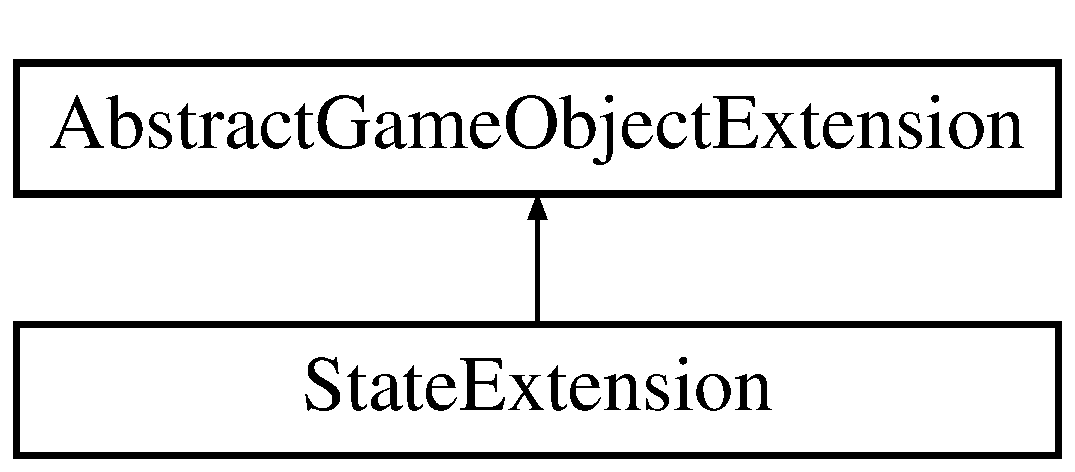
\includegraphics[height=2.000000cm]{class_state_extension}
\end{center}
\end{figure}
\subsection*{Public Member Functions}
\begin{DoxyCompactItemize}
\item 
\mbox{\Hypertarget{class_state_extension_a5560c8d941ebb9ebe875ba59e04613b2}\label{class_state_extension_a5560c8d941ebb9ebe875ba59e04613b2}} 
void {\bfseries change\+State} ()
\end{DoxyCompactItemize}
\subsection*{Static Public Member Functions}
\begin{DoxyCompactItemize}
\item 
\mbox{\Hypertarget{class_state_extension_ae64d01bb34023a2850b7db8f3e47a265}\label{class_state_extension_ae64d01bb34023a2850b7db8f3e47a265}} 
static \mbox{\hyperlink{class_abstract_game_object_extension}{Abstract\+Game\+Object\+Extension}} $\ast$\+\_\+\+\_\+stdcall {\bfseries create} ()
\end{DoxyCompactItemize}
\subsection*{Additional Inherited Members}


The documentation for this class was generated from the following files\+:\begin{DoxyCompactItemize}
\item 
State\+Extension.\+h\item 
State\+Extension.\+cpp\end{DoxyCompactItemize}

\hypertarget{class_switch_extension}{}\section{Switch\+Extension Class Reference}
\label{class_switch_extension}\index{Switch\+Extension@{Switch\+Extension}}
Inheritance diagram for Switch\+Extension\+:\begin{figure}[H]
\begin{center}
\leavevmode
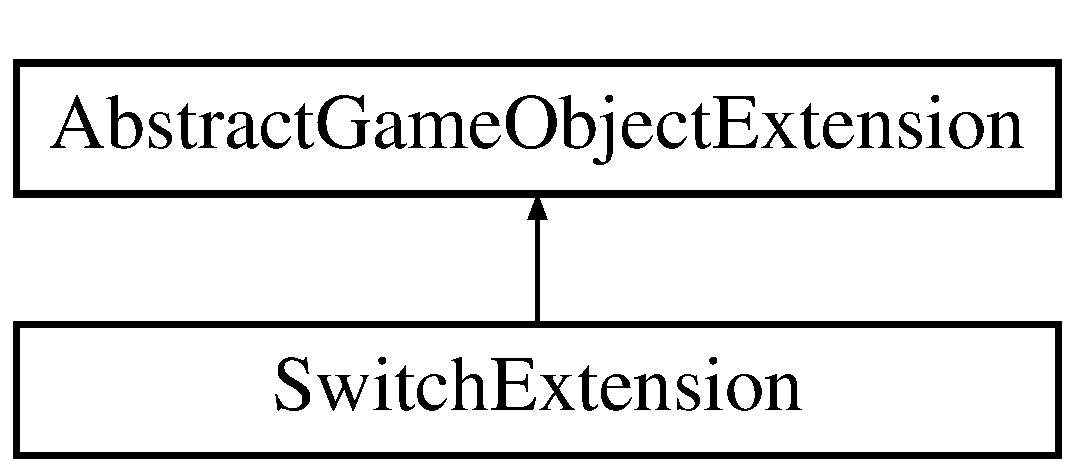
\includegraphics[height=2.000000cm]{class_switch_extension}
\end{center}
\end{figure}
\subsection*{Static Public Member Functions}
\begin{DoxyCompactItemize}
\item 
\mbox{\Hypertarget{class_switch_extension_a501414effe086fa4ceb039939717dd24}\label{class_switch_extension_a501414effe086fa4ceb039939717dd24}} 
static \mbox{\hyperlink{class_abstract_game_object_extension}{Abstract\+Game\+Object\+Extension}} $\ast$\+\_\+\+\_\+stdcall {\bfseries create} ()
\end{DoxyCompactItemize}
\subsection*{Additional Inherited Members}


The documentation for this class was generated from the following file\+:\begin{DoxyCompactItemize}
\item 
Switch\+Extension.\+h\end{DoxyCompactItemize}

\hypertarget{class_text_ui_element}{}\section{Text\+Ui\+Element Class Reference}
\label{class_text_ui_element}\index{Text\+Ui\+Element@{Text\+Ui\+Element}}
Inheritance diagram for Text\+Ui\+Element\+:\begin{figure}[H]
\begin{center}
\leavevmode
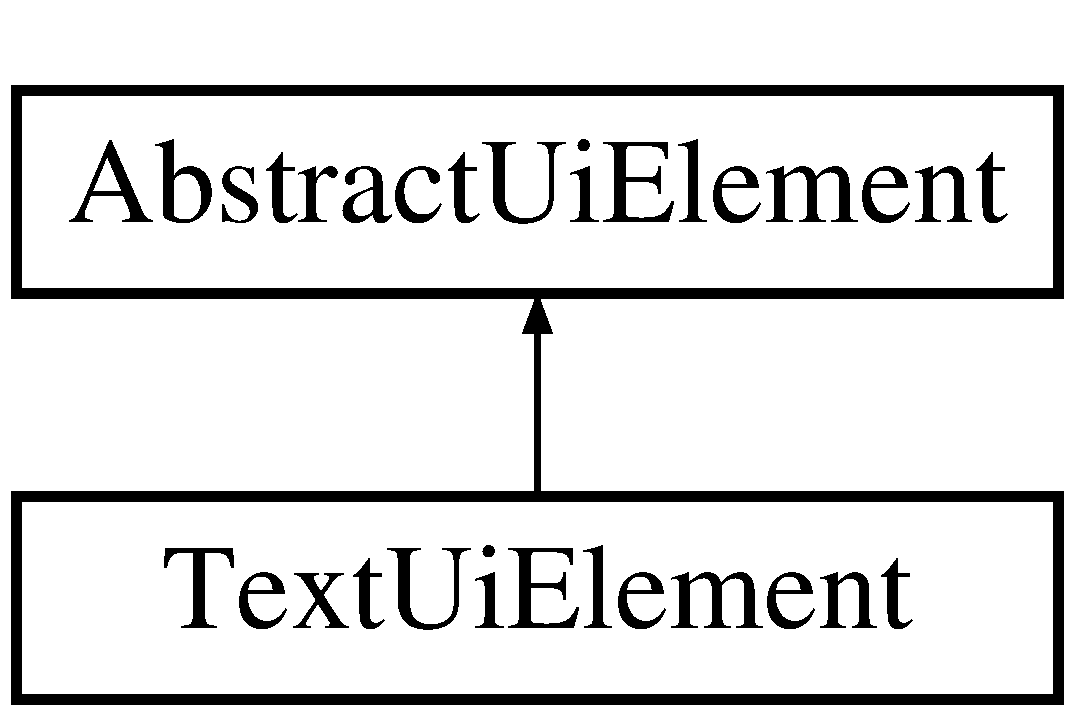
\includegraphics[height=2.000000cm]{class_text_ui_element}
\end{center}
\end{figure}
\subsection*{Public Member Functions}
\begin{DoxyCompactItemize}
\item 
\mbox{\Hypertarget{class_text_ui_element_aa973b38864461eec5942975ad901f0d2}\label{class_text_ui_element_aa973b38864461eec5942975ad901f0d2}} 
{\bfseries Text\+Ui\+Element} (std\+::string txt, std\+::string font\+Key, int font\+Size, \mbox{\hyperlink{struct_rect}{Rect}} rect, \mbox{\hyperlink{struct_color}{Color}} fg\+Color, \mbox{\hyperlink{struct_color}{Color}} bg\+Color, bool center)
\item 
void \mbox{\hyperlink{class_text_ui_element_afe15a4085bc4b7c2cf8668cb6d7fd45d}{pre\+Render}} (\mbox{\hyperlink{class_window}{Window}} $\ast$window)
\item 
void \mbox{\hyperlink{class_text_ui_element_a636883070224511baea505f4ad4655d9}{render}} (\mbox{\hyperlink{class_window}{Window}} $\ast$window)
\begin{DoxyCompactList}\small\item\em Render the element on the screen. \end{DoxyCompactList}\item 
void \mbox{\hyperlink{class_text_ui_element_a984d8bcd627f43c1bd858a707df2c042}{on\+Click}} ()
\begin{DoxyCompactList}\small\item\em The function executed when the element is clicked on. \end{DoxyCompactList}\item 
bool \mbox{\hyperlink{class_text_ui_element_aaf04a9d0a67e77e2ba2a306e1ec7aeed}{is\+In\+Bound}} (int mouseX, int mouseY)
\begin{DoxyCompactList}\small\item\em Checks if the mouse is within the bounds of the element. \end{DoxyCompactList}\end{DoxyCompactItemize}
\subsection*{Additional Inherited Members}


\subsection{Member Function Documentation}
\mbox{\Hypertarget{class_text_ui_element_aaf04a9d0a67e77e2ba2a306e1ec7aeed}\label{class_text_ui_element_aaf04a9d0a67e77e2ba2a306e1ec7aeed}} 
\index{Text\+Ui\+Element@{Text\+Ui\+Element}!is\+In\+Bound@{is\+In\+Bound}}
\index{is\+In\+Bound@{is\+In\+Bound}!Text\+Ui\+Element@{Text\+Ui\+Element}}
\subsubsection{\texorpdfstring{is\+In\+Bound()}{isInBound()}}
{\footnotesize\ttfamily bool Text\+Ui\+Element\+::is\+In\+Bound (\begin{DoxyParamCaption}\item[{int}]{mouseX,  }\item[{int}]{mouseY }\end{DoxyParamCaption})\hspace{0.3cm}{\ttfamily [virtual]}}



Checks if the mouse is within the bounds of the element. 


\begin{DoxyParams}{Parameters}
{\em mouseX} & X coordinate of the mouse\\
\hline
{\em mouseY} & Y coordinate of the mouse\\
\hline
\end{DoxyParams}
\begin{DoxyReturn}{Returns}

\end{DoxyReturn}


Implements \mbox{\hyperlink{class_abstract_ui_element_ad2c415461cd7e8c1ee50b1105eb84685}{Abstract\+Ui\+Element}}.

\mbox{\Hypertarget{class_text_ui_element_a984d8bcd627f43c1bd858a707df2c042}\label{class_text_ui_element_a984d8bcd627f43c1bd858a707df2c042}} 
\index{Text\+Ui\+Element@{Text\+Ui\+Element}!on\+Click@{on\+Click}}
\index{on\+Click@{on\+Click}!Text\+Ui\+Element@{Text\+Ui\+Element}}
\subsubsection{\texorpdfstring{on\+Click()}{onClick()}}
{\footnotesize\ttfamily void Text\+Ui\+Element\+::on\+Click (\begin{DoxyParamCaption}{ }\end{DoxyParamCaption})\hspace{0.3cm}{\ttfamily [virtual]}}



The function executed when the element is clicked on. 



Implements \mbox{\hyperlink{class_abstract_ui_element_a42296c15c9e70b6ac7fda0b1862612af}{Abstract\+Ui\+Element}}.

\mbox{\Hypertarget{class_text_ui_element_afe15a4085bc4b7c2cf8668cb6d7fd45d}\label{class_text_ui_element_afe15a4085bc4b7c2cf8668cb6d7fd45d}} 
\index{Text\+Ui\+Element@{Text\+Ui\+Element}!pre\+Render@{pre\+Render}}
\index{pre\+Render@{pre\+Render}!Text\+Ui\+Element@{Text\+Ui\+Element}}
\subsubsection{\texorpdfstring{pre\+Render()}{preRender()}}
{\footnotesize\ttfamily void Text\+Ui\+Element\+::pre\+Render (\begin{DoxyParamCaption}\item[{\mbox{\hyperlink{class_window}{Window}} $\ast$}]{window }\end{DoxyParamCaption})\hspace{0.3cm}{\ttfamily [virtual]}}

This is called one time before going into the render loop. 


\begin{DoxyParams}{Parameters}
{\em renderer} & The renderer\\
\hline
\end{DoxyParams}


Implements \mbox{\hyperlink{class_abstract_ui_element_a859f627ab385e9d3bf6ce8db40607cdb}{Abstract\+Ui\+Element}}.

\mbox{\Hypertarget{class_text_ui_element_a636883070224511baea505f4ad4655d9}\label{class_text_ui_element_a636883070224511baea505f4ad4655d9}} 
\index{Text\+Ui\+Element@{Text\+Ui\+Element}!render@{render}}
\index{render@{render}!Text\+Ui\+Element@{Text\+Ui\+Element}}
\subsubsection{\texorpdfstring{render()}{render()}}
{\footnotesize\ttfamily void Text\+Ui\+Element\+::render (\begin{DoxyParamCaption}\item[{\mbox{\hyperlink{class_window}{Window}} $\ast$}]{window }\end{DoxyParamCaption})\hspace{0.3cm}{\ttfamily [virtual]}}



Render the element on the screen. 


\begin{DoxyParams}{Parameters}
{\em renderer} & The renderer\\
\hline
\end{DoxyParams}


Implements \mbox{\hyperlink{class_abstract_ui_element_aea66ce333323cf2d5e12d4de9515de7b}{Abstract\+Ui\+Element}}.



The documentation for this class was generated from the following files\+:\begin{DoxyCompactItemize}
\item 
Text\+Ui\+Element.\+h\item 
Text\+Ui\+Element.\+cpp\end{DoxyCompactItemize}

\hypertarget{struct_vec2}{}\section{Vec2 Struct Reference}
\label{struct_vec2}\index{Vec2@{Vec2}}


Helper class for complex operations \& calculations.  




{\ttfamily \#include $<$I\+E\+Math.\+h$>$}

\subsection*{Public Member Functions}
\begin{DoxyCompactItemize}
\item 
\mbox{\Hypertarget{struct_vec2_aa8f28d71ea06633d83c6763122706e4c}\label{struct_vec2_aa8f28d71ea06633d83c6763122706e4c}} 
{\bfseries Vec2} (real x\+\_\+, real y\+\_\+)
\item 
\mbox{\Hypertarget{struct_vec2_acc6bbf6848ff83d15304700d30ea0777}\label{struct_vec2_acc6bbf6848ff83d15304700d30ea0777}} 
void {\bfseries Set} (real x\+\_\+, real y\+\_\+)
\item 
\mbox{\Hypertarget{struct_vec2_abdef2ee4f2eb705a87fe65df3451abdd}\label{struct_vec2_abdef2ee4f2eb705a87fe65df3451abdd}} 
\mbox{\hyperlink{struct_vec2}{Vec2}} {\bfseries operator-\/} (void) const
\item 
\mbox{\Hypertarget{struct_vec2_a8b9af5c711b30c06184af69a3e90884a}\label{struct_vec2_a8b9af5c711b30c06184af69a3e90884a}} 
\mbox{\hyperlink{struct_vec2}{Vec2}} {\bfseries operator$\ast$} (real s) const
\item 
\mbox{\Hypertarget{struct_vec2_aa188e924fa13e126f5078f92297bcc70}\label{struct_vec2_aa188e924fa13e126f5078f92297bcc70}} 
\mbox{\hyperlink{struct_vec2}{Vec2}} {\bfseries operator/} (real s) const
\item 
\mbox{\Hypertarget{struct_vec2_a689c054f9e6c48c5c6d1801e63607164}\label{struct_vec2_a689c054f9e6c48c5c6d1801e63607164}} 
void {\bfseries operator$\ast$=} (real s)
\item 
\mbox{\Hypertarget{struct_vec2_acc8d06b96e3f84cd0cb11e5a17fd046b}\label{struct_vec2_acc8d06b96e3f84cd0cb11e5a17fd046b}} 
\mbox{\hyperlink{struct_vec2}{Vec2}} {\bfseries operator+} (const \mbox{\hyperlink{struct_vec2}{Vec2}} \&rhs) const
\item 
\mbox{\Hypertarget{struct_vec2_add2fd6c94aebeac420f76e21ea02fbd8}\label{struct_vec2_add2fd6c94aebeac420f76e21ea02fbd8}} 
\mbox{\hyperlink{struct_vec2}{Vec2}} {\bfseries operator+} (real s) const
\item 
\mbox{\Hypertarget{struct_vec2_a58f7a9fd50f38f089528cb12af4dd13f}\label{struct_vec2_a58f7a9fd50f38f089528cb12af4dd13f}} 
void {\bfseries operator+=} (const \mbox{\hyperlink{struct_vec2}{Vec2}} \&rhs)
\item 
\mbox{\Hypertarget{struct_vec2_a6c757ff81021ae3ffabf06a6afcdb6bd}\label{struct_vec2_a6c757ff81021ae3ffabf06a6afcdb6bd}} 
\mbox{\hyperlink{struct_vec2}{Vec2}} {\bfseries operator-\/} (const \mbox{\hyperlink{struct_vec2}{Vec2}} \&rhs) const
\item 
\mbox{\Hypertarget{struct_vec2_afb078fac709c7bd64b6c92567a310563}\label{struct_vec2_afb078fac709c7bd64b6c92567a310563}} 
void {\bfseries operator-\/=} (const \mbox{\hyperlink{struct_vec2}{Vec2}} \&rhs)
\item 
\mbox{\Hypertarget{struct_vec2_adb82107cd6ae9725ca606ad64ff1ce36}\label{struct_vec2_adb82107cd6ae9725ca606ad64ff1ce36}} 
real {\bfseries Len\+Sqr} (void) const
\item 
\mbox{\Hypertarget{struct_vec2_ab268b54ca012575edd021412bfdbaf91}\label{struct_vec2_ab268b54ca012575edd021412bfdbaf91}} 
real {\bfseries Len} (void) const
\item 
\mbox{\Hypertarget{struct_vec2_a36c8e58b7451526e4280deef8caf904e}\label{struct_vec2_a36c8e58b7451526e4280deef8caf904e}} 
void {\bfseries Rotate} (real radians)
\item 
\mbox{\Hypertarget{struct_vec2_ab37a161e393133ba7083d3f9386c0173}\label{struct_vec2_ab37a161e393133ba7083d3f9386c0173}} 
void {\bfseries Normalize} (void)
\end{DoxyCompactItemize}
\subsection*{Public Attributes}
\begin{DoxyCompactItemize}
\item 
\mbox{\Hypertarget{struct_vec2_a82bb422b66a9d3d85f8e85c5ad4cc477}\label{struct_vec2_a82bb422b66a9d3d85f8e85c5ad4cc477}} 
\begin{tabbing}
xx\=xx\=xx\=xx\=xx\=xx\=xx\=xx\=xx\=\kill
union \{\\
\>real {\bfseries m} \mbox{[}1\mbox{]}\mbox{[}1\mbox{]}\\
\>real {\bfseries v} \mbox{[}2\mbox{]}\\
\mbox{\Hypertarget{union_vec2_1_1_0D0_a457fc8733fab6c5d599114de82663036}\label{union_vec2_1_1_0D0_a457fc8733fab6c5d599114de82663036}} 
\>struct \{\\
\>\>real {\bfseries x}\\
\>\>real {\bfseries y}\\
\>\} \\
\}; \\

\end{tabbing}\end{DoxyCompactItemize}


\subsection{Detailed Description}
Helper class for complex operations \& calculations. 



The documentation for this struct was generated from the following file\+:\begin{DoxyCompactItemize}
\item 
I\+E\+Math.\+h\end{DoxyCompactItemize}

\hypertarget{class_vision_extension}{}\section{Vision\+Extension Class Reference}
\label{class_vision_extension}\index{Vision\+Extension@{Vision\+Extension}}
Inheritance diagram for Vision\+Extension\+:\begin{figure}[H]
\begin{center}
\leavevmode
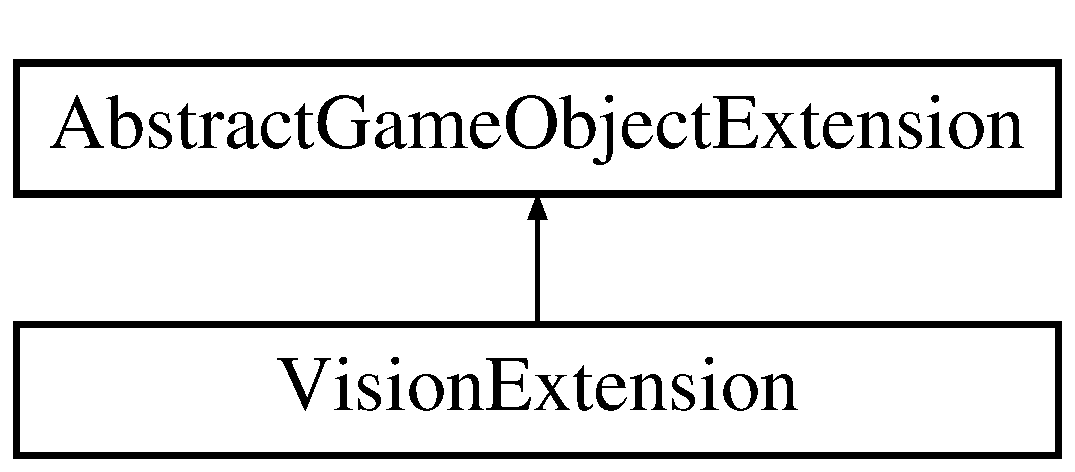
\includegraphics[height=2.000000cm]{class_vision_extension}
\end{center}
\end{figure}
\subsection*{Static Public Member Functions}
\begin{DoxyCompactItemize}
\item 
\mbox{\Hypertarget{class_vision_extension_a56320099331767b9f62a3ccbac4aba06}\label{class_vision_extension_a56320099331767b9f62a3ccbac4aba06}} 
static \mbox{\hyperlink{class_abstract_game_object_extension}{Abstract\+Game\+Object\+Extension}} $\ast$\+\_\+\+\_\+stdcall {\bfseries create} ()
\end{DoxyCompactItemize}
\subsection*{Additional Inherited Members}


The documentation for this class was generated from the following file\+:\begin{DoxyCompactItemize}
\item 
Vision\+Extension.\+h\end{DoxyCompactItemize}

\hypertarget{class_window}{}\section{Window Class Reference}
\label{class_window}\index{Window@{Window}}
\subsection*{Public Member Functions}
\begin{DoxyCompactItemize}
\item 
\mbox{\Hypertarget{class_window_a315084d17424d10fe4a77c581084b65a}\label{class_window_a315084d17424d10fe4a77c581084b65a}} 
{\bfseries Window} (const char $\ast$title, int width, int height)
\item 
\mbox{\Hypertarget{class_window_a27f9206967e022a50e0471fe43fcf73c}\label{class_window_a27f9206967e022a50e0471fe43fcf73c}} 
S\+D\+L\+\_\+\+Window $\ast$ {\bfseries get\+Window} () const
\item 
\mbox{\Hypertarget{class_window_aee31a875d654a8c8f7d796d072657791}\label{class_window_aee31a875d654a8c8f7d796d072657791}} 
int {\bfseries get\+Width} () const
\item 
\mbox{\Hypertarget{class_window_a60757b2b0dbcec9889e3a09f5655adbe}\label{class_window_a60757b2b0dbcec9889e3a09f5655adbe}} 
int {\bfseries get\+Height} () const
\item 
\mbox{\Hypertarget{class_window_a38bc43bdd1a97e5de7f346ba4c3957ef}\label{class_window_a38bc43bdd1a97e5de7f346ba4c3957ef}} 
void {\bfseries clear} ()
\item 
\mbox{\Hypertarget{class_window_afadfafa5a0b9472554759004aafb327e}\label{class_window_afadfafa5a0b9472554759004aafb327e}} 
void {\bfseries display} ()
\item 
\mbox{\Hypertarget{class_window_a876e244f06eb219cb8c6ce1bb70b2631}\label{class_window_a876e244f06eb219cb8c6ce1bb70b2631}} 
void {\bfseries register\+Texture} (std\+::string texture\+Key, std\+::string texture\+Path)
\item 
\mbox{\Hypertarget{class_window_ae6774de63023e68fd6bb101667bab9c1}\label{class_window_ae6774de63023e68fd6bb101667bab9c1}} 
void {\bfseries register\+Font} (std\+::string font\+Key, std\+::string font\+Path)
\item 
\mbox{\Hypertarget{class_window_a64492bfdd5d0a57809a2a654588c280f}\label{class_window_a64492bfdd5d0a57809a2a654588c280f}} 
S\+D\+L\+\_\+\+Texture $\ast$ {\bfseries get\+Texture} (std\+::string file\+Path) const
\item 
\mbox{\Hypertarget{class_window_a13b85acfb08ad3ab526bbe71158c7dcc}\label{class_window_a13b85acfb08ad3ab526bbe71158c7dcc}} 
T\+T\+F\+\_\+\+Font $\ast$ {\bfseries get\+Font} (std\+::string font\+Key, int font\+Size)
\item 
\mbox{\Hypertarget{class_window_a94011a77192e38baa21bb3e86ffabf8c}\label{class_window_a94011a77192e38baa21bb3e86ffabf8c}} 
void {\bfseries render\+Rectangle} (\mbox{\hyperlink{struct_rect}{Rect}} rect, \mbox{\hyperlink{struct_color}{Color}} color)
\item 
\mbox{\Hypertarget{class_window_ac523b07058eac58d3c4dd27d52aba51d}\label{class_window_ac523b07058eac58d3c4dd27d52aba51d}} 
void {\bfseries render\+Texture} (std\+::string texture\+Key, \mbox{\hyperlink{struct_rect}{Rect}} rect)
\item 
\mbox{\Hypertarget{class_window_ae9a460a8d85af7da21fabb4ee2d24169}\label{class_window_ae9a460a8d85af7da21fabb4ee2d24169}} 
void {\bfseries render\+Text} (std\+::string text, T\+T\+F\+\_\+\+Font $\ast$font, \mbox{\hyperlink{struct_rect}{Rect}} rect, \mbox{\hyperlink{struct_color}{Color}} foreground\+Color, \mbox{\hyperlink{struct_color}{Color}} background\+Color, bool center)
\end{DoxyCompactItemize}


The documentation for this class was generated from the following files\+:\begin{DoxyCompactItemize}
\item 
Window.\+h\item 
Window.\+cpp\end{DoxyCompactItemize}

%--- End generated contents ---

% Index
\backmatter
\newpage
\phantomsection
\clearemptydoublepage
\addcontentsline{toc}{chapter}{Index}
\printindex

\end{document}
